%%%%%%% Document settings %%%%%%%%%%
\documentclass{DESSThesis}


%%%%%%%%%%% Additional Packages %%%%%%%%%%%%%%%%%%%%%%%%%%%
\usepackage{{booktabs}}
\usepackage{subcaption}
\usepackage{algorithm}
\usepackage{algorithmic}
\usepackage{fancyhdr}
\usepackage{microtype}
\usepackage{tikz}
\usepackage{pgfgantt}
\usepackage{lscape}
\pgfplotsset{compat=1.18}
\usepackage{graphicx}
\usepackage[table,xcdraw]{xcolor}
\usepackage{scrlayer-scrpage}
\usepackage{scrhack}
\usepackage{float}
\usepackage{caption}


\usepackage{amsmath,amssymb}
\usepackage{url}
\usepackage{textcomp}
\newcommand{\code}[1]{\texttt{#1}}
\DeclareMathOperator*{\argmax}{arg\,max}


%%%%%%%%%%%%%%%%%%%%%% Hyphenations %%%%%%%%%%%%%%
\hyphenation{trac-ta-ble}


%%%%%%%%%%%%%%%%%%%%%%%%%%%%%%%%%%%%%%%%%%%%%%%%%%
\overfullrule=2cm
\bibliography{final_thesis}
\begin{document}
\let\cleardoublepage\clearpage

%%%%%%%%%%%%%%%%%%%%% Frontpage %%%%%%%%%%%%%%%%%%%%%%%%%%%%%%%
\def \TypeofThesis{Master Thesis}
\def \TitleofThesis{Personality Assessment of Language Models using Task Arithmetic and PEFT}
\def \AuthorofThesis{Prayag Bhattarai\\MSc. Business Informatics\\1825720}
\def \FirstSupervisor{Prof. Dr. Markus Strohmaier}
\def \Advisor{Georg Ahnert}
%%%%%%%%%%%%%%%%%%%%%%%%%%%%%%%%%%%%%%%%%
% Academic Title Page
% LaTeX Template
% Version 2.0 (17/7/17)
%
% This template was downloaded from:
% http://www.LaTeXTemplates.com
%
% Original author:
% WikiBooks (LaTeX - Title Creation) with modifications by:
% Vel (vel@latextemplates.com)
% Lorena Reintgen
%
% License:
% CC BY-NC-SA 3.0 (http://creativecommons.org/licenses/by-nc-sa/3.0/)
% 
%
%%%%%%%%%%%%%%%%%%%%%%%%%%%%%%%%%%%%%%%%%

%----------------------------------------------------------------------------------------
% TITLE PAGE
%----------------------------------------------------------------------------------------

\begin{titlepage} % Suppresses displaying the page number on the title page and the subsequent page counts as page 1
\newcommand{\HRule}{\rule{\linewidth}{0.5mm}} % Defines a new command for horizontal lines, change thickness here
\center % Centre everything on the page
%\renewcommand{\baselinestretch}{1.2} %vertical spacing between lines
%------------------------------------------------
%  Headings
%------------------------------------------------
\textsc{\LARGE \TypeofThesis}\\[1.5cm] % Main heading such as the name of your university/college
%------------------------------------------------
%  Title
%------------------------------------------------
\HRule\\[0.4cm]
{\huge\bfseries \TitleofThesis}\\[0.4cm] % Title of your document
\HRule\\[1.5cm]
%------------------------------------------------
%  Author(s)
%------------------------------------------------
    \vfill
    \textit{\large submitted by}\\[0.5cm] % Major heading
\textsc{\Large \AuthorofThesis}\\[0.5cm] % Minor heading
    \vfill

{\large\textit{Submitted to the}}\\
\Large Chair for Data Science in the Economic and Social Sciences \\
    {\large\textit{within the}}\\
    Faculty of Business Administration \\
    at University of Mannheim 
    
    %------------------------------------------------
%  Date
%------------------------------------------------
\vfill\vfill\vfill % Position the date 3/4 down the remaining page
{\large\today} % Date, change the \today to a set date if you want to be precise

\vfill\vfill\vfill
{ \large \center 
\textit{Advisor:}\\
\Advisor
}
\vfill\vfill\vfill
{ \large \center 
\textit{Supervisor:}\\
\FirstSupervisor
}
% \vfill
%     \begin{minipage}{0.48\textwidth}
% \begin{flushleft}
% \large
% \textit{First Supervisor}\\
% \FirstSupervisor
% \end{flushleft}
% \end{minipage}
% ~
% \begin{minipage}{0.48\textwidth}
% \begin{flushright}
% \large
% % \textit{Second Supervisor}\\
% % \SecondSupervisor
% \end{flushright}
% \end{minipage}

%------------------------------------------------
%  Logo
%------------------------------------------------
%\vfill\vfill
%\includegraphics[width=0.2\textwidth]{placeholder.jpg}\\[1cm] % Include a department/university logo - this will require the graphicx package
 
%----------------------------------------------------------------------------------------
\vfill % Push the date up 1/4 of the remaining page
\end{titlepage}

%\vfill
% \cleardoublepage

\tableofcontents


%%%%%%%%%%%%%%%%%%%%% Abstract & Abbreviations %%%%%%%%%%%%%%%%%%%%%%%%%%%%%
\chapter*{List of Abbreviations}
\addcontentsline{toc}{chapter}{List of Abbreviations}
\begin{description}
\item[NLP] Natural Language Processing
\item[(L)LM] (Large) Language Model
\item[PEFT] Parameter-Efficient Fine-Tuning
\item[LoRA] Low-Rank Adaptation
  \item[OCEAN] Openness, Conscientiousness, Extraversion, Agreeableness, Neuroticism
\item[MBTI] Myers-Briggs Type Indicator
\item[SoTA] State-of-the-art
\end{description}

\newpage
\thispagestyle{plain}
\begin{abstract}
Given the documented instabilities of current evaluation approaches, the proliferation of Large Language Models (LLMs) with human-like personalities and emotional expressions calls for rigorous methodologies for their assessment and control. The usefulness of Parameter-Efficient Fine-Tuning (PEFT), in particular Low-Rank Adaptation (LoRA), and Task Arithmetic for observing, adjusting, and assessing these emergent psychological constructs is systematically investigated in this thesis. Experiments using the GPT-2 architecture included fine-tuning on selected data splits from the TweetEval-Emotion (PANAS-X affective dimensions) and PANDORA (Big Five OCEAN personality) datasets. With an emphasis on the effects of different adapter scaling factors, LoRA was used for effective adaptation. By building LoRA adapters that were trained on particular characteristics or emotions and using base models that were adjusted based on various psychological dimensions, task arithmetic was investigated. The BFI-10, IPIP-120, and PANAS-X psychometric inventories were used for evaluation. They were given using a new likelihood-based scoring pipeline that was made to account for some prompt sensitivities.
\\
The following key findings show that: (1) Targeted fine-tuning on trait-specific data directionally shifts perceived personality and emotion scores in LLMs, although emotional dimensions show subtle co-amplification effects. (2) The intensity of expressed traits can be modulated through a non-linear yet powerful mechanism provided by LoRA adapter scaling, which reveals intricate response curves with saturation and rebound effects at extreme scaling values. (3) Task Arithmetic operations can successfully modify the behavioral profiles of LLMs in a way that is consistent with psychological theory by composing learned trait/emotion vectors using LoRA adapters. This allows for the creation of complex psychological states. (4) The custom likelihood-based evaluation pipeline demonstrated consistency across various personality psychometric instruments and relative robustness to slight prompt variations (inclusion/exclusion of explicit response options).
\\
This study offers methodological insights and empirical support for the rigorous evaluation and controlled manipulation of psychological traits in LLMs. It shows how PEFT and Task Arithmetic can be used for fine-grained behavioral control in the domain of simulated personality and emotion, which advances the possibility of creating more predictable, steerable, and morally aware AI systems.
\\
\\
\textbf{Keywords:} LMs | Task Arithmetic | PEFT | Psychometrics
\end{abstract}

\cleardoublepage
\pagenumbering{arabic}


%%%%%%%%%%%%%%%%%%%%% Chapter 1 %%%%%%%%%%%%%%%%%%%%%%
\chapter{Introduction}
\thispagestyle{empty}

\subsection{Background \& Motivation}
\subsubsection{Defining Personality and Emotion in Humans}
Understanding the persistent patterns in people's thoughts, feelings, and behaviors—collectively referred to as personality—has long been a goal of the study of human individuality. Openness, Conscientiousness, Extraversion, Agreeableness, and Neuroticism (OCEAN) are the five dimensions that psychological theories, particularly the Five-Factor Model (FFM), suggest can be used to broadly characterize personality \cite{feng_five-factor_2024,mccrae_reinterpreting_1989,okeefe_introducing_2012}. Although there are other frameworks, such as the Myers-Briggs Type Indicator (MBTI), their scientific validity for rigorous assessment is still up for debate \cite{mccrae_reinterpreting_1989,li_influence_2018}. Emotions, which are typically regarded as more ephemeral affective states, are distinct from these stable characteristics. They include moods and feelings that can change in response to different stimuli \cite{david_watson_panas-x_1994,barsade_ripple_2002}. Both the general aspects of affect (Positive and Negative Affect) and more specialized emotional states like fear or joviality can be measured with tools like the Positive and Negative Affect Schedule-Expanded Form (PANAS-X) \cite{david_watson_panas-x_1994}. Much of human experience and social interaction is defined by the intricate interplay between these stable personality traits and ephemeral emotional states \cite{hochschild_emotion_1979,lerner_emotion_2015}.

\subsubsection{Emergence of Personality and Emotion in LLMs}
Large Language Models (LLMs) that can produce text that is strikingly human-like have been developed as a result of recent developments in artificial intelligence. Their propensity to exhibit behaviors and linguistic patterns that humans interpret as representative of personality or emotional expression is an intriguing emergent property of these models \cite{jiang_evaluating_2023,pan_llms_2023,safdari_personality_2023,chang_modeling_2024}. The enormous amounts of human-generated text data that these models are trained on, along with their underlying architecture and subsequent fine-tuning procedures, are believed to have influenced these perceived qualities, which are not explicitly programmed \cite{frisch_llm_2024,gupta_self-assessment_2024,sorokovikova_llms_2024}. For example, LLMs have been found to produce text that can be categorized as expressing particular emotions or sentiments \cite{liu_emollms_2024,paech_eq-bench_2024} and to complete personality questionnaires in ways that suggest distinct profiles \cite{safdari_personality_2023,caron_identifying_2022}.

\subsubsection{Significance of Studying Personality/Emotion in LLMs}
The finding that LLMs can display emotional expressions and personality-like traits has important ramifications for how they are developed and used. It is essential to comprehend and possibly manage these traits for a number of reasons. First of all, it can result in improved control over digital assistants and conversational agents, enabling more efficient and customized human-computer interaction \cite{zhang_better_2024,mao_editing_2024}. Second, researchers may be able to examine how various personality traits may affect responses or interactions in simulated environments by using LLMs with observable and controllable personas as useful tools for social simulation \cite{song_identifying_2024,mozikov_good_2024}. According to \cite{safdari_personality_2023,chang_modeling_2024,sabour_emobench_2024}, the perceived personality and emotional tone of an LLM can profoundly affect user trust, engagement, and the overall ethical considerations of its use, including the possibility of bias amplification or unintended influence.

\subsubsection{Current Methodologies For LLM Personality/Emotion Assessment}
To evaluate these emergent characteristics in LLMs, researchers have started to modify approaches from human psychology. Standardized human psychometric tools, like the Myers-Briggs Type Indicator (MBTI) or the Big Five Inventory (BFI), are frequently given to LLMs directly by prompting them with questionnaire items \cite{caron_identifying_2022,pan_llms_2023,sorokovikova_llms_2024}. Others concentrate on examining the linguistic characteristics of LLM-generated text using tools such as LIWC to determine personality \cite{jiang_personallm_2024,hilliard_eliciting_2024} or create new benchmarks especially made to assess emotional intelligence or understanding in LLMs \cite{paech_eq-bench_2024,wang_emotional_2023,sabour_emobench_2024}. These techniques seek to measure how closely LLM results match human ideas of emotion and personality.

\subsubsection{PEFT \& Task Arithmetic}
Significant progress has been made in techniques for effectively adapting these large models in tandem with the investigation of LLM characteristics. The prohibitive computational costs of fully fine-tuning multi-billion parameter models have led to the development of Parameter-Efficient Fine-Tuning (PEFT) techniques \cite{houlsby_parameter-efficient_2019,lialin_scaling_2023}. Among these, Low-Rank Adaptation (LoRA) has become well-known for its ability to update a small portion of the model parameters by adding trainable low-rank matrices to pre-existing layers, while still performing on many tasks as well as full fine-tuning \cite{hu_lora_2021,mao_survey_2025}.
\\
At the same time, model editing methods such as Task Arithmetic provide ways to modify the behavior of the model by executing arithmetic operations on its "task vectors," which are the modifications brought about by fine-tuning on particular tasks \cite{ilharco_editing_2023,chronopoulou_language_2023}. These methods present opportunities for more precise control over model behaviors, such as those pertaining to perceived personality and emotion, in addition to effective specialization.

\subsubsection{Underlying Motivation}
The main question of this thesis is motivated by the emergence of personality/emotion-like behaviors in LLMs, the creation of techniques to evaluate these behaviors, and the introduction of effective, potent adaptation strategies like Task Arithmetic and LoRA. Although current research has started to define LLM "personalities" and "emotions," more thorough research is required to determine how these characteristics can be robustly expressed, controlled, and measured with accuracy. This thesis is specifically driven by the possibility of using fine-tuning on personality and emotion-specific data, along with the compositional power of Task Arithmetic and the nuanced control provided by LoRA scaling, to better understand how these important anthropomorphic traits are assessed and altered in LLMs.

\subsection{Problem Statement \& Research Gap}

\subsubsection{Limitations of Current LLM Personality/Emotion Assessment}
The validity and reliability of current approaches are seriously questioned, despite the growing interest in evaluating personality and emotion in LLMs. One major issue is the direct use of personality tests based on human self-assessment, which has been demonstrated to produce inconsistent and unstable results \cite{gupta_self-assessment_2024,shu_you_2024,suhr_challenging_2023,tommaso_llms_2024}. Human responses are generally robust to minor variations in prompt phrasing and the order of multiple-choice options, but LLMs are extremely sensitive to these factors \cite{gupta_self-assessment_2024,shu_you_2024,zheng_lmlpa_2024}. Furthermore, it is possible that the tests are not measuring the same underlying constructs in LLMs as they do in humans because LLMs frequently fail to replicate the stable factor structures (such as the five factors of the Big Five model) seen in human psychometric data \cite{suhr_challenging_2023}. With responses fluctuating over brief time periods, the temporal stability of LLM-exhibited traits is also restricted, raising concerns about whether these models have "enduring characteristics" in the human sense \cite{bodroza_personality_2024,tommaso_llms_2024}. Similarly, dataset biases, the models' dependence on surface-level patterns rather than in-depth knowledge, and the subjectivity involved in defining and measuring emotional responses make it difficult to assess emotional intelligence in LLMs \cite{sabour_emobench_2024,paech_eq-bench_2024}.

\subsubsection{Gaps in Understanding Controllability and Robustness}
Although methods like prompt engineering and fine-tuning have shown promise in influencing LLMs' perceived personalities and emotional expression \cite{caron_identifying_2022,jiang_evaluating_2023,mao_editing_2024,chang_modeling_2024}, there is still a great deal to learn about how these characteristics can be reliably and methodically managed and assessed. Task Arithmetic's potential for creating or altering certain personality or emotional traits, as well as the effectiveness of more recent, more effective techniques like PEFT (more especially LoRA) for inducing and scaling these traits, have not been thoroughly investigated in a single experimental framework. The relationship between LoRA scaling parameters and the intensity of expressed traits is an area that needs more thorough research, as previous studies on PEFT for personality or emotion frequently concentrate on particular models or small sets of traits. Furthermore, a crucial but little-studied factor is the robustness of any induced changes—their consistency across various assessment tools and their resistance to slight prompt variations.

\subsubsection{Need for Systematic Investigation}
Given the current situation, a thorough examination of the evaluation and control of personality and emotion in LLMs using sophisticated, effective methods is urgently needed. In particular, little research has been done that combines the compositional capabilities of Task Arithmetic and the precise control provided by LoRA scaling with fine-tuning on carefully selected personality/emotion-specific data splits. A major research gap exists in understanding how these approaches interact and affect the quantifiable personality and emotional expression of LLMs, as well as critically evaluating the robustness and generalizability of these effects. By offering a systematic empirical examination of these interrelated elements, this thesis seeks to close this gap.

\subsection{Research Objectives \& Questions}

\subsubsection{Primary Research Goal}
Measuring, modifying, and analyzing perceived personality and emotion-like traits in large language models is the main objective of this study. This entails examining the effects of focused fine-tuning tactics, the scalability of trait expression through the use of Parameter-Efficient Fine-Tuning (PEFT) methods such as LoRA, and the possibility of using Task Arithmetic to alter these behavioral profiles.

\subsubsection{Specific Objectives}
To achieve the primary goal, this thesis pursues the following specific objectives:
\begin{enumerate}
\item to find out if adjusting LLMs on text data that represents the extremes of particular personality (Big Five) and emotion (PANAS-X) dimensions causes their measured trait scores to change in a way that is consistent with the changes.
\item In order to ascertain whether trait expression can be systematically turned up or down, it is necessary to investigate how different LoRA scaling factors affect the intensity of expressed personality and emotion traits.
\item to investigate how task arithmetic operations, like adding or subtracting task vectors from models that have been adjusted based on particular personality/emotion data, can be used to alter the overall emotional and personality profile of an LLM.
\item To evaluate consistency across various psychometric instruments (PANAS-X for emotion; BFI-10 and IPIP-120 for personality) and to analyze sensitivity to slight variations in prompting techniques during evaluation in order to determine the robustness of any observed changes in personality and emotion.
\end{enumerate}

\subsubsection{Research Questions}
Based on these objectives, this thesis seeks to answer the following research questions:
\begin{itemize}
\item \textbf{RQ1}: How do the scores on corresponding psychometric inventories change when an LLM is fine-tuned on data splits that represent high or low expressions of particular Big Five personality traits and PANAS-X affective dimensions?
\item \textbf{RQ2}: Does the measured intensity of the targeted personality or emotion traits in the LLM's responses have a consistent relationship with the LoRA scaling factor used during fine-tuning?
\textbf{RQ3}: If so, how can arithmetic operations on task vectors from LLMs tuned on different personality or emotion profiles effectively change how these traits are expressed in a base model?
\textbf{RQ4}: How sensitive are these tests to changes in the prompting protocol used for evaluation, and how consistent are the personality and emotion profiles seen following fine-tuning and LoRA scaling when evaluated using various psychometric tools?
\end{itemize}

\subsection{Hypotheses}

\subsubsection{Hypothesis 1 (Fine-tuning Effect)}
Using text data from people who have high levels of a particular personality trait (like extraversion) or emotional state to fine-tune a language model is thought to increase the likelihood that the model will display linguistic patterns and produce responses that are consistent with an amplified expression of that same trait when it is later evaluated. Targeted fine-tuning should change the behavioral tendencies of LLMs, as they are known to imitate patterns in their training data \cite{jiang_evaluating_2023,pan_llms_2023,safdari_personality_2023}.
\begin{itemize}
\item \textbf{H1}: Using text from individuals who score highly on Trait X to fine-tune a model increases the likelihood that the model will display or amplify that trait in its responses.
\end{itemize}

\subsubsection{Hypothesis 2 (LoRA Scaling Effect)}
It is postulated that the scaling factor applied to LoRA adapters can function as a control mechanism for the intensity of trait expression, building on the parameter-efficient nature of LoRA, which enables targeted updates to model behavior. According to psychometric inventories, systematically increasing this scaling factor should result in a correspondingly more pronounced manifestation of the targeted personality or emotion trait in the model's outputs \cite{hu_lora_2021,lialin_scaling_2023,zhao_lora_2024}.
\begin{itemize}
\item \textbf{H2}: Increasing the LoRA scaling factor systematically intensifies the expression of that trait in the model’s responses.
\end{itemize}

\subsubsection{Hypothesis 3 (Task Arithmetic Effect)}
Through arithmetic on model weight differences (task vectors), Task Arithmetic has shown that it is possible to isolate or combine learned capabilities. Therefore, it is hypothesized that using such operations, such as adding the task vector of a model that has been fine-tuned on text from highly extraverted people and subtracting the task vector from a model that has been fine-tuned on text from highly introverted people (or text that expresses negative emotions), will cause the personality profile of a base model to shift toward the traits that the added vectors emphasize, thereby amplifying related behavioral traits \cite{ilharco_editing_2023,chronopoulou_language_2023}.
\begin{itemize}
    \item \textbf{H3}: Arithmetic operations on task vectors (e.g., adding top 5\% and subtracting bottom 5\% or negative emotion vectors) shift the model’s personality profile toward the traits emphasized in the added vectors, amplifying associated behavioral characteristics.
\end{itemize}

\subsection{Assumptions, Scope \& Delimitations}

\subsubsection{Scope of Personality/Emotion Constructs}
The assessment and manipulation of personality traits as outlined by the Five-Factor Model (OCEAN, or openness, conscientiousness, extraversion, agreeableness, and neuroticism) will be the main focus of this study. The Big Five Inventory-10 (BFI-10) and the International Personality Item Pool 120-item version (IPIP-120) will be the main tools used to evaluate personality. The Positive and Negative Affect Schedule - Expanded Form (PANAS-X) will be used in the study to measure both more specific emotional states and broad aspects of positive and negative affect.

\subsubsection{Scope of LLMs}
GPT-2, an autoregressive large language model, will be used for the experiments. Later in the methodology chapter, the reasoning behind the choice of this model is explained.

\subsubsection{Scope of Techniques}
As the main Parameter-Efficient Fine-Tuning (PEFT) technique, the study will focus on Low-Rank Adaptation (LoRA). We will look into specific LoRA configurations, especially the manipulation of its scaling factor. The study will investigate simple arithmetic operations (addition, subtraction) on task vectors obtained from optimized models in order to edit the model.

\subsubsection{Assumptions}
The following assumptions underpin this research:
\begin{enumerate}
\item It is assumed that LLM-generated text can be meaningfully examined for patterns that match human-perceived emotional expressions and personality traits when responding to psychometric questionnaire items or scenarios. It is believed that measuring these "traits" in LLMs using modified tools will yield measurable insights into model behavior, even though their nature differs from human psychological states.
\item It is assumed that there are enough unique linguistic cues linked to the desired traits and affective states in the PANDORA dataset for personality and the TweetEval-Emotion dataset for emotion to allow for efficient LLM fine-tuning.
\item It is believed that the BFI-10, IPIP-120, and PANAS-X evaluation tools, as well as the unique Likert-scale scoring pipeline created for this thesis, are suitable and sensitive enough to measure the desired personality and emotion-like constructs in the textual outputs of LLMs.
\end{enumerate}

\subsubsection{Delimitations}
The research is subject to the following delimitations:
\begin{enumerate}
\item In terms of human psychology, this study makes no claims regarding the existence of true consciousness, subjective emotions, or personality in LLMs. The scope of the study is strictly restricted to discernible patterns in their language output that can be quantified and analyzed using theories of emotion and human personality.
\item The full range of PEFT techniques and all potential variants of Task Arithmetic will not be investigated in this study. To keep things tractable, the emphasis will be on particular, representative LoRA configurations and basic arithmetic operations.
\item English-language LLMs, datasets, and evaluation tools will be used for all experiments and analyses. It's possible that the results don't apply directly to other languages.
\item Robustness checks will concentrate on sensitivity to small changes in the evaluation prompting protocol, the impact of using different data splits for evaluation and fine-tuning, and consistency across questionnaires for the same construct (e.g., BFI-10 vs. IPIP-120 for personality). It is outside the purview of this thesis to thoroughly investigate every possible source of instability or confounding factor.
\item Instead of thoroughly examining downstream behavioral consequences in intricate interactive tasks, the study will mainly concentrate on the direct effects of task arithmetic, LoRA scaling, and fine-tuning on measured traits.
\end{enumerate}



%%%%%%%%%%%%%%%%%%%%% Chapter 2 %%%%%%%%%%%%%%%%%%%%%%
\chapter{Conceptual Foundations}
\thispagestyle{empty}

By examining the psychological concepts of personality and emotion, this chapter establishes the theoretical framework for the thesis. It explores accepted theories, widely used measurement techniques, and the complex interrelationship between these two essential facets of human experience. Prior to analyzing their counterparts or simulations in computational systems such as Large Language Models (LLMs), it is essential to comprehend these human-centric concepts.

\subsection{Personality: Psychological Theories \& Measurement}
\subsubsection{Defining Personality}
In psychological science, personality refers to persistent thought, emotion, and behavior patterns that define a person and set them apart from others. Particularly in adulthood, these patterns show stability over time and relative consistency across various contexts \cite{feng_five-factor_2024,mccrae_reinterpreting_1989}. Modern psychology has attempted to define and measure personality through empirical investigation, often conceptualizing it as a set of traits or non-cognitive skills that influence an individual's interactions with the world \cite{kamarulzaman_confirmatory_2012,cobb-clark_stability_2012}. This is in contrast to early philosophical inquiries that pondered the nature of human individuality.

\subsubsection{The Five-Factor Model (FFM)}
The Five-Factor Model (FFM), also referred to as the Big Five, is the most widely recognized and empirically supported model among different theoretical frameworks for characterizing personality at a broad level of abstraction \cite{feng_five-factor_2024,okeefe_introducing_2012,rammstedt_big_2014}. The acronym OCEAN stands for Openness to Experience (creativity, intellectual curiosity), Conscientiousness (organization, dependability), Extraversion (sociability, assertiveness), Agreeableness (cooperativeness, empathy), and Neuroticism (emotional instability, proneness to negative emotions). This model suggests that the majority of individual differences in personality can be captured by these five fundamental dimensions. According to \cite{feng_five-factor_2024}, the FFM is regarded as an empirical generalization that was developed from consistent patterns in personality traits found in a variety of populations and assessment techniques.

\subsubsection{Lexical Hypothesis and FFM Development}
The lexical hypothesis, which holds that the most significant individual differences in human transactions will eventually be encoded as single terms in some or all of the world's languages, is a major foundation for the development of the FFM \cite{rammstedt_big_2014,feng_five-factor_2024}. Following pioneers like Cattell's reduction of lengthy lists of personality-descriptive adjectives from dictionaries through factor analysis, later researchers like Norman and Goldberg \cite{feng_five-factor_2024} consistently identified five key factors. At least within Western language families, this linguistic basis emphasizes the model's cross-cultural reproducibility and link to everyday language \cite{rammstedt_big_2014}.

\subsubsection{Hierarchical Structure and Facet-Level Assessment}
According to \cite{kajonius_assessing_2019,maples_test_2014}, the FFM is a hierarchical structure in which the five broad domains encompass more specialized, lower-order facet traits. Facet-level analysis offers a more detailed understanding and can provide higher precision for specific applications, such as differentiating clinical diagnoses or job candidates, whereas domain scores offer a broad overview \cite{kajonius_assessing_2019}. These aspects, usually six for each of the five domains, are measured by tools such as the NEO Personality Inventory-Revised (NEO PI-R) and its public-domain equivalents, such as the IPIP-NEO-120 \cite{johnson_measuring_2014,maples_test_2014}.

\subsubsection{Measurement Instruments and Psychometric Properties}
In the FFM, personality traits are primarily assessed through self-report questionnaires in which respondents score how well they are described by different adjectives, phrases, or sentences \cite{feng_five-factor_2024,johnson_measuring_2014}. Examples include the Big Five Inventory (BFI), the NEO PI-R, and tools from the International Personality Item Pool (IPIP), including the shorter BFI-10 and the IPIP-NEO-120 \cite{maples_test_2014,johnson_measuring_2014,rammstedt_big_2014}. These tools were developed and validated with an emphasis on psychometric properties such as construct validity (convergent, discriminant, and factorial validity), temporal stability (test-retest reliability), and internal consistency reliability (e.g., Cronbach's alpha) \cite{johnson_measuring_2014,rammstedt_big_2014,kajonius_assessing_2019}. A key statistical tool for determining whether the empirical structure of questionnaire responses matches the theoretical FFM structure is factor analysis, both exploratory (EFA) and confirmatory (CFA) \cite{kajonius_assessing_2019,kamarulzaman_confirmatory_2012}.

\subsubsection{Stability of Personality Traits}
The significant stability of personality traits, especially the Big Five, is a crucial feature, especially for working-age adults. Although not strictly immutable, longitudinal studies, like those that use the HILDA survey, have demonstrated that the Big Five traits show modest average changes over time, such as four years, and that these changes typically do not vary significantly with age within this demographic \cite{cobb-clark_stability_2012}. Although some research suggests greater malleability during adolescence or in response to significant life events, but the latter's impact on core traits appears limited in working-age adults, this relative stability supports the conceptualization of personality as an enduring characteristic \cite{cobb-clark_stability_2012}.

\subsubsection{Predictive Validity of Personality}
For many important life outcomes, the FFM dimensions have shown predictive validity. For example, conscientiousness and neuroticism are associated with longevity and health; conscientiousness, openness, conscientiousness, and agreeableness influence career choices and success; and conscientiousness, extraversion, and emotional stability (low neuroticism) are associated with job satisfaction \cite{rammstedt_big_2014,kajonius_assessing_2019}. Predicting such results highlights the usefulness of personality testing beyond description \cite{kosinski_private_2013}.

\subsubsection{Alternative Models and Critiques (MBTI)}
There are alternative personality models, such as the Myers-Briggs Type Indicator (MBTI), despite the dominance of the FFM. Based on Jungian theory, the MBTI divides people into two categories: extraversion and introversion, sensing and intuition, etc. However, when compared to the continuous trait distributions found in FFM research, its scientific validity and reliability have been called into question, especially its typological assumptions that lack empirical support \cite{mccrae_reinterpreting_1989,li_influence_2018}. According to studies, MBTI scales primarily assess four of the five FFM dimensions, indicating that it is more appropriate to view it as a trait measure as opposed to a typological one \cite{mccrae_reinterpreting_1989}.

\subsection{Emotion: Psychological Theories \& Measurement}

\subsubsection{Defining Emotion}
Subjective feelings, physiological changes, cognitive assessments, and behavioral reactions are all components of emotion, a complex psychological construct that is generally understood to be a relatively brief, intense, and specific reaction to a specific stimulus or event \cite{barsade_ripple_2002,paul_towards_2020}. In contrast, moods are generally defined as less stimulus-specific, diffuse, and weaker affective states that can last for longer periods of time \cite{barsade_ripple_2002,david_watson_panas-x_1994}. The nature, functions, and mechanisms through which emotion affects human experience and behavior are all included in the study of emotion \cite{lerner_emotion_2015}.

\subsubsection{Componential View of Emotion}
The componential view, which acknowledges that an emotional episode consists of multiple loosely coordinated components, is frequently adopted in contemporary emotion research. According to Paul et al. and Lerner et al., these usually consist of a subjective feeling state (the conscious experience of the emotion), cognitive appraisals (interpretations of the eliciting event and its significance), physiological responses (alterations in the autonomic and somatic nervous systems), expressive behaviors (facial expressions, vocal tone, posture), and action tendencies (motivations to behave in particular ways). Because these elements are dissociable, observing one (like physiological arousal) does not necessarily imply the existence or character of another (like conscious feeling) \cite{paul_towards_2020}.

\subsubsection{Theoretical Models of Emotion}
The structure and operation of emotions are attempted to be explained by a number of theoretical frameworks. A small number of universal, evolutionarily ancient emotions (such as anger, fear, joy, sadness, disgust, and surprise) with unique physiological and expressive signatures are proposed by basic emotion theories, which were influenced by individuals such as Ekman \cite{paul_towards_2020,mun_science_202}. Dimensional models, like the circumplex model, describe emotions along continuous dimensions, usually arousal (energy/activation level) and valence (pleasantness/unpleasantness) \cite{barsade_ripple_2002}. According to appraisal theories, which place emphasis on the role of cognitive assessments in distinguishing between emotional experiences, emotions are the result of an individual's evaluation of the significance of an event for their objectives and overall well-being \cite{lerner_emotion_2015,parkinson_current_2015}. According to constructionist theories, rather than being direct readouts of specific neural programs, conscious emotional feelings are actively constructed from more fundamental psychological components, such as core affect and conceptual knowledge about emotions \cite{paul_towards_2020,mun_science_2022}.

\subsubsection{Measurement of Emotion}
Emotion is subjective and complex, making it difficult to measure. Self-report questionnaires, in which respondents use adjective checklists or scales to rate their present or typical emotional states, are a common technique. A popular tool for measuring two broad higher-order dimensions, Positive Affect (PA) and Negative Affect (NA), as well as more specialized emotions like fear, sadness, joviality, and attentiveness, over a range of time periods is the Positive and Negative Affect Schedule (PANAS-X) \cite{david_watson_panas-x_1994}. Additional methods include behavioral observations (e.g., facial expression coding), physiological measurements (e.g., heart rate, skin conductance, neuroimaging), and, more recently, topographical self-report techniques like emBODY, which map the subjective bodily sensations linked to various emotions \cite{nummenmaa_bodily_2014,paul_towards_2020}.

\subsubsection{Embodiment of Emotion}
One important line of research highlights the embodied nature of emotion, arguing that the perception of bodily states is closely linked to emotional experiences \cite{nummenmaa_bodily_2014}. According to theories dating back to William James, one's awareness of their own physical responses to an event is the source of conscious emotional feelings \cite{paul_towards_2020}. The idea that the body provides a basis for differentiating discrete emotions is supported by recent studies that use topographical self-report methods and find that different emotions are consistently associated with statistically separable and culturally universal patterns of bodily sensations \cite{nummenmaa_bodily_2014}. According to \cite{nummenmaa_bodily_2014}, these body maps are believed to represent the overall sum of sensations from various physiological systems and may contribute to the production of conscious emotional feelings as well as the simulation-based perception of others' emotions.

\subsubsection{Social Construction and Management of Emotion}
Emotions are significantly influenced by social and cultural factors in addition to personal experience. The term "emotion work" or "emotion management" describes people's attempts to modify the strength or nature of their emotions in order to conform to situational expectations \cite{hochschild_emotion_1979}. The "feeling rules," which are socially accepted and frequently unspoken standards regarding which emotions are suitable to experience and express in specific situations, serve as the basis for this management \cite{hochschild_emotion_1979}. These guidelines, which are regarded as the emotional dimension of ideology, highlight the proactive approach people take to their emotions and have an impact on how people perceive and react to emotional events \cite{hochschild_emotion_1979}.

\subsubsection{Emotions in Social Interaction and Decision Making}
Emotions have a significant impact on decision-making and social life regulation. As social signals, emotional expressions inform others about a person's intentions, internal state, and assessments of a situation, which in turn affects how they behave \cite{van_kleef_how_2009,parkinson_current_2015}. Through affective reactions and inferential processes, the Emotions as Social Information (EASI) model explains how these expressions affect other people \cite{van_kleef_how_2009}. The social nature of affect is further highlighted by emotional contagion, which is the transfer of moods or emotions between people \cite{barsade_ripple_2002}. Furthermore, by affecting the depth of processing, the content of thought, and the activation of particular goals, emotions—both incidental (originating from unrelated situations) and integral (arising from the decision itself)—systematically shape judgments and choices \cite{lerner_emotion_2015}.

\subsection{Relationship Between Personality \& Emotion In Humans}

\subsubsection{Personality as a Determinant of Affective Experience}
Emotional experiences and personality traits are inextricably linked, and a person's distinctive emotional landscape is greatly influenced by stable personality dispositions. There is a fundamental relationship found between broad affective tendencies and the main aspects of personality. In particular, neuroticism (or its inverse, emotional stability) is strongly and consistently linked to negative affect (NA), which includes feelings of distress, fear, and hostility, whereas extraversion is strongly and consistently linked to higher levels of positive affect (PA), reflecting tendencies towards enthusiasm, activity, and alertness \cite{david_watson_panas-x_1994,oshio_resilience_2018}. According to this, people with high levels of extraversion are more likely to feel happy, while people with high levels of neuroticism are more likely to feel sad \cite{david_watson_panas-x_1994}.

\subsubsection{Trait-Specific Emotional Profiles}
Certain Big Five characteristics are linked to distinct patterns of emotional reactivity and regulation in addition to the general PA/NA dimensions. People with high neuroticism, for example, may have less effective emotion regulation techniques in addition to experiencing negative emotions more frequently and intensely \cite{oshio_resilience_2018,cobb-clark_stability_2012}. In contrast, a high level of conscientiousness is frequently associated with improved goal-directed behavior and impulse control, both of which can indirectly affect emotional well-being by promoting achievement and lowering stress \cite{oshio_resilience_2018}. While Openness to Experience may correlate with a wider range and depth of emotional experiences, both positive and negative, agreeableness is linked to empathy and prosocial emotions, which may result in more positive interpersonal emotional experiences \cite{oshio_resilience_2018}.

\subsubsection{Personality Influencing Emotional Appraisal and Regulation}
Personality traits have the power to influence how people evaluate situations, which in turn influences how they feel. For instance, a person with a high level of neuroticism may be more likely to perceive ambiguous situations as threatening, which could cause anxiety, while a person with a low level of neuroticism may perceive the same situation as neutral or challenging \cite{lerner_emotion_2015}. Additionally, the habitual application of emotion regulation techniques is influenced by personality. For example, when under stress, people with high extraversion may be more likely to look for social support or practice positive reappraisal, whereas people with high neuroticism may ruminate or employ less adaptive coping mechanisms \cite{paul_towards_2020}. Personality traits like conscientiousness, which is linked to self-discipline, and agreeableness, which is linked to social harmony, are also likely to have an impact on the idea of "emotion work," or the control of emotions to conform to social or personal standards \cite{hochschild_emotion_1979}.

\subsubsection{Resilience as an Interplay of Personality and Emotion}
The relationship between personality and emotion is best illustrated by the psychological concept of resilience, which is the capacity to adjust constructively to stress or adversity. All five of the Big Five personality traits—extraversion, openness, agreeableness, and conscientiousness—have a strong correlation with resilience, according to meta-analytic research \cite{oshio_resilience_2018}. According to this profile, people who are resilient have personality traits that support social engagement, emotional stability, cognitive flexibility, interpersonal warmth, and self-discipline. These traits contribute to effective emotional regulation and adaptive coping when faced with challenges \cite{oshio_resilience_2018}. Further distinguishing between trait resilience and ego-resiliency (a dynamic adaptive ability), Oshio et al.'s study revealed that ego-resiliency was especially strongly associated with higher levels of agreeableness and openness and lower levels of neuroticism, underscoring the importance of these personality traits in adapting to changing circumstances.

\subsubsection{Stability of Traits and Transience of States}
The distinction between permanent characteristics and ephemeral states is also reflected in the relationship between personality and emotion. While emotions are usually more transient responses to particular situations or internal states, personality traits are long-lasting dispositions \cite{david_watson_panas-x_1994,cobb-clark_stability_2012}. These are not independent, though; a person's consistent personality traits give them a tendency to feel particular emotions more often or more strongly. For instance, a person is more likely to experience state anxiety if they have trait anxiety, which is a component of neuroticism \cite{david_watson_panas-x_1994}. Consequently, personality serves as the comparatively stable foundation for the development of more diverse emotional states.

\subsubsection{Shared Variance \& Conceptual Overlap}
A substantial shared variance and conceptual overlap between these personality and affective dimensions are suggested by the strong empirical relationships found, especially between Extraversion/PA and Neuroticism/NA \cite{david_watson_panas-x_1994}. These affective dimensions are even incorporated by some theoretical viewpoints as essential elements or temperamental foundations of the more general personality traits. Since it recognizes that people's consistent thoughts, feelings, and behaviors (personality) are intricately linked to their recurring and distinctive emotional experiences (emotion), an understanding of this interaction is essential for comprehensive models of human psychology. Predicting behavior, comprehending well-being, and guiding interventions across multiple psychological domains all depend on this integrated understanding \cite{lerner_emotion_2015,oshio_resilience_2018}.

\subsection{Task Arithmetic}
\subsubsection{Foundational Principles \& Model Editing}
The process of performing arithmetic operations, like addition or subtraction, directly on the weights of neural networks—especially those that have been fine-tuned on various tasks or datasets—is known as task arithmetic. According to Ilharco et al., the basic concept is that "task vectors" can be used to represent the behavioral modifications that a model learns during fine-tuning. Usually, these vectors are calculated as the element-wise difference between the weights of the original pre-trained model and the fine-tuned model. With minimal retraining and no access to the original fine-tuning data, it is possible to steer the behavior of pre-trained models by arithmetically manipulating these task vectors. This allows for the removal of undesirable behaviors, the combining of knowledge from multiple tasks, and the improvement of performance in scenarios with limited data \cite{ilharco_editing_2023}. Inspired by the lottery ticket hypothesis and linear mode connectivity observations, this method proposes that models optimized for similar tasks may occupy linearly connected regions in the parameter space, allowing their vector representations to be subjected to meaningful arithmetic combinations \cite{chronopoulou_language_2023,ilharco_editing_2023}.

\subsubsection{Operationalizing Task Vectors \& Arithmetic Operations}
A mathematical definition of a task vector, represented by $\tau_t$, for a given task $t$ is $\tau_t = \theta_{t_{ft}} - \theta_{pre}$, where $\theta_{t_{ft}}$ denotes the weights of the model that has been fine-tuned on task $t$ and $\theta_{pre}$ denotes the weights of the initial pre-trained model. Usually scaled by a factor $\lambda$ (i.e., $\theta_{new} = \theta + \lambda \tau_{new}$), these task vectors, which reside in the model's weight space, are applied to a model's parameters $\theta$ through element-wise addition \cite{ilharco_editing_2023}. The main arithmetic operations examined are analogy-based combinations ($\tau_{new} = \tau_C + (\tau_B - \tau_A)$) for transferring relational knowledge between tasks, especially to improve performance on a target task with limited data, addition ($\tau_{new} = \sum_i \tau_i$) for combining skills from multiple tasks into a single model, and negation ($\tau_{new} = -\tau_t$) for forgetting or reducing a model's capability on a particular task \cite{ilharco_editing_2023}.

\subsubsection{Extension To Parameter-Efficient Layers \& Cross-Lingual Transfer}
In the field of Parameter-Efficient Fine-Tuning (PEFT) modules, the concepts of task arithmetic have been successfully applied. "Language and task arithmetic," as proposed by Chronopoulou et al., applies these arithmetic operations to the small, task-specific or language-specific parameters introduced by PEFT methods such as LoRA or Kronecker adapters, rather than to the full model weights. Under this paradigm, task-specific PEFT modules (task vectors) are trained on labeled data, usually from a high-resource language, while language-specific PEFT modules (language vectors) are trained on unlabeled data. Even in zero-shot cross-lingual settings, these PEFT modules are then arithmetically composed, frequently involving element-wise addition or subtraction, to create parameters for completing a task in a target language \cite{chronopoulou_language_2023}. This is a substantial extension of task arithmetic, proving its feasibility and usefulness under parameter-efficient adaptation constraints.

\subsubsection{Subtraction For Bias Mitigation \& Language Steering}
The effectiveness of subtraction for focused behavioral change is a crucial finding from both full-model task arithmetic and its PEFT-based extensions. Ilharco et al. showed that a model's proficiency on the corresponding task can be decreased by negating a task vector. Chronopoulou et al. discovered that zero-shot cross-lingual summarization performance was consistently enhanced when source language PEFT parameters were subtracted when creating modules for a target language. According to this, subtraction serves as a way to "unlearn" or lessen unwanted biases, like source language bias in a cross-lingual setting, improving the model's capacity to produce output in the target language of choice or to adhere to particular behavioral constraints \cite{chronopoulou_language_2023,ilharco_editing_2023}. However, the advantage of subtraction may vary depending on the task, and it is more important for generative tasks like summarization, where output language steering is crucial, than for extractive tasks like answering questions \cite{chronopoulou_language_2023}.

\subsubsection{Linearity, Modularity, \& Efficiency}
Whether on PEFT modules or full models, task arithmetic's efficacy points to an underlying linearity in the weight space where task-specific knowledge is encoded. This suggests that acquired abilities can be viewed as modular parts that are somewhat additively or subtractively decomposable \cite{ilharco_editing_2023,chronopoulou_language_2023}. Particularly when used with PEFT modules, which make up a very small portion of the overall model parameters, task arithmetic operations are computationally efficient. Task arithmetic is a useful and effective tool for model editing and adaptation because of its effectiveness and capacity to modify model behavior without requiring original training datasets or intensive retraining \cite{ilharco_editing_2023,chronopoulou_language_2023}. Additionally, since the arithmetic operations produce a single, modified set of parameters, the edited model usually carries no additional inference cost when compared to the original model \cite{ilharco_editing_2023,chronopoulou_language_2023}.

\subsubsection{Limitations \& Future Directions}
Task arithmetic has certain drawbacks despite its potential. Although research is looking into relaxations, the operations typically require models to have the same architecture, and for full model arithmetic, the same pre-trained initialization is frequently assumed \cite{ilharco_editing_2023}. Tuning on validation data is frequently necessary to determine the ideal scaling factor ($\lambda$) for applying task vectors. Furthermore, certain arithmetic formulas' generalizability and the extent of their advantages may vary depending on the task \cite{chronopoulou_language_2023}. Even though PEFT-based arithmetic works well for cross-lingual transfer, in some contexts it may still depend on having access to unlabeled monolingual data for the target language \cite{chronopoulou_language_2023}. Future research will examine more complex methods for figuring out scaling coefficients, choose pertinent modules for composition (for example, by language relatedness), and learn more about the theoretical foundations of the effectiveness of these arithmetic operations on learned parameters \cite{ilharco_editing_2023,chronopoulou_language_2023}.

\subsection{Parameter-Efficient Fine-Tuning (PEFT)}

\subsubsection{Motivation From Scaling Challenges}
The increasing computational and storage requirements for fine-tuning very large pre-trained language models (LLMs) have led to the development of parameter-efficient fine-tuning (PEFT) techniques \cite{houlsby_parameter-efficient_2019,lialin_scaling_2023,hu_lora_2021}. The traditional method of full fine-tuning, which involves updating all model weights for every downstream task, has become unaffordable for many researchers and practitioners as LLMs have expanded to include hundreds of billions or even trillions of parameters \cite{lialin_scaling_2023,mao_survey_2025}. Strategies that can effectively adapt these potent models are required in light of the "bitter lesson" that model scale outpaces hardware improvements \cite{lialin_scaling_2023}. In order to address this, PEFT drastically lowers the number of parameters that must be trained and stored for every task. This makes it easier to adapt massive models and democratizes access to their capabilities \cite{ruder_modular_2022,lialin_scaling_2023}.

\subsubsection{Fundamental Principle Of Parameter Reduction}
The strategic reduction of the parameters updated during the fine-tuning process is the fundamental idea behind all PEFT techniques. PEFT approaches concentrate on optimizing a small subset of parameters or adding a small number of new, lightweight parameters, while maintaining the great majority of the original model parameters frozen, as opposed to changing the complete set of pre-trained weights \cite{lialin_scaling_2023,ruder_modular_2022}. With a significantly smaller parameter footprint per task, this focused approach seeks to achieve performance on par with full fine-tuning. The model architecture's pre-existing parameters or recently added modules created especially for adaptation can be the ones being adjusted \cite{lialin_scaling_2023}.

\subsubsection{Taxonomy And Prominent Approaches}
There is a wide range of PEFT approaches, and methods are frequently grouped according to how they carry out parameter reduction. Among other studies, Lialin et al. and Pfeiffer et al. suggest taxonomies that comprise reparameterization-based, additive, and selective methods. By adding new, tiny, trainable layers or modules to the frozen pre-trained network, additive methods like adapter modules are used \cite{lialin_scaling_2023,pfeiffer_modular_2024,houlsby_parameter-efficient_2019,poth_adapters_2023}. Only a particular subset of the pre-trained parameters that are already in place are identified and updated by selective methods, such as bias terms (BitFit) or particular layers \cite{lialin_scaling_2023}. Reparameterization-based techniques, such as Low-Rank Adaptation (LoRA), effectively train fewer parameters that define this low-rank change by constraining the updates to weight matrices to be low-rank \cite{hu_lora_2021,lialin_scaling_2023}. Trainable continuous vectors are added to the input or intermediate layer activations by prompt-based techniques such as prefix-tuning or prompt tuning \cite{pfeiffer_modular_2024,hu_llm-adapters_2023}. Principles from these various categories are combined in hybrid approaches \cite{lialin_scaling_2023,poth_adapters_2023}.

\subsubsection{Multifaceted Benefits Of PEFT}
Beyond merely lowering the quantity of trainable parameters, PEFT approaches provide a number of noteworthy benefits. As optimizer states (like for Adam) and gradients need to be stored for far fewer parameters, a major advantage is the significant decrease in GPU memory requirements during training \cite{lialin_scaling_2023,hu_lora_2021}. This enables the use of larger batch sizes for increased throughput or the fine-tuning of larger models on hardware with constrained VRAM. In order to achieve a desired performance level, PEFT can therefore result in quicker training iterations or lower overall computational cost \cite{hu_lora_2021,hayou_lora_2024}. Because each downstream task only requires a small set of task-specific PEFT parameters rather than a complete copy of the entire model, storage costs are also drastically decreased \cite{houlsby_parameter-efficient_2019,hu_lora_2021}. Furthermore, PEFT methods naturally prevent catastrophic forgetting, which occurs when a model loses its ability to perform previously learned tasks after being fine-tuned on a new one, by maintaining the base pre-trained model parameters frozen. Because of this, PEFT is especially well-suited for situations involving continuous learning and multi-task learning \cite{houlsby_parameter-efficient_2019,ruder_modular_2022,su_unlocking_2024}.

\subsubsection{Modularity, Composability, \& Reusability}
The modularity introduced by many PEFT techniques, particularly additive methods like adapters and LoRA, is a significant but occasionally disregarded benefit \cite{ruder_modular_2022,pfeiffer_modular_2024}. It is possible to think of each set of task-specific PEFT parameters as a separate module that modifies the shared, frozen base model for a specific use case. Usually compact, these modules are simple to store, share, and load whenever needed \cite{poth_adapters_2023,mao_survey_2025}. In deployment scenarios, this modularity makes task switching more effective \cite{hu_lora_2021}. Additionally, it creates opportunities for creating multiple modules, such as fusing knowledge from various adapters or combining a language-specific adapter with a task-specific adapter to perform a task in a new language \cite{pfeiffer_modular_2024,poth_adapters_2023}. In order to facilitate the sharing and reuse of these pre-trained adapter modules, platforms such as AdapterHub have been developed \cite{poth_adapters_2023,pfeiffer_modular_2024}.

\subsubsection{Performance \& Practical Considerations}
On a variety of NLP tasks, such as classification, sequence-to-sequence generation, and question answering, empirical research has repeatedly demonstrated that different PEFT techniques can perform on par with, and occasionally better than, full fine-tuning \cite{houlsby_parameter-efficient_2019,hu_lora_2021,poth_adapters_2023,su_unlocking_2024}. PEFT can serve as a regularization technique and prevent overfitting, which is especially true when the downstream task has limited data \cite{ruder_modular_2022,su_unlocking_2024}. However, hyperparameter choices like learning rates (which frequently need to be higher than for full fine-tuning), the rank in LoRA, or the bottleneck dimension in adapters can have a significant impact on how effective PEFT methods are \cite{lialin_scaling_2023,biderman_lora_2024}. The adapter type and task can also affect where adapter modules should be placed within the Transformer architecture \cite{hu_llm-adapters_2023}.

\subsubsection{Ongoing Challenges \& Future Directions}
PEFT techniques continue to face difficulties in spite of their achievements. Direct comparisons between various PEFT techniques are challenging due to inconsistent reporting of parameter counts and the absence of standardized benchmarks, as noted by Lialin et al. A practical challenge that requires careful tuning for optimal performance is the sensitivity to hyperparameters \cite{lialin_scaling_2023}. Even though PEFT frequently matches full fine-tuning, a performance gap may still occur on extremely complex tasks or when the PEFT module's parameter budget is insufficient to capture the required task-specific knowledge \cite{biderman_lora_2024,mao_survey_2025}. More robust and less hyperparameter-sensitive PEFT methods, standardized evaluation protocols, new reparameterization techniques, and architecture-aware PEFT strategies that apply different methods to different model layers or adaptively allocate parameters are some of the future research directions \cite{lialin_scaling_2023,pfeiffer_modular_2024}. Research on the integration of PEFT with other efficiency methods, such as quantization and pruning, is still ongoing \cite{lialin_scaling_2023,mao_survey_2025}.

\subsection{Low-Rank Adaptation (LoRA)}
For large language models, Low-Rank Adaptation (LoRA) has become a particularly popular and significant Parameter-Efficient Fine-Tuning (PEFT) technique \cite{hu_lora_2021,mao_survey_2025}. By assuming that the change in model weights during adaptation to a new task has a low "intrinsic rank," it addresses the prohibitive computational and memory costs of full fine-tuning \cite{hu_lora_2021}. As a result, LoRA represents the update as a product of two smaller, low-rank matrices, constraining it to pre-trained weight matrices. While frequently attaining performance on par with or even better than full fine-tuning, this method drastically lowers the number of trainable parameters \cite{hu_lora_2021,lialin_scaling_2023}.

\subsubsection{Formulation}
A low-rank update $\Delta W$ is added to a pre-trained weight matrix $W_0 \in \mathbb{R}^{d \times k}$ as part of the fundamental mechanism of LoRA. Rather than directly training $\Delta W$, LoRA breaks it down into two smaller matrices, $B \in \mathbb{R}^{d \times r}$ and $A \in \mathbb{R}^{r \times k}$, so that $\Delta W = BA$. In this case, the rank $r$ is a hyperparameter that was selected to be significantly smaller than the initial dimensions $d$ and $k$ (i.e., $r \ll \min(d, k)$) \cite{hu_lora_2021,hayou_lora_2024}. Only the parameters of matrices $A$ and $B$ are optimized during fine-tuning; the initial weights $W_0$ are maintained frozen. For a layer modified with LoRA, the forward pass is $h = W_0 x + BAx$, or, in other words, $h = (W_0 + BA)x$ \cite{hu_lora_2021,hao_flora_2024}. The secret to LoRA's parameter efficiency is this low-rank decomposition, since it reduces the number of trainable parameters from $dk$ to $r(d+k)$.

\subsubsection{Initialization \& Scaling}
Standard LoRA implementations usually start matrix $B$ with zeros and matrix $A$ with a random Gaussian distribution (e.g., Kaiming uniform) \cite{hu_lora_2021,wang_lora-ga_2024}. This guarantees that the model behaves exactly like the pre-trained base model and that the LoRA update $BA$ is zero at the start of training. The LoRA path's output, $BAx$, is frequently scaled by a factor, typically $\alpha/r$, where $\alpha$ is another hyperparameter \cite{hu_lora_2021,biderman_lora_2024}. The suboptimality of this default initialization and scaling has been brought to light by recent research, especially the use of a single learning rate for both $A$ and $B$. Motivated by theoretical analysis in the infinite-width limit, which suggests this is necessary for efficient feature learning, LoRA+ suggests using different learning rates for $A$ and $B$ (e.g., $\eta_B = \lambda \eta_A$ with $\lambda \gg 1$) \cite{hayou_lora_2024}. Using SVD-based initialization and scale stability principles, LoRA-GA aims to match the initial gradient of $BA$ with the full fine-tuning gradient \cite{wang_lora-ga_2024}.

\subsubsection{Practical Benefits}
LoRA has a number of strong benefits. The most notable is the sharp decrease in trainable parameters, which results in significantly lower GPU memory requirements for gradients and optimizer states during training \cite{hu_lora_2021,lialin_scaling_2023}. This allows very large models to be fine-tuned on smaller hardware. Compared to the original or fully fine-tuned model, LoRA introduces no additional inference latency, which is a critical advantage for deployment. This is because, following training, the learned matrices $A$ and $B$ can be combined with the frozen weights $W_0$ (i.e., $W_{new} = W_0 + BA$), producing a typical dense layer for inference \cite{hu_lora_2021,poth_adapters_2023,sheng_s-lora_2024}. Additionally, LoRA greatly reduces checkpoint storage sizes and makes task switching more efficient by requiring only the small $A$ and $B$ matrices to be switched for different tasks \cite{hu_lora_2021,mao_survey_2025}. According to some research, reduced gradient computations result in increased training throughput \cite{hu_lora_2021}.

\subsubsection{Compatiblity With Transformer Architectures}
Although LoRA can be used on any dense layer in a neural network, it is typically used on the weight matrices in the self-attention module of Transformer-based LLMs, including the query ($W_q$), key ($W_k$), value ($W_v$), and output ($W_o$) projection matrices \cite{hu_lora_2021,lialin_scaling_2023}. According to empirical data, $W_q$ and $W_v$ adaptation is frequently especially successful \cite{hu_lora_2021}. However, according to more recent best practices, focusing on all linear transformer modules—including those in feed-forward networks (FFNs)—can result in better performance \cite{biderman_lora_2024,hu_llm-adapters_2023}. For instance, LoRA modules can be flexibly positioned in the output, intermediate, or self-attention components of Transformer layers using the Adapters library \cite{poth_adapters_2023}.

\subsubsection{Performance}
Particularly in instruction fine-tuning settings or with mixed-domain datasets, LoRA has proven to be able to match or even surpass the performance of full fine-tuning on a range of NLP tasks \cite{hu_lora_2021,zhao_lora_2024,biderman_lora_2024}. The low intrinsic rank hypothesis is supported by the fact that a surprisingly low rank $r$ (such as 1, 4, or 8) is frequently enough to produce strong results on many tasks \cite{hu_lora_2021}. Higher ranks (e.g., 256) may be required to approach full fine-tuning performance for more difficult, domain-specific tasks, especially in ongoing pre-training regimes. This somewhat reduces the benefits of LoRA's parameter efficiency \cite{biderman_lora_2024,zhao_lora_2024}. Lower ranks typically result in less forgetting, which is a major benefit of LoRA. It can prevent catastrophic forgetting of source-domain knowledge more effectively than full fine-tuning and conventional regularization techniques \cite{biderman_lora_2024}.

\subsubsection{Limitations}
Vanilla LoRA has a number of drawbacks despite its advantages. It may increase the total number of training FLOPs \cite{wang_lora-ga_2024,biderman_lora_2024} because it can converge much more slowly than full fine-tuning. Hyperparameters such as learning rate, rank $r$, and the scaling factor $\alpha$ have a significant impact on its performance \cite{biderman_lora_2024,lialin_scaling_2023}. For complex tasks where full fine-tuning learns high-rank perturbations, the weight update's representational capacity may be limited by its inherent low-rank constraint \cite{biderman_lora_2024,hao_flora_2024,mao_survey_2025}. Furthermore, one factor (A or B) may dominate the update in suboptimal learning dynamics when standard optimizers applied to LoRA lack transformation invariance \cite{yen_lora_2024,hayou_lora_2024}.
\\
These limitations are being actively addressed by ongoing research. Variants such as LoRA+ \cite{hayou_lora_2024}, LoRA-GA \cite{wang_lora-ga_2024}, and LoRA-RITE \cite{yen_lora_2024} concentrate on enhancing optimization by means of improved initialization, learning rate schemes, or transformation invariance. By iteratively stacking or merging LoRA modules to enable higher effective rank updates, techniques such as ReLoRA, COLA, and MELoRA try to get around the low-rank bottleneck \cite{mao_survey_2025}. The goal of dynamic rank allocation strategies, such as AdaLoRA and DyLoRA, is to allocate ranks across layers or modules in an adaptive manner \cite{mao_editing_2024}. Quantization (QLoRA), parameter sharing (VeRA), and specialized serving systems like S-LoRA for deploying thousands of concurrent adapters are other methods being used to increase efficiency \cite{mao_survey_2025}. Additionally, LoRA is being modified for difficult environments such as federated learning (FFA-LoRA) \cite{sun_improving_2024}. This dynamic research environment demonstrates the fundamental significance of LoRA and the ongoing endeavor to improve its efficacy and relevance.


%%%%%%%%%%%%%%%%%%%%% Chapter 3 %%%%%%%%%%%%%%%%%%%%%%
\chapter{Related Works I – Human-Centred Studies}
\thispagestyle{empty}

This chapter explores the well-established literature on personality and emotion in human-centered psychology. The goal is to present a thorough grasp of the conceptualization, measurement, and comprehension of these constructs in human psychology. The discussion of computational approaches to these phenomena in Large Language Models (LLMs) that follows is critically based on this investigation. This review looks at the theoretical frameworks, methodological strategies, and inherent complexities found in human studies in an effort to draw insightful conclusions that can guide the creation and assessment of computer models intended to mimic or evaluate emotional and personality traits. In order to synthesize methodological insights and identify gaps pertinent to the larger thesis, the chapter will first examine the domain of personality, then move on to an examination of emotion.

\subsection{Personality}

\subsubsection{Defining Personality}
In human psychology, personality refers to the consistent thought, emotion, and behavior patterns that set people apart from one another. According to \cite{feng_five-factor_2024,mccrae_reinterpreting_1989}, these patterns are generally thought to be fairly stable across time and situations, offering a framework for comprehending individual differences and forecasting behavior. A vast range of theoretical stances and evaluation techniques are used in the study of personality, all of which are intended to capture the essence of what makes each person distinct yet consistently themselves. It is difficult to define and quantify these intricate, multidimensional constructs in a way that is both practically useful and scientifically sound.

\subsubsection{The Five-Factor Model (FFM) as a Dominant Paradigm}
The Five-Factor Model (FFM), also known as the Big Five, has become the most popular and empirically supported model among the different theoretical frameworks for characterizing the basic aspects of human personality at the highest level of abstraction \cite{feng_five-factor_2024,cobb-clark_stability_2012,okeefe_introducing_2012,rammstedt_big_2014}. According to this model, the majority of individual differences in personality can be categorized into five main trait domains: neuroticism, conscientiousness, extraversion, agreeableness, and openness to experience (often abbreviated as OCEAN or CANOE). An individual's openness is a reflection of their creativity, appreciation of art and beauty, and willingness to try new things. An individual's propensity for responsibility, organization, and goal-directed behavior is referred to as conscientiousness. Being gregarious, assertive, and seeking out stimulation are all aspects of extraversion. Characteristics like empathy, cooperation, and dependability are all part of being agreeable. Last but not least, neuroticism (also known as its opposite, emotional stability) describes the propensity to feel negative emotions such as sadness, anger, and anxiety \cite{feng_five-factor_2024,okeefe_introducing_2012}. The FFM offers a thorough taxonomy that has been very helpful in organizing personality research and promoting researcher-to-researcher communication.

\subsubsection{Lexical Hypothesis and FFM Development}
The lexical hypothesis, which holds that the most significant individual differences in human transactions will eventually be encoded as single terms in some or all of the world's languages, is the foundation for the development of the Five-Factor Model \cite{feng_five-factor_2024,rammstedt_big_2014}. This method makes the assumption that language itself is a storehouse of distinctions that are pertinent to personality. To find underlying trait dimensions, early lexical studies used factor analysis after gathering large lists of personality-descriptive adjectives from dictionaries \cite{feng_five-factor_2024,rammstedt_big_2014}. The structure of the FFM is strongly supported by subsequent research conducted by multiple researchers using various adjective lists and factor-analytic techniques, which consistently converged on five robust factors \cite{feng_five-factor_2024}. This historical progression highlights the Big Five dimensions' empirical foundation, from linguistic analysis to statistical validation.

\subsubsection{Measurement Instruments for the FFM}
To assess the Big Five personality traits, numerous psychometric tools have been created. The most notable of these is the Revised NEO Personality Inventory (NEO-PI-R), a thorough questionnaire that evaluates the five general domains and their more specialized facet scales \cite{maples_test_2014,mccrae_reinterpreting_1989}. Public-domain alternatives sourced from the International Personality Item Pool (IPIP) have become increasingly popular due to the proprietary nature and length of such instruments. For instance, the IPIP-NEO is a collection of scales that are intended to reflect the NEO-PI-R constructs \cite{johnson_measuring_2014,maples_test_2014}. The Big Five Inventory (BFI) and its even shorter versions, the BFI-10 \cite{rammstedt_big_2014} and the OCEAN.20 \cite{okeefe_introducing_2012}, are examples of shorter instruments that have also been developed for situations where brevity is crucial. These tools usually comprise self-report items in which respondents score how well they are described by statements or adjectives.

\subsubsection{Psychometric Properties of FFM Measures}
The psychometric qualities of FFM assessment instruments, such as validity and reliability, determine their usefulness. The consistency and dependability of the measurement are indicated by reliability, which is frequently evaluated using test-retest stability and internal consistency (such as Cronbach's alpha). Research on tools such as the IPIP-NEO-120 \cite{johnson_measuring_2014,kajonius_assessing_2019} and the IPIP-NEO-300 \cite{maples_test_2014} typically reports acceptable internal consistency for both facet and domain scales. For example, Johnson et al. found that the domain scale alphas frequently exceeded.85 and the mean alpha coefficients for the 30 facet scales of the IPIP-NEO-120 were approximately.77. O'Keefe, Kelloway, and Francis et al. also stressed reaching acceptable reliability (Cronbach's alpha >.70) for their OCEAN.20 scales, while Maples et al. found good internal consistency for the IPIP-NEO measures, comparable to the NEO PI-R. Shorter scales, such as the 4-item facets in the IPIP-NEO-120 or the 4-item scales in OCEAN.20, are known to have lower alpha coefficients than longer scales, which may make them less accurate for individual-level decisions but still appropriate for research \cite{johnson_measuring_2014,okeefe_introducing_2012}.

\subsubsection{Factor Structure and Construct Validity of FFM Measures}
Verifying that an instrument measures the FFM dimensions as proposed requires factororial validity, which evaluates whether test items load onto the intended underlying factors. The five-factor structure has been generally supported by studies employing exploratory factor analysis (EFA) and confirmatory factor analysis (CFA) on instruments such as the IPIP-NEO-120, with the majority of facets loading onto their expected domains \cite{kajonius_assessing_2019,johnson_measuring_2014}. In a large US sample, for instance, Kajonius and Johnson discovered that the 30 facet traits of the IPIP-NEO-120 empirically organized into five distinct structures that corresponded to the FFM domains. Nevertheless, these analyses also uncover subtleties, like the Openness domain, which occasionally displays lower structural cohesion, and some facets displaying cross-loadings or weaker loadings on their intended domain \cite{kajonius_assessing_2019}. Strong correlations between scores from various FFM measures (such as IPIP-NEO and NEO PI-R) show convergent validity, which further supports the construct validity of these tools by suggesting they are assessing similar personality constructs \cite{maples_test_2014,johnson_measuring_2014}. The uniqueness of the Big Five dimensions is further established by divergent validity, which is demonstrated by low correlations with measures of unrelated constructs \cite{rammstedt_big_2014}.

\subsubsection{Cross-Cultural Validation of the FFM}
One important area of research is whether the Five-Factor Model is universal across languages and cultures. Although many Western cultures have replicated the FFM \cite{rammstedt_big_2014}, it is not always possible to achieve consistent results for all five factors across all languages and ethnic groups \cite{feng_five-factor_2024}. For example, Feng et al. observe difficulties in obtaining consistent results for the five factors among particular ethnic groups, such as the native Tsimanes in Bolivia, or in languages like Chinese. Cross-cultural equivalency may be difficult to achieve because different countries may have different interpretations or "connotations" of some dimensions, like openness \cite{feng_five-factor_2024}. Instead of assuming that measurement properties are universally applicable, Kamarulzaman and Nordin's studies, which sought to validate a Big Five inventory in a Malaysian context, highlight the significance of performing construct validation research in a variety of cultural contexts. Their study found problems with the Neuroticism construct, indicating possible cultural or measurement nuances, even though it generally supported the validity and reliability of the inventory for four factors \cite{kamarulzaman_confirmatory_2012}.

\subsubsection{The Myers-Briggs Type Indicator (MBTI)}
Carl Jung's theory of psychological types serves as the foundation for the Myers-Briggs Type Indicator (MBTI), another well-known personality test \cite{mccrae_reinterpreting_1989,li_influence_2018}. Four dichotomous preferences—extraversion (E) vs. introversion (I), sensing (S) vs. intuition (N), thinking (T) vs. feeling (F), and judging (J) vs. perceiving (P)—are used by the MBTI to classify people into one of 16 personality types. Notwithstanding its widespread use in practical contexts, the MBTI has been heavily criticized by the academic psychology community for its psychometric qualities, specifically its validity and reliability, as well as its theoretical foundations \cite{mccrae_reinterpreting_1989}.

\subsubsection{Critiques of MBTI and Comparison with FFM}
From the standpoint of the Five-Factor Model, McCrae and Costa critically assessed the MBTI. Their study questioned the fundamental typological tenets of the MBTI, finding little empirical evidence for either the usefulness of the Judging-Perceiving index in identifying Jung's concept of dominant functions or for distinct, dichotomous types \cite{mccrae_reinterpreting_1989}. Rather, they found strong correlations between the four MBTI continuous score indices and four of the five FFM dimensions: extraversion (FFM) is correlated with EI, openness to experience (SN), agreeableness (TF), and conscientiousness (JP). The absence of a measure for neuroticism, a key component of personality, is a major drawback of the MBTI from the standpoint of FFM \cite{mccrae_reinterpreting_1989}. Although the wider psychometric consensus favors the FFM for general personality assessment, Li et al.'s study, which used a subset of MBTI questions to explore the influence of Introversion/Extraversion on programming performance, favored MBTI over FFM based on reported accuracy and relevance to programming decisions \cite{li_influence_2018}.

\subsubsection{Stability of Personality Traits}
The relative stability of traits over time, especially in adulthood, is a fundamental principle of personality psychology. Over a four-year period, Cobb-Clark and Schurer examined the stability of Big-Five personality traits in Australian working-age adults. Their research made a distinction between intra-individual consistency (individual changes over time) and mean-level consistency (average changes in trait levels across age groups). According to the results, Big-Five traits show a high degree of stability in this group, with only minor average changes that do not significantly change with age. Only conscientiousness and agreeableness showed marginal or significant age differences among the working-age population (25–64), with mean-level changes in personality traits generally not differing significantly across age groups \cite{cobb-clark_stability_2012}. In this age group, this lends credence to the idea of relative mean-level stability.

\subsubsection{Personality Change and Life Events}
Personality is not totally unchangeable, even though it is usually stable. Cobb-Clark and Schurer also looked at the relationship between negative life events and intra-individual personality changes. They found that although there were some statistically significant correlations, especially between negative events related to employment or income and changes in traits like emotional stability and openness, these shocks only accounted for a very small percentage of the total variance in personality change. It was also determined that these changes had limited economic significance when compared to estimated wage returns to personality \cite{cobb-clark_stability_2012}. This supports treating personality as a relatively stable input in economic and social models for working-age adults by indicating that, over a four-year period, adult personality traits are largely resistant to these types of shocks, even though major life events can have some impact. Nevertheless, the authors also pointed out that personality change seems to be more prevalent in younger (15–24) and older (65+) populations, suggesting that the stability conclusion is unique to the working-age cohort under investigation \cite{cobb-clark_stability_2012}.

\subsubsection{Personality and Real-World Outcomes}
Numerous important life outcomes have shown predictive validity for the Big Five personality traits. According to research, these characteristics are associated with longevity and good health (Neuroticism, Conscientiousness), career choice and success (Agreeableness, Conscientiousness, Openness, Extraversion), job satisfaction (Emotional Stability, Extraversion, Conscientiousness), and even political behavior \cite{rammstedt_big_2014,kajonius_assessing_2019}. Conscientiousness, for instance, is frequently cited as a key predictor of career success and is linked to health-promoting behaviors and a longer lifespan, in part because conscientious people are less likely to be involved in accidents \cite{rammstedt_big_2014}. Larger social networks and higher levels of political engagement are associated with extraversion and openness \cite{rammstedt_big_2014}. These links highlight the usefulness of personality traits beyond their description, establishing them as significant determinants in a range of facets of human existence.

\subsubsection{Personality and Resilience}
Research has also looked at the connection between personality and resilience, or the capacity to overcome hardship. A meta-analysis by Oshio, Taku, Hirano, and Saeed examined the connections between the Big Five traits and resilience. Overall resilience was found to be significantly correlated with all five of the Big Five traits: extraversion, openness, agreeableness, conscientiousness, and neuroticism were all positively correlated with resilience, while neuroticism was negatively correlated with it. The strongest negative correlation was found for neuroticism, indicating that emotional stability is a crucial personality trait that supports resilience. Additionally, there were strong positive correlations between extraversion and conscientiousness, suggesting that traits associated with positive emotions, social engagement, self-control, and achievement striving are essential components of adaptive capacity \cite{oshio_resilience_2018}. According to this study, certain combinations of the Big Five traits characterize a resilient personality profile, which validates the idea that resilience is a personality trait.

\subsubsection{Inferring Personality from Digital Footprints}
There are now more ways to evaluate personality in the digital age. Kosinski, Stillwell, and Graepel showed that Facebook Likes can be used to predict a variety of personal characteristics, including the Big Five personality traits. In order to predict personality scores, their study employed regression models after performing dimensionality reduction (Singular Value Decomposition) on a user-Like matrix. Openness was predicted with the highest accuracy (r = 0.43), which was remarkably close to the test-retest reliability of the personality questionnaire used. The prediction accuracy varied across traits. This study demonstrates how digital behavior logs, even seemingly straightforward exchanges like "Likes," can contain a wealth of data that can be used to infer latent psychological traits like personality \cite{kosinski_private_2013}. This has important ramifications for privacy issues as well as online personalization.

\subsubsection{Challenges in Personality Measurement}
Even with improvements, measuring personality still presents difficulties. The most widely used assessment tool, self-report questionnaires, are prone to biases like acquiescence (the propensity to agree with items regardless of their content) and social desirability (the tendency to respond in a way that is viewed as favorable) \cite{cobb-clark_stability_2012,johnson_measuring_2014}. In the IPIP-NEO-120, Johnson examined acquiescence bias. Contrary to expectations, he discovered that ipsatization reduced validity coefficients and factor structure clarity in that particular study. Although useful, the creation of short scales can result in construct deficiency, in which the short measure does not fully capture the scope of the personality domain it is intended to evaluate \cite{okeefe_introducing_2012}. A common limitation of short scales derived by selecting items with the highest factor loadings is that, although effective, the OCEAN.20 may only tap into certain aspects of the larger Big Five domains rather than the entire domain \cite{okeefe_introducing_2012}. Additionally, even with a small number of items, it can be difficult to achieve high internal consistency for some facets, indicating inherent complexities within particular trait dimensions \cite{johnson_measuring_2014}. These methodological difficulties highlight the necessity of selecting instruments carefully, being mindful of potential biases, and continuously improving assessment methods.

\subsection{Emotion}

\subsubsection{Defining Emotion and Its Components}
A complex psychological concept, emotion is essential to human experience, thought, and social interaction. Generally speaking, it is separated from affect, a more general term that encompasses both emotions and moods, and mood, which is usually more diffuse, less intense, and longer-lasting \cite{barsade_ripple_2002,lerner_emotion_2015}. A commonly held belief in human research is that emotion is a componential state made up of a number of loosely coordinated elements: action tendencies (motivations to behave in particular ways), physiological responses (changes in autonomic and central nervous system activity), subjective feeling (the conscious experience of the emotion), cognitive appraisal (the interpretation of the event or stimulus that elicits the emotion), and expressive behaviors (facial expressions, vocal tones, posture) \cite{paul_towards_2020,lerner_emotion_2015}. It is necessary to take into account these different elements and how they interact in order to comprehend emotion.

\subsubsection{Theoretical Frameworks of Emotion}
The nature and structure of human emotions are attempted to be explained by a number of theoretical frameworks. There are a small number of universal, evolutionarily old emotions (such as anger, fear, joy, sadness, disgust, and surprise) with unique physiological and expressive characteristics, according to basic emotion theories that were influenced by researchers like Paul Ekman \cite{paul_towards_2020,chang_modeling_2024}. In contrast, dimensional models conceptualize emotions along continuous dimensions, most commonly arousal (activation/energy level) and valence (pleasantness/unpleasantness) \cite{barsade_ripple_2002,nummenmaa_bodily_2014,david_watson_panas-x_1994}. The cognitive processes involved in emotion elicitation are highlighted by appraisal theories, which propose that an individual's assessment of an event's importance to their objectives and well-being is the source of emotions \cite{lerner_emotion_2015}. For instance, the Appraisal-Tendency Framework (ATF) predicts how certain discrete emotions will affect judgment and decision-making by associating them with different cognitive appraisal dimensions (such as certainty, control, and responsibility) \cite{lerner_emotion_2015}. According to social constructionist viewpoints, emotions are not only biological phenomena but are also greatly influenced by social learning, cultural norms, and language usage \cite{mun_science_2022,hochschild_emotion_1979}.

\subsubsection{Measurement of Emotion}
Because emotion is complex, different methods of measurement are required. Subjective emotional experiences are frequently evaluated using self-report questionnaires. For example, the Positive and Negative Affect Schedule (PANAS-X) assesses more specific emotional states such as fear, sadness, and joviality, as well as two general higher-order dimensions, Positive Affect (PA) and Negative Affect (NA), over a range of time periods \cite{david_watson_panas-x_1994}. Another method for evaluating emotional states is behavioral observation, which includes the coding of body language, vocal intonations, and facial expressions. This method is frequently employed in research on social interaction or emotional contagion \cite{barsade_ripple_2002,nummenmaa_bodily_2014}. The goal of physiological measures like heart rate, skin conductance, and brain activity (e.g., via fMRI or EEG) is to record the neural and physiological correlates of emotion \cite{nummenmaa_bodily_2014,paul_towards_2020}. Participants can map the body parts where they perceive activity rising or falling during emotional experiences using a novel topographical self-report method called emBODY, which offers insights into the subjective somatosensory patterns linked to various emotions \cite{nummenmaa_bodily_2014}.

\subsubsection{Embodiment of Emotion}
The long-held notion that emotions and physical states are intricately linked has been given new life by recent studies. By showing that various emotional states are consistently linked to statistically distinct and topographically separable bodily sensation maps (BSMs), Nummenmaa et al. empirically supported the embodiment of emotion. The emBODY tool was used to create these maps, which were found to be generally consistent across East Asian and West European cultures as well as across various emotion induction modalities (words, stories, movies, and facial expressions). According to this, these BSMs are culturally universal patterns of bodily sensation associated with emotions, and they may be essential in producing consciously felt emotions and facilitating the categorical experience of various emotional states \cite{nummenmaa_bodily_2014}. It is hypothesized that the autonomic nervous system orchestrates significant physiological changes that correspond to the patterns seen in BSMs, such as increased activity in the upper chest for many emotions \cite{nummenmaa_bodily_2014}. This study lends credence to theories that contend that emotional processing depends on somatosensation and embodiment.

\subsubsection{Emotional Contagion}
Emotions are not just personal experiences; people frequently share and transmit them to one another. The process by which an individual or group affects another's feelings or behavior by inducing emotional states and behavioral attitudes, either consciously or unconsciously, is known as emotional contagion \cite{barsade_ripple_2002}. In his research on mood contagion in work groups, Barsade discovered that when participants interacted with a pleasant confederate, their moods grew more positive, and when they interacted with an unpleasant one, they became more negative. Individual attitudes like perceived task performance and group dynamics like cooperation and conflict were subsequently impacted by this contagion. The main explanation put forth for this is automatic, subconscious "primitive emotional contagion," which involves quickly imitating nonverbal cues (body language, facial expressions, and vocal tones) and then receiving afferent feedback from these imitated behaviors, which results in the experience of the emotion itself \cite{barsade_ripple_2002}. This demonstrates the widespread and frequently imperceptible influence of personal emotional states in social situations.

\subsubsection{Emotion Work and Feeling Rules}
In addition to their natural tendency to spread, people frequently actively control their emotions to conform to social norms. The term "emotion work" or "emotion management," coined by Hochschild et al., refers to the practice of attempting to alter the intensity or nature of an emotion or feeling. This viewpoint, which is based on an interactive explanation of emotion, asserts that people have a significant amount of control over their emotions and frequently use mental, physical, or expressive strategies to elicit or repress them. The "feeling rules," which are socially accepted and frequently dormant rules that dictate how people feel they should in particular circumstances, serve as the foundation for this emotion work \cite{hochschild_emotion_1979}. Feeling rules, which are regarded as the emotional component of ideology, specify the appropriateness of the degree, direction, and duration of an emotion deemed suitable for a particular situation. While refusing to do emotion work can be a sign of defiance, performing it can be an act of homage to prevailing social norms \cite{hochschild_emotion_1979}.

\subsubsection{Emotions as Social Information (EASI Model)}
Additionally, emotional expressions play a vital social role by informing onlookers and controlling social interactions. The Emotions as Social Information (EASI) model, put forth by Van Kleef et al., outlines two main channels via which this interpersonal influence takes place. Emotional expressions first lead observers to draw conclusions about the expresser's intentions, attitudes, feelings, and relational orientation. These conclusions then direct the observer's actions. An irate negotiator might, for instance, indicate high boundaries, which would lead to compromises. Second, emotional displays cause observers to experience affective responses, like emotional contagion or shifts in interpersonal liking, which can also spur particular actions \cite{van_kleef_how_2009}. The EASI model highlights that a variety of social-relational variables (such as perceived appropriateness of the expression and cultural norms) and factors pertaining to the observer's information processing capacity (such as motivation and cognitive load) moderate the relative influence of these inferential and affective pathways. The strategic and informative value of distinct emotional expressions in social interactions is emphasized by this framework.

\subsubsection{Social Appraisal and Group-Based Emotions}
In addition to directly influencing emotional experiences through informational cues or contagion, the social context also has a significant impact on the appraisal process itself. Parkinson and Manstead (2015) contend that the presence and responses of other people can have a substantial impact on an individual's evaluation of emotional objects and events; this process is known as "social appraisal." An individual's future behavior and expected emotions are influenced by the responses of others, which contribute to the establishment of social norms for emotion and behavior. Moreover, emotions can be "group-based," elicited by events pertaining to groups that an individual belongs to, even in the absence of direct personal repercussions \cite{parkinson_current_2015}. This emphasizes how social categories and identity are essential to human emotional experience and how social distribution can influence appraisal processes.

\subsubsection{Emotion and Decision Making}
Human judgment and decision-making (JDM) are strongly and ubiquitously influenced by emotions. In their review of the substantial impact of emotion on JDM, Lerner et al. made a distinction between incidental emotions, which are carried over from unrelated situations, and integral emotions, which originate from the decision itself. Although they can be useful guides, integral emotions can also introduce biases. Decisions are frequently influenced by incidental emotions, frequently without conscious awareness. One important realization is that valence—whether positive or negative—is not enough to account for the complex influences of emotion; even the same valence can have conflicting effects. This is explained by the Appraisal-Tendency Framework (ATF), which links distinct emotions to JDM outcomes according to the cognitive appraisal dimensions that underlie them (e.g., certainty, control). By affecting the depth of thought (sadness encouraging systematic processing, happiness encouraging heuristic processing), the content of thought (through appraisal tendencies), and the activation of implicit goals or action tendencies (disgust encouraging expulsion, anxiety encouraging uncertainty reduction), emotions influence JDM \cite{lerner_emotion_2015}.

\subsubsection{Challenges in Emotion Research}
There are many difficulties in the study of emotion. One major problem is that even with human linguistic self-report, objective measurement of conscious emotional experience is challenging due to its subjective nature \cite{paul_towards_2020}. A person's capacity for deceit, memory biases, or their capacity to identify or express their emotions can all affect their self-reports \cite{paul_towards_2020}. Moreover, the elements of emotion—feeling, cognition, physiology, expression, and behavior—are frequently indistinguishable; the presence or character of a conscious emotional experience is not always confirmed by the observation of physiological or behavioral indicators linked to it \cite{paul_towards_2020}. As emotion concepts, expressions, and feeling rules can differ greatly between cultures, cultural diversity also poses a challenge, raising doubts about the universality of certain emotional phenomena \cite{mun_science_2022,nummenmaa_bodily_2014,hochschild_emotion_1979}. Because of these intricacies, emotion research requires multi-method approaches and careful consideration of contextual factors.

\subsection{Methodological Lessons For Computational Work}

\subsubsection{Importance of Operational Definitions}
The human-centered research on personality and emotion constantly emphasizes how crucial it is to have precise and unambiguous operational definitions for the concepts being studied. Psychology researchers struggle to translate complex theoretical concepts into quantifiable variables, whether it's defining the five broad domains of personality or differentiating between discrete emotions and diffuse moods \cite{feng_five-factor_2024,david_watson_panas-x_1994,paul_towards_2020}. This lesson is crucial for computational work that attempts to model or evaluate comparable features in LLMs. Any evaluation runs the risk of ambiguity and lack of comparability if there are no explicit operational definitions of what "personality" or "emotion" in an LLM are based on observable outputs or internal states. The operationalization of these constructs—for example, as emergent properties of activation dynamics, responses to particular prompts, or patterns in linguistic output—must be clearly defined in computational studies.

\subsubsection{Challenges of Self-Report and Introspection}
Self-report questionnaires, which are used in a large percentage of human personality and emotion assessments, are inevitably dependent on a person's ability to reflect on themselves and their willingness to provide accurate information \cite{cobb-clark_stability_2012,johnson_measuring_2014,paul_towards_2020}. These approaches are prone to a number of biases, such as limited self-awareness, acquiescence, and social desirability \cite{cobb-clark_stability_2012,johnson_measuring_2014}. These difficulties are exacerbated when self-assessment paradigms are applied to LLMs. LLMs lack human-like consciousness and the capacity for introspection. Their "reactions" to self-report style prompts are therefore essentially distinct from those of humans. This distinction needs to be recognized by computational approaches, which treat LLM "self-reports" as generated text that is contingent on the prompt rather than as reflections of an internal subjective state. Careful interpretation and validation against output-based or behavioral measures are required for this.

\subsubsection{Value of Multi-Method Assessment}
The importance of multi-method assessment in human psychology research is being emphasized more and more in order to obtain a more thorough understanding of personality and emotion. This entails combining information from informant reports, behavioral observations, physiological measurements, and self-reports \cite{paul_towards_2020,barsade_ripple_2002,nummenmaa_bodily_2014}. According to this principle, using just one assessment modality (such as questionnaire responses) for computational studies of LLMs may result in an inaccurate or skewed picture. A variety of assessment methods, including linguistic feature analysis in generated text, interactive scenario evaluation, internal model representation probing, and possibly human evaluations of perceived traits or emotional expressions, could be integrated into future computational work to improve its quality. More thorough and nuanced descriptions of LLM behavior may result from this multifaceted strategy.

\subsubsection{Significance of Psychometric Properties}
Strong emphasis is placed on establishing robust psychometric properties, such as validity (accuracy in measuring the intended construct) and reliability (consistency of measurement), when developing and validating psychological instruments for humans. This is frequently accomplished through thorough factor analysis and examination of convergent and discriminant validity \cite{johnson_measuring_2014,kajonius_assessing_2019,maples_test_2014,okeefe_introducing_2012}. For computational studies, this methodical approach is an essential lesson. It is crucial to thoroughly assess the psychometric qualities of new instruments or modified human tests in the context of LLMs. This entails determining whether the factor structure is consistent with theory, whether LLM responses show internal consistency, and whether scores have a significant correlation with other pertinent behavioral measures or model attributes. Ignoring these psychometric factors may result in inaccurate or misleading conclusions regarding the "personality" or "emotion" of LLM.

\subsubsection{The Role of Context in Expression and Perception}
Human-centered research continuously shows how context greatly influences how personality and emotion are expressed and perceived. The manifestation and interpretation of traits and states are influenced by a variety of factors, including interpersonal dynamics, cultural background, social norms, and situational cues \cite{hochschild_emotion_1979,van_kleef_how_2009,parkinson_current_2015}. This draws attention to an important factor in computational work. It is also well known that LLM responses are extremely sensitive to the prompts or context of the input. Therefore, contextual factors influencing the generated output must be carefully considered and possibly controlled for in LLM personality or emotion assessments. Furthermore, assessing LLMs' ability to engage in complex, human-like interaction requires an understanding of how they interpret and react to various social or situational contexts included in prompts.

\subsubsection{Challenges in Cross-Cultural and Cross-Context Generalization}
It is well known that personality and emotion constructs and their measures are difficult to apply universally across human cultures \cite{feng_five-factor_2024,kamarulzaman_confirmatory_2012,mun_science_2022}. Emotional expression norms, feeling rules, and even how some personality traits are conceptualized can differ greatly. This directly relates to the difficulties encountered in computational research on LLMs. When prompted in or assessed against data from various contexts, models that were primarily trained on data from one linguistic or cultural context might not display the same "personality" or "emotional" response patterns. As a result, research into cross-lingual and cross-cultural robustness is crucial, and claims regarding LLM characteristics should be carefully qualified in light of the training data and evaluation context.

\subsubsection{Dimensional versus Categorical Approaches}
Both dimensional (continuous traits or states) and categorical (discrete types or emotions) approaches are frequently debated and applied in psychological research on personality and emotion \cite{mccrae_reinterpreting_1989,david_watson_panas-x_1994,paul_towards_2020}. For instance, the MBTI is categorical, whereas the FFM is primarily dimensional. While dimensional models employ axes like valence and arousal, basic emotion theories suggest discrete categories. Both traditions can be applied to computational studies of LLMs. While categorical approaches may be helpful for simulating particular personas or emotional states, dimensional approaches may provide more nuanced assessments of trait or emotional intensity. The method selection ought to be in line with the research question and supported by theory.

\subsubsection{Lessons from Studying Stability and Change}
Computational modeling can benefit from the study of human personality stability and change over time and in response to life events \cite{cobb-clark_stability_2012}. Even though LLMs don't "develop" in the same way as humans, it's important to comprehend how consistently their behavioral patterns hold up over various interactions, situations, and model updates. An LLM's usefulness and credibility are reduced if its "personality" is extremely erratic or readily swayed by small input changes. As with test-retest reliability in humans, methodologies for evaluating temporal stability or consistency in LLM responses are crucial.

\subsubsection{Ethical Considerations in Assessment}
Concerns about privacy, informed consent, the possibility of results being misused or misinterpreted, and cultural bias in testing are just a few of the ethical factors that are crucial in human psychological evaluation \cite{kosinski_private_2013}. These issues are directly related to how personality and emotion are evaluated and manipulated in LLMs. The ethical implications of developing AI systems that can mimic human characteristics, the possibility of deceit or manipulation, the biases present in training data that may be reflected in perceived personality or emotional expression, and the responsible use of such technologies are all issues that computational studies must address. It is essential to be open about the techniques employed and the boundaries of the "personality" or "emotion" that is being assigned to LLMs.


\subsection{Synthesis \& Identified Gaps}
According to the literature on human-centered psychology, personality and emotion are incredibly intricate, multidimensional concepts that are essential to social interaction, personal identity, and general well-being. Trait theories play a major role in understanding personality, and the Five-Factor Model offers a prominent, empirically based framework for characterizing consistent individual differences in behavior, thought, and emotion \cite{feng_five-factor_2024,mccrae_reinterpreting_1989}. It is measured using a range of psychometric tools, the validity and reliability of which are continuously examined and improved, especially in a variety of cultural contexts \cite{johnson_measuring_2014,kajonius_assessing_2019,kamarulzaman_confirmatory_2012}. The concept of emotion is also viewed through a variety of theoretical lenses, such as social constructionist perspectives, dimensional models, appraisal theories, and basic emotion theories. These perspectives highlight various aspects of affective experience, ranging from subjective feelings and physiological foundations to cognitive interpretations and social functions \cite{paul_towards_2020,lerner_emotion_2015,hochschild_emotion_1979}. In recognition of the difficulties in capturing ephemeral and subjective states, the measurement of emotion also uses a multi-method approach that includes self-report, behavioral observation, and physiological assessment \cite{david_watson_panas-x_1994,nummenmaa_bodily_2014}. It is recognized that a complex interaction between biological predispositions, developmental experiences, cognitive processes, and socio-cultural contexts shapes both personality and emotion \cite{cobb-clark_stability_2012,mun_science_2022,parkinson_current_2015}.

\subsubsection{Identified Gaps and Implications for Computational Work}
While offering priceless conceptual and methodological underpinnings, this extensive corpus of human-centered research also identifies important gaps and difficulties relevant to the computational study of personality and emotion in LLMs. It is difficult to directly translate or replicate these human constructs in artificial systems due to their inherent subjectivity and complexity. Current LLMs lack the biological systems, lived experiences, and conscious awareness that underpin human personality and emotion, which are deeply embodied \cite{paul_towards_2020,nummenmaa_bodily_2014}. Thus, the simulation of their behavioral and linguistic correlates rather than the development of authentic personality or emotion in LLMs is a major gap filled by computational work.
\\
The methodological lessons learned highlight the necessity of going beyond crude uses of human psychometric instruments when defining and operationalizing "personality" and "emotion" in the context of LLMs. LLMs face a distinct challenge: their "responses" are generated linguistic patterns rather than reflections of internal states, whereas human studies struggle with self-report biases and the subtleties of introspective accuracy \cite{cobb-clark_stability_2012,paul_towards_2020}. This calls for the creation of assessment frameworks tailored to LLM that emphasize observable output characteristics, their consistency, and how these traits are perceived by humans.
\\
Furthermore, static, one-time evaluations of LLMs might not be enough given the dynamic and context-dependent nature of human emotion and personality expression \cite{hochschild_emotion_1979,van_kleef_how_2009}. It may be possible to investigate these dynamics in simulated settings using computational methods at a scale and degree of control that are challenging to accomplish in human research. For example, methodically examining the ways in which different contextual cues affect the way in which particular "personality" profiles or "emotional" reactions are expressed in LLMs may shed light on the workings of linguistic conditioning.
\\
Large-scale modeling of the interaction between multiple personality traits and a variety of emotional reactions in a wide range of simulated scenarios is a major research gap in human-centered studies that computational studies may help to partially fill. Given their ability to process and produce intricate linguistic patterns, LLMs may provide platforms for investigating theoretical models of personality-emotion interactions, albeit as simulations, whereas human studies typically concentrate on particular traits or emotions in controlled environments. The thesis seeks to advance this computational understanding, guided by the ideas and difficulties outlined in the human-centered literature, by examining ways to assess and modify personality and emotion in LLMs using methods like PEFT and task arithmetic. The objective is to create more complex, manageable, and morally conscious AI systems whose behavioral traits can be methodically examined and matched with human norms and values, not to assert human equivalency.


%%%%%%%%%%%%%%%%%%%%% Chapter 4 %%%%%%%%%%%%%%%%%%%%%%
\chapter{Related Works II – Computational Studies}
\thispagestyle{empty}

There has been a growing interest in the study of psychological concepts like personality and emotion in computational systems, especially Large Language Models (LLMs). The literature that examines the evaluation, manifestation, and manipulation of these human-centric concepts in LLMs is reviewed in this chapter. It explores the methods used, the main conclusions, the inherent robustness issues, and the interactions between bias, ethics, and AI safety. The context for comprehending the current situation and determining the gaps that the current thesis seeks to fill is established by this review.

\subsection{Personality In LMs}
Numerous computational studies have been prompted by the idea that LLMs may display traits similar to those of human personalities. The main goals of these studies are to determine whether the linguistic outputs of LLMs can be reliably described by means of accepted psychological frameworks and whether these perceived characteristics are controllable or modifiable.

\subsubsection{Assessment Techniques}
A fundamental method for evaluating LLM personality is the direct use or modification of psychometric tools that were first created for people. Researchers have often used tests based on the Big Five personality traits (Openness, Conscientiousness, Extraversion, Agreeableness, Neuroticism/Emotional Stability) to assess LLMs \cite{caron_manipulating_2023,jiang_personallm_2024,safdari_personality_2023,sorokovikova_llms_2024,suhr_challenging_2023,tommaso_llms_2024}. In a similar vein, various LLMs have been assigned personality types using the Myers-Briggs Type Indicator (MBTI), which offers a structured, albeit contentious, framework for classifying their behavioral patterns \cite{pan_llms_2023}. To investigate a wider or more focused range of personality-like traits, the HEXACO model and tests for the Dark Triad traits (Machiavellianism, narcissism, and psychopathy) have also been used \cite{allbert_identifying_2025,bodroza_personality_2024,lee_llms_2024}. This approach usually consists of asking the LLM to answer questions on a questionnaire as though it were answering a self-assessment, and then scoring the answers using accepted psychometric techniques.
\\
Structured prompting techniques are crucial for eliciting personality-related responses from LLMs. These prompts can be as simple as telling someone to fill out a questionnaire or as complex as contextual cues. In order to observe subsequent alignment in their responses to personality inventories, for example, models have been prompted with diagnostic questions or personality self-descriptions \cite{caron_manipulating_2023,safdari_personality_2023}. For instance, different prompt templates have been used to administer the IPIP-300 dataset in order to evaluate phrasing sensitivity \cite{gupta_self-assessment_2024}. In order to infer personality from the generated text rather than directly from self-assessment responses, some studies have also employed prompts that are based on typical job interview questions or questions that are specifically made to activate particular personality traits \cite{hilliard_eliciting_2024}. The nature and consistency of the perceived personality traits are significantly influenced by the prompts' design, which includes the use of persona descriptions.
\\
Analyzing the linguistic characteristics of text produced by LLMs is an alternate assessment method that goes beyond simple questionnaire answers. This method is based on the psychological idea that language use is a manifestation of personality traits. From LLM outputs, psycholinguistic features are extracted using computational tools like Linguistic Inquiry and Word Count (LIWC). These features are then correlated with personality dimensions \cite{jiang_personallm_2024}. By examining patterns in generated language instead of depending on the model's capacity to replicate self-report, this approach provides a more objective assessment of behavioral manifestation in text. A crucial component of validation is frequently the degree to which these linguistic markers align with human language-personality correlations.
\\
Some research uses external evaluation techniques to get around the conceptual and practical problems with LLMs "self-reporting" their personalities. This entails predicting personality traits from the open-ended textual outputs of the LLM using distinct machine learning models, also known as AI Raters or classifiers. Usually, human-annotated personality data is used to train these classifiers \cite{hilliard_eliciting_2024,zheng_lmlpa_2024}. For instance, textual responses from an adapted open-ended BFI are converted into numerical personality indicators using an AI Rater in the Language Model Linguistic Personality Assessment (LMLPA) framework \cite{zheng_lmlpa_2024}. Similar to how human personality is frequently deduced from observable behavior and language, this method seeks to provide a more objective evaluation by examining linguistic cues in context.
\\
Researchers have started creating assessment instruments especially suited to LLMs after realizing the drawbacks of applying human psychometric instruments directly to these models. One such tool is the Machine Personality Inventory (MPI), a set of multiple-choice questions based on psychometric inventories that is intended for standardized assessment of LLM personality-like behaviors \cite{jiang_evaluating_2023}. Similar to this, the TRAIT testset aims to address the validity and reliability concerns of simpler self-assessment tests when applied to LLMs. It consists of scenario-based multi-choice questions that are derived from human questionnaires (BFI, SD-3) but enhanced with real-world scenarios from the ATOMIC10× knowledge graph \cite{lee_llms_2024}. Instead of presuming human-like internal emotional or cognitive states, these LLM-centric tools frequently concentrate on observable linguistic behaviors and operational capabilities.
\\
Examining LLMs' internal representations is a more mechanical method of determining their personalities. To find and examine activation directions in the model's latent space that correspond to particular personality traits, activation engineering techniques are employed \cite{allbert_identifying_2025}. According to this approach, the high-dimensional activation vectors in the model may encode personality traits as particular patterns or directions. The structure of this "personality space," which shows how various traits cluster and relate to one another within the internal framework of the model, is explored using visualization techniques such as PCA, t-SNE, and UMAP \cite{allbert_identifying_2025}.
\\
Comparing personality traits across various LLMs, which differ in size, architecture, and fine-tuning status (e.g., instruction-tuned versus base models), is a common methodological thread \cite{bodroza_personality_2024,hilliard_eliciting_2024,sorokovikova_llms_2024,safdari_personality_2023,tommaso_llms_2024}. On some measures, these studies frequently discover that larger and instruction-tuned models have more consistent or human-like personality profiles. Additionally, research is being done on how training data affects LLMs' emergent personalities; the results indicate that the training corpus's features influence the models' default behavioral tendencies \cite{chang_language_2023,pan_llms_2023}.

\subsubsection{Modification Techniques}
The desire for more individualized and predictable AI interactions has sparked a significant amount of research into the ability to not only evaluate but also alter or control the perceived personality of LLMs.
\\
One of the main strategies for eliciting particular personality traits in LLMs is prompt engineering. This entails creating input prompts that specifically tell the model to take on a certain character or display specific characteristics. Methods include using few-shot examples that illustrate the desired personality or giving detailed role-playing descriptions \cite{pan_llms_2023,caron_manipulating_2023}. Safdari et al. demonstrated granular control by developing a methodology that shapes personality traits at different intensity levels using linguistic qualifiers and trait adjectives. PERSONALITY PROMPTING (P2), an automatic zero-shot technique developed by Jiang et al., uses psychological trait words and LLM-generated descriptions to produce powerful inducing prompts \cite{jiang_personallm_2024}. By using carefully crafted input contexts, these methods demonstrate the notable malleability of LLM-perceived personality.
\\
Direct model editing methods are being investigated to change LLM personality in addition to prompting. Mao et al. looked into how LLMs express their opinions when it comes to personality editing, specifically using established model editing techniques like MEND, SERAC, and an In-Context Learning adaptation of IKE (IKE). In order to support this line of inquiry, their work established the PersonalityEdit benchmark. Prompt-based methods frequently outperform weight-modification techniques in these aspects for personality traits, but these methods also highlighted challenges, especially in maintaining text fluency and achieving precise control \cite{mao_editing_2024}.
\\
Without the need for retraining or extensive fine-tuning, activation engineering provides a more dynamic and fine-grained method of personality modification. According to Allbert et al., personality traits in LLMs can be modified by determining and modifying particular activation directions associated with these traits. The model's output activations are projected onto a "personality direction vector" that has been calculated and scaled by a factor to regulate the induced trait's intensity. According to this method, personality can be dynamically customized by being seen as a steerable vector quantity inside the internal state of the model \cite{allbert_identifying_2025}.
\\
A significant obstacle is the computational cost of full fine-tuning on personality-annotated data, despite the fact that it is a simple method of giving models particular characteristics. LoRA and other Parameter-Efficient Fine-Tuning (PEFT) techniques are being investigated for more effective personality modification. PEFT's general success in other adaptation tasks indicates its potential, despite the fact that it is not as thoroughly discussed for personality modification in the literature as prompting or activation engineering. Methods that alter model parameters are mentioned in Mao et al.'s (2024) work, and the larger PEFT literature (discussed in the thesis) suggests that such strategies are feasible for behavioral control. It is also observed that instruction fine-tuning affects a model's baseline personality and its responsiveness to additional personality manipulation, with instruction-tuned models typically exhibiting greater responsiveness \cite{pan_llms_2023,safdari_personality_2023}.

\subsubsection{Robustness Issues}
Significant robustness issues cast doubt on the validity and reliability of current findings, despite improvements in the assessment and modification of LLM personality. The distinctive features of LLMs and the direct use of human-centric assessment paradigms are the causes of these problems.
\\
The high sensitivity of LLMs to slight changes in prompt format and wording is a major robustness issue. Semantically equivalent prompts with only structural differences (such as indexing style, punctuation, and spacing) can result in statistically significant variations in the personality scores attributable to the same LLM, according to empirical research by Gupta et al. and Shu et al \cite{gupta_self-assessment_2024,shu_you_2024}. The reliability of personality tests that use a single, fixed prompt template is compromised by this hypersensitivity, which is uncommon in human test-takers. Additionally, Sorokovikova et al. discovered that small prompt modifications, like including a directive to respond "as if you were a person," had an impact on LLM responses and lessened refusal behaviors \cite{sorokovikova_llms_2024}.
\\
LLMs have demonstrated a notable sensitivity to the sequence in which response options are presented when personality is evaluated through multiple-choice questionnaires \cite{gupta_self-assessment_2024,zheng_lmlpa_2024}. Inconsistent personality scores can result from reversing the order of Likert-scale options; this is a phenomenon that is typically not seen in human psychometric testing. This implies that rather than a consistent underlying trait preference, LLM decisions may be impacted by positional biases or surface-level pattern matching. In an effort to counteract this, the LMLPA framework substitutes an open-ended format for multiple-choice questions \cite{zheng_lmlpa_2024}.
\\
Human personality is thought to be somewhat stable over time. However, studies by Tosato et al. (2024) and Bodroža et al. (2024) show that LLMs' responses to psychological tests show little temporal stability \cite{bodroza_personality_2024,tommaso_llms_2024}. LLM-generated personality profiles can differ when tested at different times, even with the same prompts and parameters. This raises the question of whether these models have "enduring characteristics" in the human sense. Tosato et al. (2024) also discovered that there was a considerable increase in response variability when the order of the questions was changed between runs.
\\
When it comes to handling negation in questionnaire items, LLMs frequently struggle. When a question's meaning was inverted through negation, Shu et al. (2024) discovered that LLMs frequently struggled to provide logically reversed answers, especially when using paraphrastic negation. This points to deficiencies in deep semantic comprehension, which is essential for correctly answering complex psychological claims. Additionally, LLMs may positively endorse an item and its reverse-coded counterpart, indicating a failure to process item content consistently, according to Sühr et al. (2023) \cite{suhr_challenging_2023}.
\\
The consistent finding that LLM responses frequently do not replicate the established factor structure of these tests (e.g., the five-factor structure of the Big Five) poses a serious challenge to the validity of applying human personality tests to LLMs \cite{suhr_challenging_2023}. In contrast to the clear structures seen in human data, exploratory and confirmatory factor analyses on LLM response data frequently display messy loading patterns and poor model fit. The tests may not be measuring the same latent constructs in LLMs as they do in humans, according to this violation of measurement invariance.
\\
Systematic departures from human response patterns are demonstrated by LLMs, such as a strong "agree bias" in which they favor statements regardless of their content or keying direction \cite{suhr_challenging_2023}. The scoring logic of many personality inventories that rely on balanced true/false keying is fundamentally undermined by this tendency to agree, which is statistically significantly higher in some LLMs than in humans.
\\
Depending on the particular task, situation, or role that an LLM is prompted to adopt, its perceived personality can change significantly \cite{chang_language_2023,tommaso_llms_2024}. Human personalities, on the other hand, are more likely to remain consistent in a variety of contexts. This context-dependent variability raises the possibility that LLM "personality" is not so much a stable, intrinsic trait as it is a simulated or elicited behavior. The notion that more context results in more stable persona expression was also called into question by Tosato et al. (2024), who discovered that keeping conversation history unexpectedly increased response variability \cite{tommaso_llms_2024}.
\\
Model architecture, size, and training processes, such as instruction alignment and fine-tuning, all affect how robust and consistent personality expression is \cite{bodroza_personality_2024,hilliard_eliciting_2024,safdari_personality_2023,lee_llms_2024}. The aforementioned robustness problems still affect larger, instruction-tuned models, even though they might exhibit more dependable or human-like responses on some metrics. The model's default tendencies and responsiveness to personality-related prompts can also be influenced by the particular fine-tuning data and techniques (e.g., RLHF) \cite{bodroza_personality_2024}.
\\
The development of rigorous validation procedures and assessment methodologies tailored to LLMs is strongly recommended by the collective findings on robustness issues \cite{gupta_self-assessment_2024,shu_you_2024,suhr_challenging_2023,zheng_lmlpa_2024}. Inaccurate conclusions regarding the characteristics of human psychometric tools may result from their direct application without first confirming their reliability and suitability for the LLM context. Instead of presuming human-like introspection, future evaluations must take into consideration the particular sensitivities of LLMs and concentrate on observable linguistic behaviors.

\subsection{Emotion In LMs}
Research on LLMs' ability to comprehend, process, and produce text with emotional content is developing quickly. This ability is essential for developing human-AI interactions that are more effective, sympathetic, and natural. Research in this area examines different approaches to evaluating and managing emotional expression in LLMs, as well as the intricate interactions between these emotional capacities and more general worries about AI bias, ethics, and safety.

\subsubsection{Assessment \& Control Methods}
Emotional prompting is a key strategy for regulating or eliciting emotional states in LLMs. This entails creating input prompts that tell the model to adopt a specific emotional tone or viewpoint, or that contain overt emotional cues. According to Mozikov et al. (2024), in behavioral game theory settings, LLM decision-making is strongly impacted by the prompting of emotions such as anger, sadness, or happiness. Chang (2024) suggests the Behavioral Emotion Analysis Model (BEAM) to help LLMs modify their linguistic features to express different emotional intensities. BEAM uses a spectrum of basic emotions and their linguistic antonyms. It has also been demonstrated that a significant factor affecting LLM behavior is the source of the induced emotion (e.g., external vs. opponent-directed), underscoring the subtlety possible through contextual emotional prompting \cite{mozikov_good_2024}.
\\
Researchers are using instruction tuning on extensive affective datasets to go beyond basic emotion classification. By optimizing models on the Affective Analysis Instruction Dataset (AAID), which includes tasks such as emotion intensity regression, sentiment strength regression, and multi-label emotion classification, Liu et al. (2024) created EmoLLMs. By presenting these tasks generatively within an instruction-following paradigm, this method seeks to give LLMs a wider range of affective analysis capabilities. When compared to zero-shot or few-shot prompting of general-purpose LLMs, it has been demonstrated that such fine-tuning greatly enhances performance on these nuanced tasks \cite{liu_emollms_2024}.
\\
Improving LLM emotional intelligence (EI) without lowering their general intelligence (GI) is a major challenge. Using Modular Parameter Expansion (e.g., MoLoRA) to introduce EI-specific parameters that are updated independently from the frozen LLM backbone, Zhao et al. (2024) proposed the Modular Emotional Intelligence enhancement (MoEI) method. The impact of the GI backbone and EI modules is then balanced by an intra-inter modulation mechanism. This strategy has proven effective in enhancing the ability to perceive, think, and express emotions while maintaining GI, providing a more reliable way to enhance EI specifically \cite{zhao_both_2024}.
\\
Beyond merely identifying patterns, the evaluation of emotional intelligence in LLMs requires specific benchmarks. In order to assess Emotional Understanding (EU), Paech (2023) developed the EQ-Bench, which asks LLMs to forecast the emotional intensities of intricate conversations \cite{paech_eq-bench_2024}. Emotional Understanding (EU) and Emotional Application (EA) are both covered in EMOBENCH \cite{sabour_emobench_2024}, a thorough assessment of machine EI by Sabour et al. (2024), which uses carefully constructed scenarios meant to demand deep reasoning. To assess LLM EU, Wang et al. (2023) created the Situational Evaluation of Complex Emotional Understanding (SECEU) test, which is standardized on human adults \cite{wang_emotional_2023}. Compared to current emotion recognition datasets, these benchmarks are intended to offer more difficult and detailed assessments. Another thorough benchmark for training and assessing models such as MoEI is EIBENCH, developed by Zhao et al. (2024) and encompassing tasks related to emotion perception, cognition, and expression \cite{zhao_both_2024}.
\\
Agent-as-a-judge frameworks are being developed to capture the relational and dynamic aspects of emotional interaction. An LLM-powered "Sentient Agent" mimics human-like emotional shifts and inner thoughts during multi-turn dialogues in the Sentient Agent as a Judge (SAGE) system, which Zhang et al. (2025) proposed \cite{zhang_sentient_2025}. It provides a measurable indicator of social cognition and empathy that is consistent with human-centric measures such as the Barrett–Lennard Relationship Inventory (BLRI). The performance of the target LLM is assessed according to its influence on the Sentient Agent's emotional trajectory.
\\
In order to improve LLM performance on EI tasks, prompting strategies that promote multi-step reasoning—like Chain-of-Thought (CoT)—are investigated. According to Paech (2023), models' EQ-Bench scores increased when they were asked to evaluate and amend their initial assessments of emotional understanding \cite{paech_eq-bench_2024}. However, Sabour et al. (2024) observed that CoT improved EMOBENCH little to not at all and occasionally inhibited performance, particularly for smaller models, indicating that its efficacy in emotional reasoning varies depending on the model and context \cite{sabour_emobench_2024}.
\\
Comparing LLMs' responses and abilities to human baselines is a common practice in evaluating their emotion. This includes matching LLM decision-making under emotional states with patterns seen in human behavioral game theory experiments \cite{mozikov_good_2024} or comparing EI test performance to human normative data \cite{wang_emotional_2023,sabour_emobench_2024}. The contextualization of LLM capabilities and the identification of differences from human emotional processing are aided by these comparisons.

\subsubsection{Interplay With Safety \& Bias}
Concerns regarding AI safety, moral conduct, and the spread of biases are inextricably linked to the modeling and expression of emotions in LLMs.
\\
Improving LLMs' safety and ethical alignment is one of the reasons they should work on their emotional intelligence. Chang (2024) suggests that by guiding responses toward "positive" emotional expressions and away from those connected to "vices" or harmful content, emotional modeling using frameworks like BEAM and the Wheel of Virtues can help reduce unethical LLM behaviors . The premise is that LLMs can interact in a more thoughtful and morally sound manner by comprehending and modeling appropriate emotional reactions. This involves creating systems that allow LLMs to self-correct in response to criticism regarding their emotional and moral suitability \cite{chang_modeling_2024}.
\\
For safety-critical applications, LLMs' capacity to conduct thorough affective analysis is regarded as advantageous. According to Liu et al. (2024), improved emotion detection can help with tasks like misinformation detection (since rumors frequently have distinct emotional signatures) and mental health analysis (e.g., recognizing emotional distress). Therefore, strong affective capacities are thought to be crucial for the responsible use of LLMs in fields where emotional intelligence is essential for averting harm or offering efficient assistance \cite{liu_emollms_2024}.
\\
The possibility of biases in the datasets used to train LLMs' emotional intelligence presents a serious threat to safety and equity. Liu et al. (2024) admit that biases in text formats, styles, and emotional expression may be present in training data that is primarily obtained from the internet and social media (such as Twitter for the AAID dataset) \cite{liu_emollms_2024}. When EmoLLMs are applied to real-world texts from various domains, these biases may cause skewed performance and possibly unfair or incorrect emotional interpretations. Similarly, if EI benchmarks are not carefully crafted and validated across diverse populations, they may unintentionally reflect the cultural or emotional biases of their creators, even if they are handcrafted \cite{sabour_emobench_2024,paech_eq-bench_2024}.
\\
Inducing emotions in LLMs can result in decision-making patterns that resemble human emotional biases, according to research employing behavioral game theory \cite{mozikov_good_2024}. Anger, for instance, can cause GPT-4 to act more irrationally and erratically, whereas GPT-3.5 displays heightened emotional reactions that may result in less than ideal results. If LLMs are supposed to consistently make fair or reasonable decisions in emotionally charged situations, this "human-like" bias could be helpful for simulation, but it could also be dangerous. These biases are also significantly influenced by the emotion's source (e.g., external versus opponent-directed), suggesting that LLMs may process and respond to complex emotional situations in ways that reinforce or magnify biases that are similar to those of humans \cite{mozikov_good_2024}.
\\
Because emotions and emotional responses are subjective, assessing emotional intelligence (EI) in LLMs is intrinsically difficult. By employing consensus scoring from several human annotators or author-determined reference answers, benchmarks such as EQ-Bench and EMOBENCH try to lessen this \cite{paech_eq-bench_2024,sabour_emobench_2024}. Biases from the authors or annotators may still be introduced by these methods, though. Additionally, the use of LLMs as judges in evaluation frameworks such as SAGE introduces the biases and sensitivities of the judge model, which can impact the evaluated models' perceived emotional capabilities and scoring \cite{zhang_sentient_2025}. This demonstrates how challenging it is to develop genuinely impartial and objective assessments of LLM emotional intelligence.
\\
The risk of catastrophic forgetting, in which enhancing emotional capacities results in a decline in general intelligence (GI), must also be taken into account in attempts to improve LLM EI \cite{zhao_both_2024}. By offering sympathetic but inaccurate or dangerous advice, a model with emotional intelligence but weak reasoning or factual knowledge could endanger public safety. To solve this, techniques such as MoEI make sure that GI is not jeopardized by EI enhancement, which is essential for creating trustworthy and secure AI assistants \cite{zhao_both_2024}.
\\
Anthropocentrism-related ethical issues are brought up by LLMs' capacity to mimic emotional comprehension and expression. Misplaced trust or emotional dependency may result from users mistakenly attributing real feelings or consciousness to LLMs. Scholars frequently stress that present-day LLMs lack subjective emotional experiences; their "emotional intelligence" is defined as their capacity to interpret and produce language patterns linked to human emotions \cite{sabour_emobench_2024,zhao_both_2024,wang_emotional_2023}. Transparency regarding these restrictions is necessary for ethical deployment in order to avoid misunderstandings and possible manipulation. While assessing the effect on simulated user mental states, the SAGE framework also emphasizes the importance of comprehending that LLMs' social reasoning is not as strong as their linguistic competence, which could pose a safety risk \cite{zhang_sentient_2025}.

\subsection{Joint Modelling Of Personality \& Emotion}

\subsubsection{Implicit Intersection through Neuroticism/Emotional Stability}
Despite being frequently pursued in distinct research streams, the computational study of personality and emotion in LLMs naturally intersects, especially through the personality dimension of neuroticism or its inverse, emotional stability. Neuroticism is a core trait in the majority of thorough personality tests tailored for LLMs, such as those based on the Big Five model (e.g., IPIP-NEO, BFI) \cite{allbert_identifying_2025,bodroza_personality_2024,caron_manipulating_2023,gupta_self-assessment_2024,jiang_personallm_2024,lee_llms_2024,mao_editing_2024,safdari_personality_2023,suhr_challenging_2023,tommaso_llms_2024}. An individual's propensity to feel negative emotions such as anxiety, anger, depression, and vulnerability is directly related to this dimension. Therefore, when LLMs are tested for or asked to display different degrees of neuroticism, their answers implicitly mimic or model these emotional inclinations. For instance, an LLM with high neuroticism may produce more negative emotional language in their writing, which is consistent with research on emotion-focused expressions of fear or sadness \cite{chang_modeling_2024,liu_emollms_2024}.

\subsubsection{Emotional Intelligence as a Modulator of Personality Expression}
Although not specifically referred to as "joint modeling," studies on improving emotional intelligence (EI) in LLMs can be viewed as cultivating skills that would inevitably alter the expression of any underlying "personality." For example, compared to a model with lower EI, an LLM with higher EI may express a "neurotic" personality in a more socially adept or less overtly negative manner, especially when it comes to emotion regulation or appropriate emotional expression \cite{zhao_both_2024,sabour_emobench_2024}. How personality traits appear in interactive scenarios would depend on one's capacity to comprehend emotional contexts and react sympathetically, as measured by tests such as EQ-Bench or SAGE \cite{paech_eq-bench_2024,zhang_sentient_2025}. Therefore, it is possible to think of Emotional Intelligence (EI) as a meta-level skill that influences the behavioral output linked to more stable personality-like tendencies.

\subsubsection{Overlapping Methodologies and Evaluation Frameworks}
There is sometimes a methodological overlap between the approaches taken to personality and emotion. For instance, emotional tone and personality-correlated language patterns can be found through linguistic analysis with tools such as LIWC \cite{jiang_personallm_2024,chang_modeling_2024}. In a similar vein, scenario-based assessments, which are common in EI benchmarks \cite{sabour_emobench_2024,wang_emotional_2023}, might be modified to gauge how various personality types react to emotionally charged circumstances. Both manipulating perceived personality \cite{caron_manipulating_2023,jiang_evaluating_2023} and infusing emotions \cite{mozikov_good_2024,chang_modeling_2024} share the use of prompting to induce specific states. This implies that even though the conceptual focus varies, the computational methods for eliciting and evaluating these constructs have something in common.

\subsubsection{Lack of Explicit Joint Modeling Frameworks}
The reviewed literature lacks explicit computational frameworks for the joint modeling of personality and emotion as interdependent systems within LLMs, despite these implicit intersections. While emotion studies concentrate on dynamic emotional understanding, expression, or the influence of fleeting emotional states on behavior, frequently without explicitly conditioning on a more comprehensive, stable personality profile, personality studies typically treat emotional traits like neuroticism as one of several static dimensions. Although the SAGE framework simulates dynamic emotional states in its evaluator agent, it initializes this agent with a "persona" that incorporates personality aspects, suggesting a possible path toward more integrated modeling. However, the main assessment focuses on the influence of the target LLM on the agent's emotion rather than the interaction between the target LLM's own personality and emotional state \cite{zhang_sentient_2025}. One major gap in the current research landscape is the absence of specialized joint models.

\subsection{Summary Of Gaps}
A lively and quickly developing field is revealed by the review of computational studies on personality and emotion in LLMs. But it also identifies a number of important holes and areas that need more research in order to develop a more thorough, sophisticated, and morally sound comprehension and use of these human-like traits in artificial intelligence.

\subsubsection{Need for LLM-Specific Conceptual Frameworks and Taxonomies}
The absence of clear, LLM-specific conceptual frameworks for personality and emotion is a basic gap. The Big Five, basic emotions, and other human psychological theories and taxonomies are heavily adapted in current research, which may not adequately capture the distinctive ways these constructs appear or are simulated in non-human computational systems \cite{suhr_challenging_2023,gupta_self-assessment_2024,chang_modeling_2024,sabour_emobench_2024}. Beyond simple analogy, theories that take into consideration the operational and architectural characteristics of LLMs must be developed.

\subsubsection{Robustness and Reliability of Assessment Methods}
The substantial difficulties in accurately evaluating personality and emotional intelligence in LLMs are highlighted by a number of studies. Current assessment methodologies are plagued by problems like inconsistent handling of negation, limited temporal stability, option-order bias in multiple-choice questions, and extreme sensitivity to prompt phrasing and format \cite{gupta_self-assessment_2024,shu_you_2024,suhr_challenging_2023,tommaso_llms_2024}. Although benchmarks specific to LLM are being developed \cite{jiang_evaluating_2023,lee_llms_2024,paech_eq-bench_2024,sabour_emobench_2024,zhao_both_2024}, more research is required to determine their robustness and comprehensive validity across a variety of models and contexts.

\subsubsection{Understanding Underlying Mechanisms vs. Behavioral Mimicry}
Whether LLMs actually "understand" or "possess" personality and emotional traits, or if they are just engaging in complex pattern matching and behavioral mimicry based on their training data, is a recurring question \cite{chang_modeling_2024,sabour_emobench_2024,wang_emotional_2023}. The majority of assessment techniques used today look at observable results. Research on clarifying the internal processes and representations in LLMs that result in these perceived psychological traits is lacking. While methods such as activation engineering provide a glimpse, a more thorough understanding is necessary \cite{allbert_identifying_2025}.

\subsubsection{Explicit Joint Modeling of Personality and Emotion}
As noted in Section 4.3, computational models that specifically simulate the dynamic interaction between stable personality traits and ephemeral emotional states in LLMs are conspicuously lacking. Human psychology acknowledges a close relationship between personality and emotional expression and reactivity. An understudied area is creating LLM architectures or optimizing techniques that can cooperatively represent and modulate both aspects in a logical way.

\subsubsection{Controllability and Predictability of Induced Traits/Emotions}
Achieving accurate, consistent, and predictable control is still difficult, even though techniques for eliciting particular personalities or emotional reactions through prompting or fine-tuning show promise \cite{mao_editing_2024,mozikov_good_2024,lee_llms_2024}. Certain traits, particularly extreme or socially undesirable ones, may be resisted by LLMs, or they may respond differently to the same control inputs. Another unanswered question is whether the induced characteristics will remain stable over time.

\subsubsection{Multimodal Assessment and Expression}
The majority of current research focuses on text-based personality and emotion expression and assessment. However, body language, facial expressions, and vocal tone are all part of the multimodal nature of human psychological constructs. The development of LLMs and assessment techniques that can process and produce cues that are congruent with personality and emotions across various modalities is severely lacking \cite{sabour_emobench_2024,wang_emotional_2023}.

\subsubsection{Cross-Cultural and Cross-Lingual Generalizability}
Most research, including benchmarking and model evaluation, is done in English and frequently uses datasets and cultural norms from the West \cite{lee_llms_2024,liu_emollms_2024,safdari_personality_2023}. Investigating the cross-cultural and cross-lingual generalizability of results pertaining to LLM personality and emotion is crucial, as is creating culturally aware models and assessment instruments.

\subsubsection{Ethical Implications and Mitigation of Harmful Biases}
The potential for abuse (e.g., the creation of manipulative or deceptive agents), the reinforcement of societal biases embedded in training data, and the effect of anthropomorphism on user trust and interaction are just a few of the serious ethical issues raised by the ability to evaluate and manipulate LLM personality and emotion \cite{chang_language_2023,safdari_personality_2023,chang_modeling_2024}. Strong approaches for proactively detecting, quantifying, and reducing detrimental biases in the context of LLM personality and emotional expression are still being developed, despite the discussion of safety and bias.

\subsubsection{Integration of PEFT and Task Arithmetic for Psychological Trait Control}
Although PEFT techniques such as LoRA are investigated for general model adaptation and, in certain situations, for improving emotional intelligence \cite{zhao_both_2024}, the reviewed computational literature does not go into great detail about their systematic use for fine-grained personality and emotion assessment and manipulation, especially when combined with methods like task arithmetic. This thesis seeks to address a particular methodological gap. One emerging area is the possibility of precisely steering model behavior along these dimensions or of generating new psychological profiles by arithmetically combining learned trait/emotion vectors.
\\
Addressing these gaps will be crucial for advancing the development of LLMs that are not only more capable but also more reliable, understandable, and ethically aligned in their interactions.

%%%%%%%%%%%%%%%%%%%%% Chapter 5 %%%%%%%%%%%%%%%%%%%%%%
\chapter{Methodology}
\thispagestyle{empty}
The methodological framework supporting the empirical research carried out in this thesis is outlined in this chapter. It begins with a summary of the experimental setup and then goes into great detail about the datasets used for personality and emotion analysis, including where they came from, how they were preprocessed, and why certain data splits were made. The language model selection criteria and fine-tuning techniques, including baseline full fine-tuning and Parameter-Efficient Fine-Tuning (PEFT) using Low-Rank Adaptation (LoRA), are then described. The psychometric tools used for assessment and the unique prompting and scoring pipeline created to evaluate the models are then covered in the chapter. Lastly, the methodology for carrying out task arithmetic experiments is described.

\subsection{Experimental Design}
The purpose of the experimental design is to methodically examine the hypotheses regarding the effects of task arithmetic (H3), LoRA scaling effects (H2), and fine-tuning effects (H1) on the perceived personality and emotion traits of large language models (LLMs). Preparing the dataset, fine-tuning the model, and evaluating the results using psychometric inventories are some of the crucial steps in the design process. Two primary methods for fine-tuning are compared: a PEFT method that makes use of LoRA and a baseline method that involves completely fine-tuning the model. The effects of changing adapter scaling factors during inference are further investigated by LoRA experiments. To investigate the compositional effects of learned trait-specific adaptations, task arithmetic experiments use the outputs of these fine-tuning processes (both baseline and LoRA-adapted models). Standardized psychometric tools are used for all assessments, and a unique pipeline was created to prompt the LLMs and score their answers. While exploring the subtleties of trait expression and manipulation, the design seeks to guarantee comparability across conditions.

\subsection{Datasets}
Two separate datasets are used in the empirical work in this thesis: the TweetEval-Emotion dataset for experiments pertaining to emotions and the PANDORA dataset for experiments pertaining to personalities. To produce targeted training corpora for optimizing LLMs, each dataset underwent particular preprocessing and splitting processes.

\subsubsection{Personality: PANDORA}
The main source for personality-driven fine-tuning is the PANDORA dataset, which was first presented by Gjáurkovic et al. \cite{gjurkovic_pandora_2021}. More than 10,000 authors have contributed more than 17 million Reddit comments, and the Big Five OCEAN (Openness, Conscientiousness, Extraversion, Agreeableness, and Neuroticism) and Myers-Briggs Type Indicator (MBTI) personality traits have been evaluated. For this thesis, author-level personality scores are essential because they allow data splits to be created based on authors who display extreme trait expressions. In contrast to the MBTI framework, which has been criticized for its psychometric qualities \cite{feng_five-factor_2024,okeefe_introducing_2012,mccrae_reinterpreting_1989}, the Five-Factor Model has strong empirical support and predictive validity in a variety of contexts, so for the purposes of this study, only the OCEAN traits are taken into consideration. As seen in Author Distribution across OCEAN Traits.png, Figure \ref{fig:author_traits_dist_pandora} depicts the distribution of authors across the OCEAN traits within the PANDORA dataset, while Figure \ref{fig:comment_vol_ocean_pandora} displays the comment volume related to these traits. An initial examination of the inter-trait correlations in the PANDORA author profiles, as shown in Figure \ref{fig:ocean_trait_correlation_pandora}, indicates that the Big Five dimensions have generally low to moderate correlations. The most notable negative correlation is between Conscientiousness and Neuroticism (-0.27), while the highest positive correlation is between Extraversion and Openness (0.23). Because they imply that choosing authors based on one extreme trait may unintentionally co-select for other traits, these correlations are significant to take into account.

\begin{figure}[H]
    \centering
    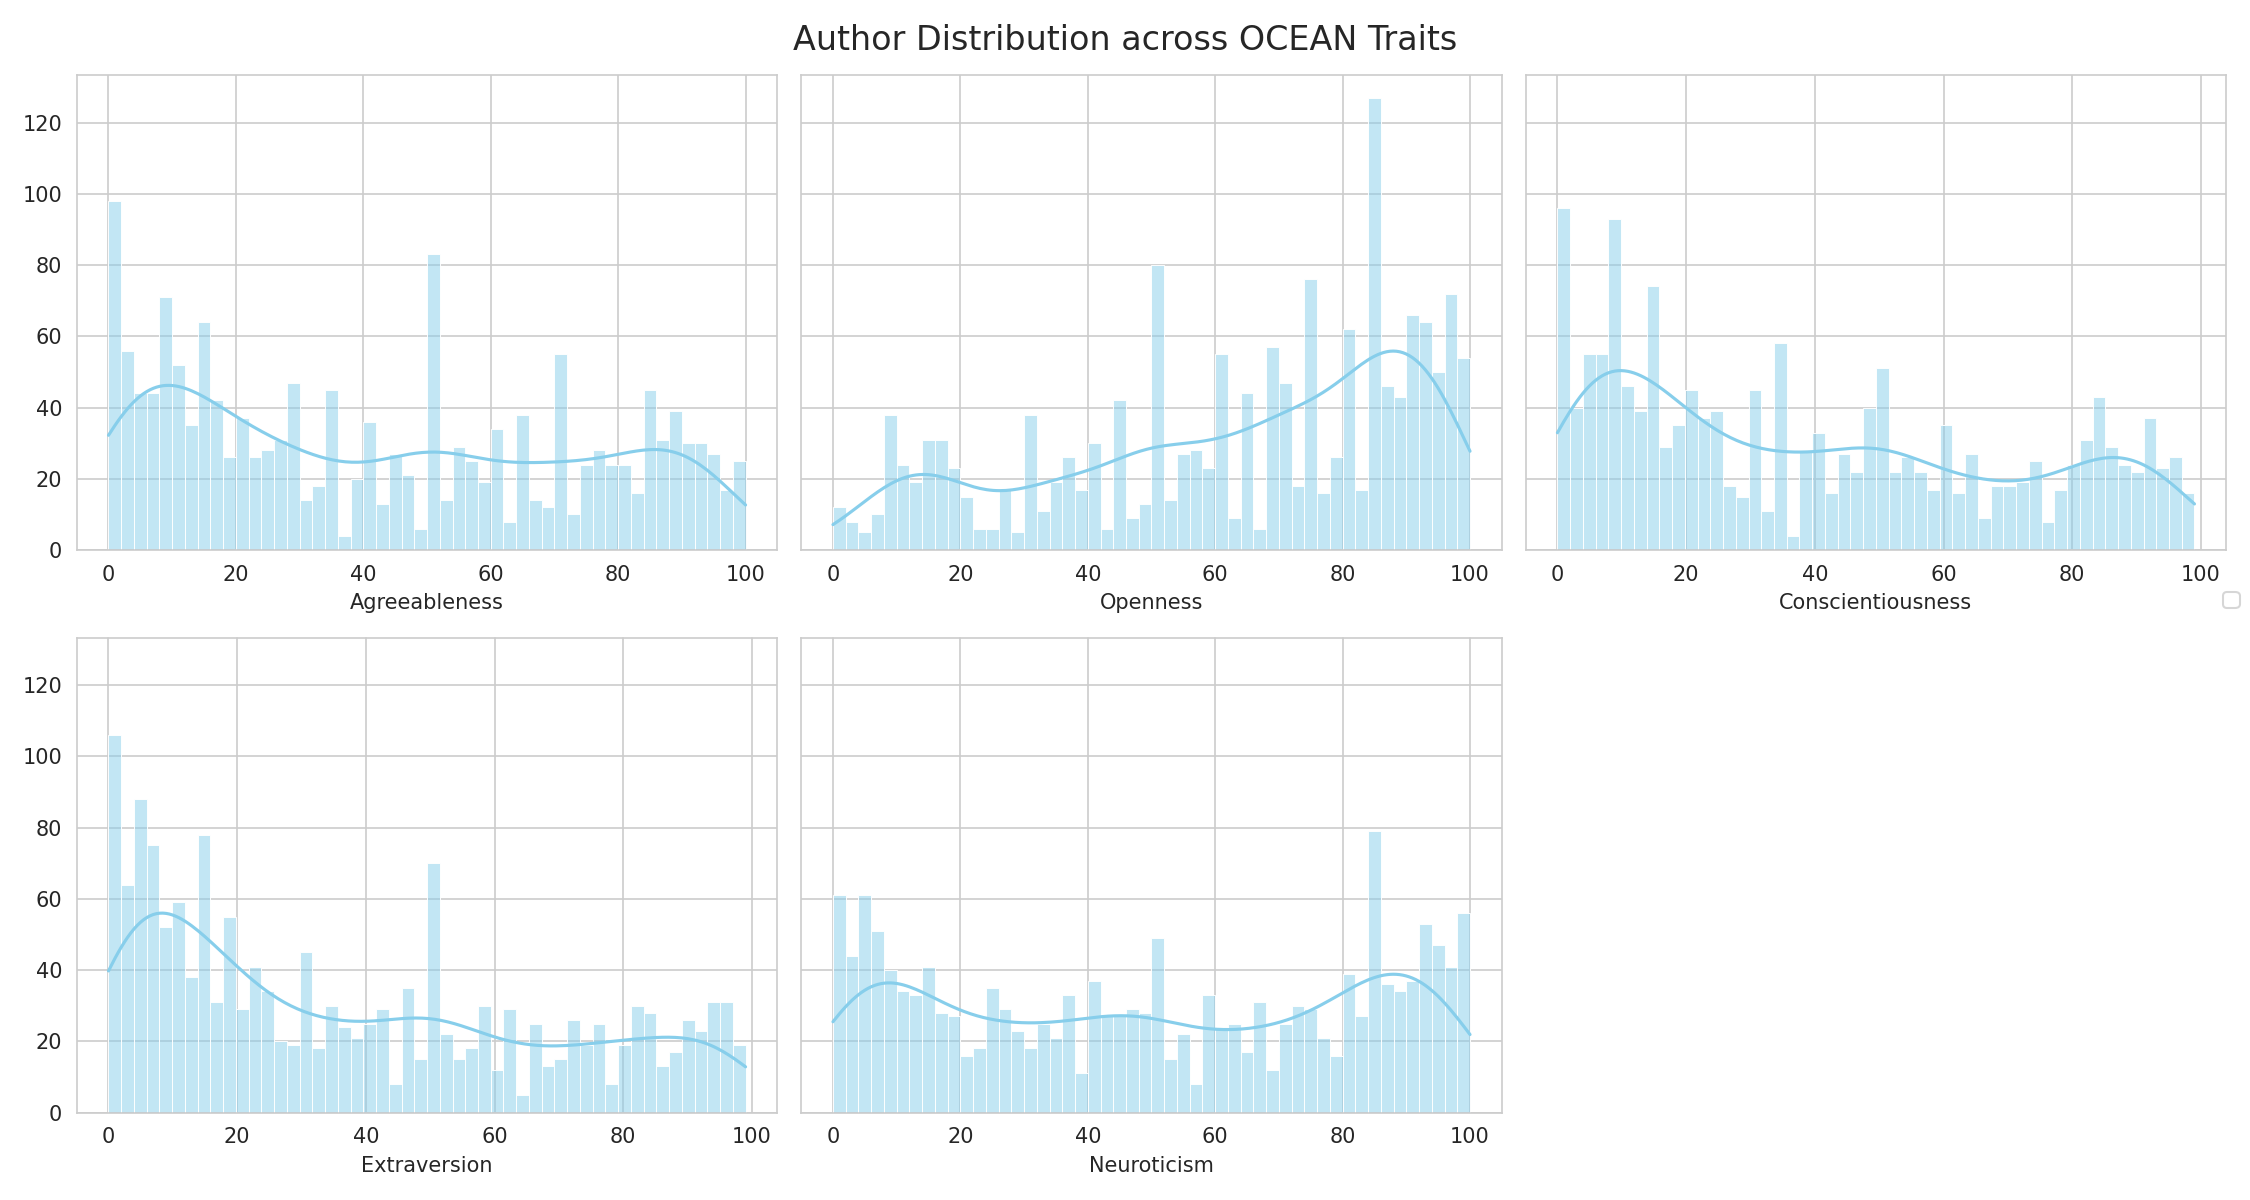
\includegraphics[width=0.8\textwidth]{img/data_eda/1_distribution_of_personality_scores.png}
    \caption{Author count distribution across OCEAN traits | PANDORA}
    \label{fig:author_traits_dist_pandora}
\end{figure}

\begin{figure}[H]
    \centering
    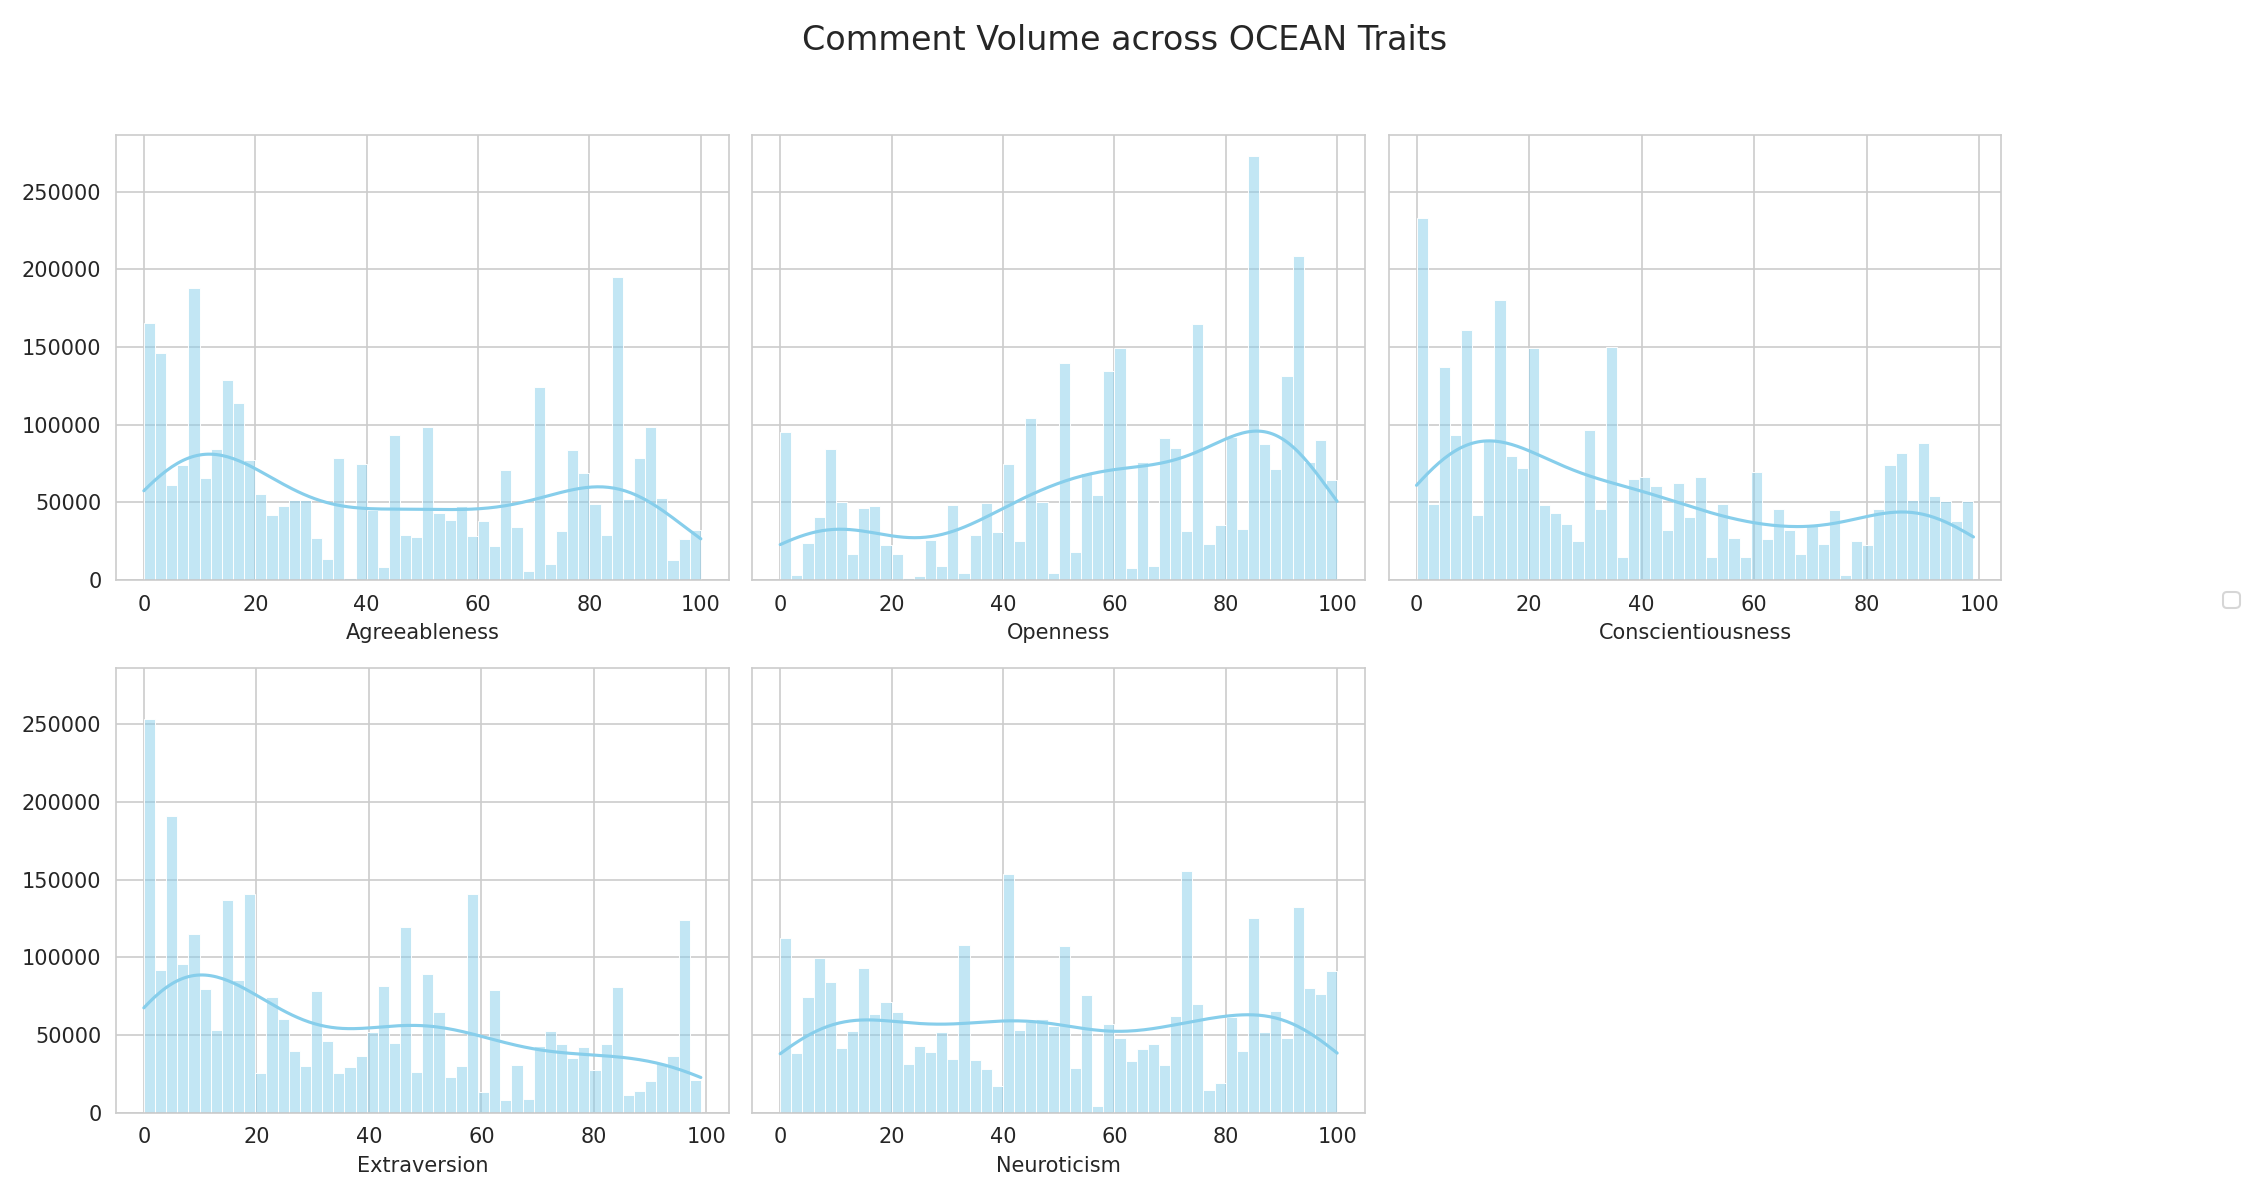
\includegraphics[width=0.8\textwidth]{img/data_eda/2_comment_volume_vs_trait.png}
    \caption{Comment volume across OCEAN traits | PANDORA}
    \label{fig:comment_vol_ocean_pandora}
\end{figure}

\begin{figure}[H]
    \centering
    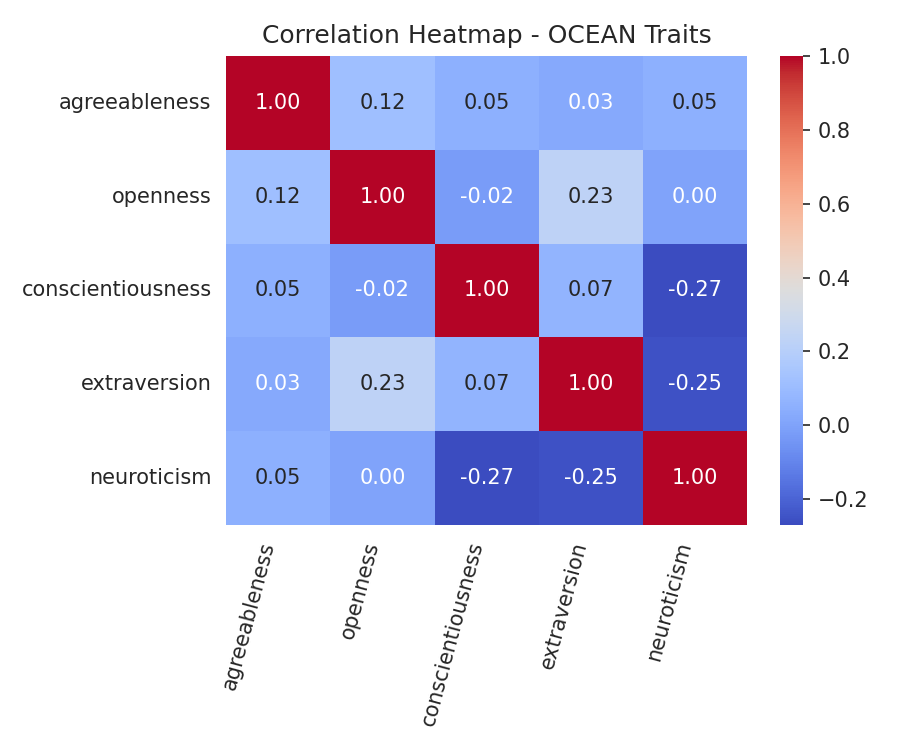
\includegraphics[width=0.8\textwidth]{img/data_eda/3_ocean_trait_correlation.png}
    \caption{OCEAN traits correlation heatmap | PANDORA}
    \label{fig:ocean_trait_correlation_pandora}
\end{figure}

The PANDORA data processing flowchart (Figure \ref{fig:pandora_flowchart}) illustrates the multi-step preprocessing pipeline that was used to get the PANDORA dataset ready for fine-tuning. Using tools like ftfy, comments were first loaded, cleaned to eliminate HTML tags and URLs, and then standardized by eliminating extra whitespace and fixing encoding problems. Only comments from authors who had complete OCEAN trait profiles in the author profiles table were kept, thanks to an important filtering step. Finding common authors who appeared in both the author profiles and comments tables allowed for this to be accomplished.

\begin{figure}[H]
    \centering
    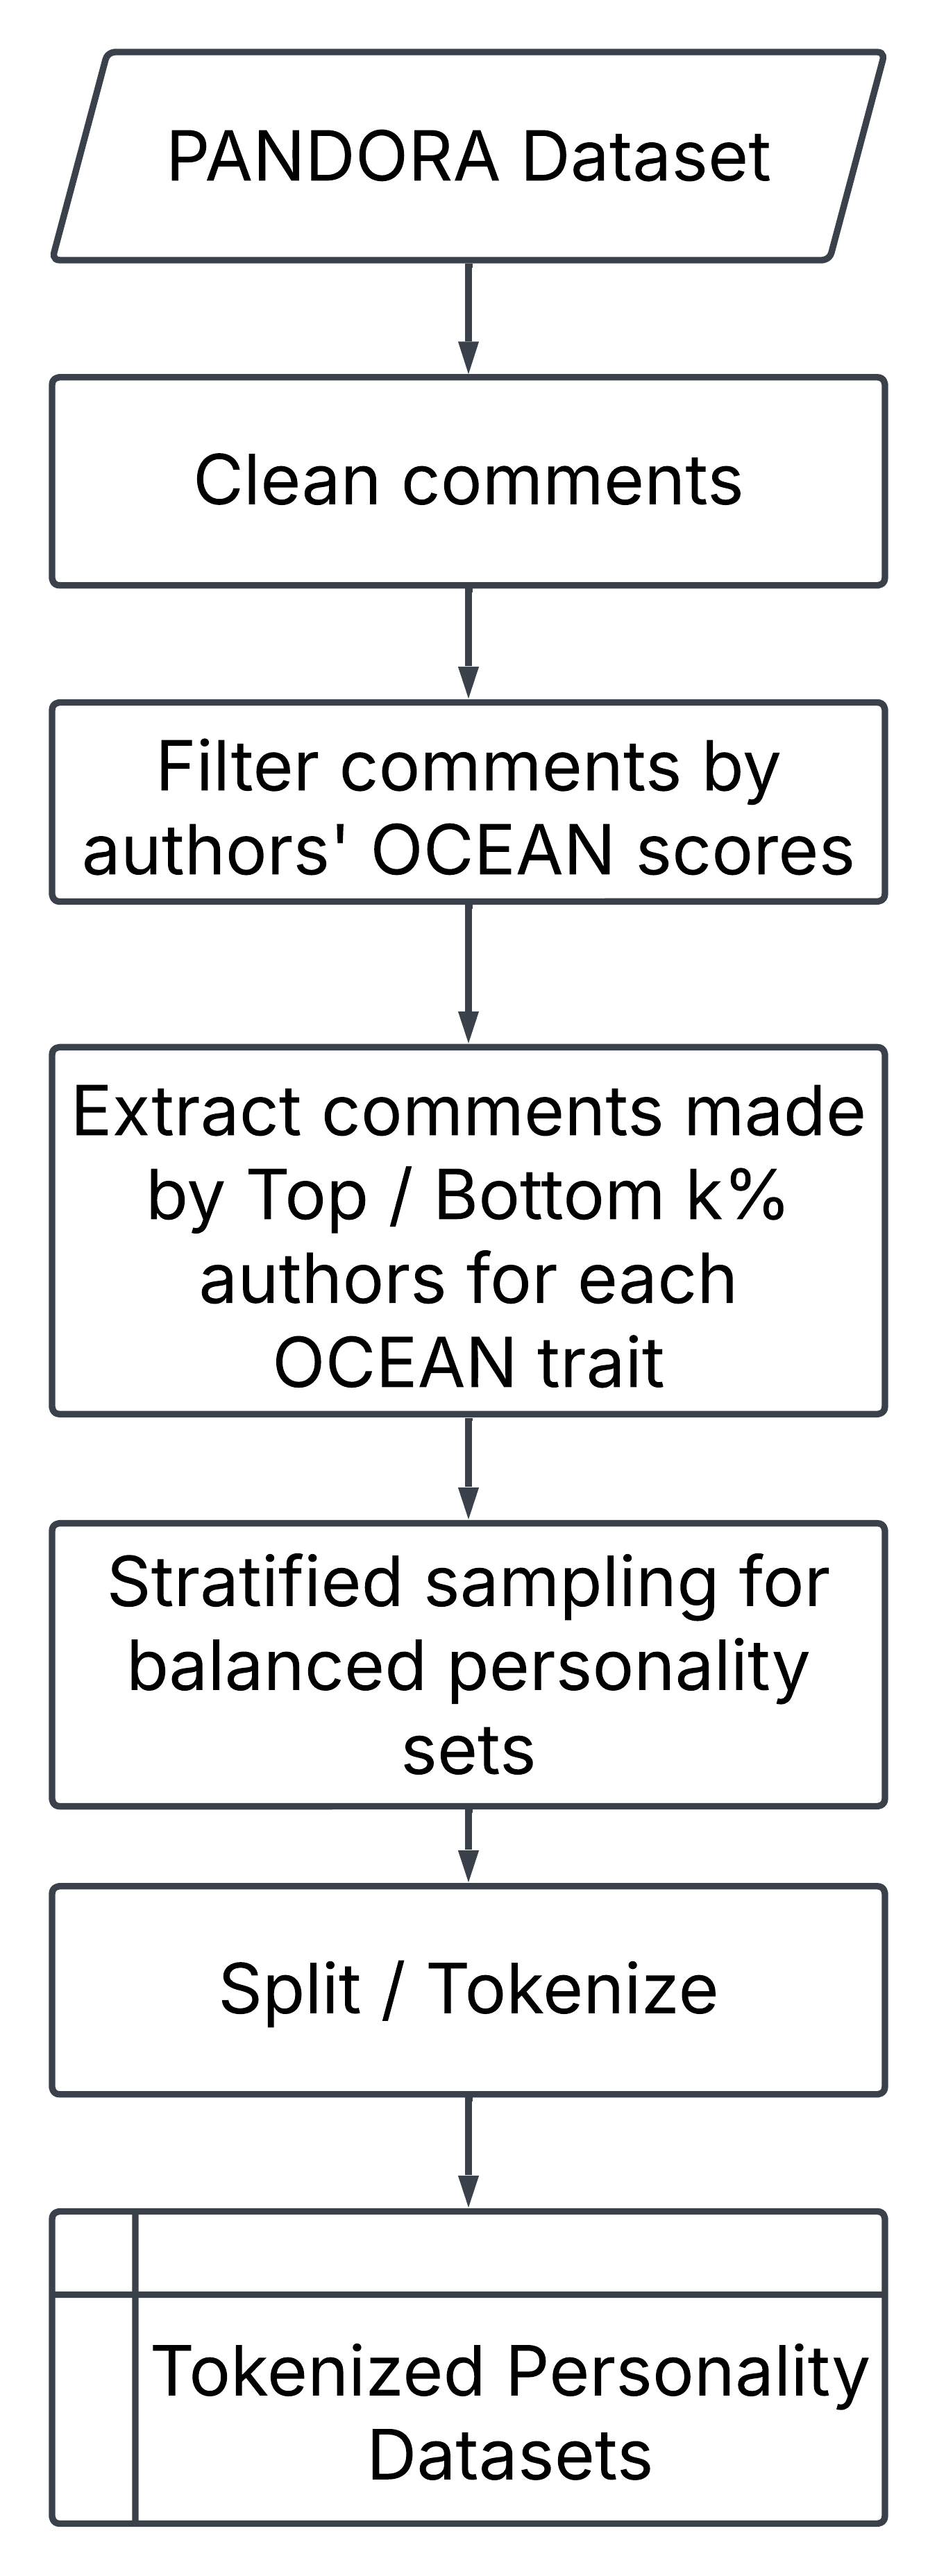
\includegraphics[width=0.3\textwidth]{img/pandora_flowchart.png}
    \caption{Data preparation process for Pandora dataset}
    \label{fig:pandora_flowchart}
\end{figure}

Finding authors who displayed extreme manifestations of each OCEAN trait was the main tactic used to create personality-specific data splits. Authors were ranked according to their scores for each of the five OCEAN traits. We extracted comments from authors who fell into the top k\% (high trait expression) and bottom k\% (low trait expression) categories. Each trait and extremity (e.g., agreeableness-top-5, neuroticism-bot-10) has a unique split because the values for \(k\) were selected from the set \(\{5\%, 10\%, 15\%\}\).

The created trait splits were balanced to guarantee comparability between experiments and to keep dataset size from acting as a confounding factor. We calculated the number of comments in the smallest split (across all traits and both top/bottom conditions for that k) for each k value (5, 10, 15). Then, using random sampling with a fixed seed for reproducibility, all other splits for that same k value were downsampled to match this minimum comment count. For instance, this procedure guarantees that the number of comments in all "bottom-5" splits and all "top-5" splits (Openness-top-5, Conscientiousness-top-5, etc.) is the same. In order to attribute observed variations in model behavior to the trait content of the data rather than the number of training examples, this balancing is essential. Figure \ref{fig:pandora_splits_ocean_heatmap}, which displays the average OCEAN profile for authors contributing to each particular data split (e.g., the average Openness, Conscientiousness, Extraversion, Agreeableness, and Neuroticism scores for authors in the "Openness-top-5" split), visualizes the assumed ground truth OCEAN scores for authors within each of these final balanced splits (based on Mean OCEAN scores of authors across Pandora splits.png).

\begin{figure}[H]
    \centering
    \includegraphics[width=1.0\textwidth]{img/data_eda/10_pandora_splits_heatmap_ground_truth.png}
    \caption{Average OCEAN profile for authors contributing to each particular data split | Ground Truth}
    \label{fig:pandora_splits_ocean_heatmap}
\end{figure}

\subsubsection{Emotion: TweetEval-Emotion}
% Core Theme: Source and Characteristics of the TweetEval-Emotion Dataset
The 'emotion' subset of the TweetEval dataset was used for emotion-driven fine-tuning \cite{barbieri_tweeteval_2020}. The "emotion" subset of the benchmark suite TweetEval, which consists of seven diverse NLP tasks unique to Twitter, is based on the SemEval-2018 Task 1 (Affect in Tweets) dataset, which is concerned with multi-label emotion classification. Eleven emotions have labels in the original dataset. To fit the Positive and Negative Affect Schedule - Expanded Form (PANAS-X) inventory, which is used for assessment, a particular subset of these emotions was chosen for this thesis. Figure \ref{fig:tweeteval_flowchart} shows the TweetEval-Emotion data processing pipeline (based on TweetEval\_data\_pipeline.png).

\begin{figure}[H]
    \centering
    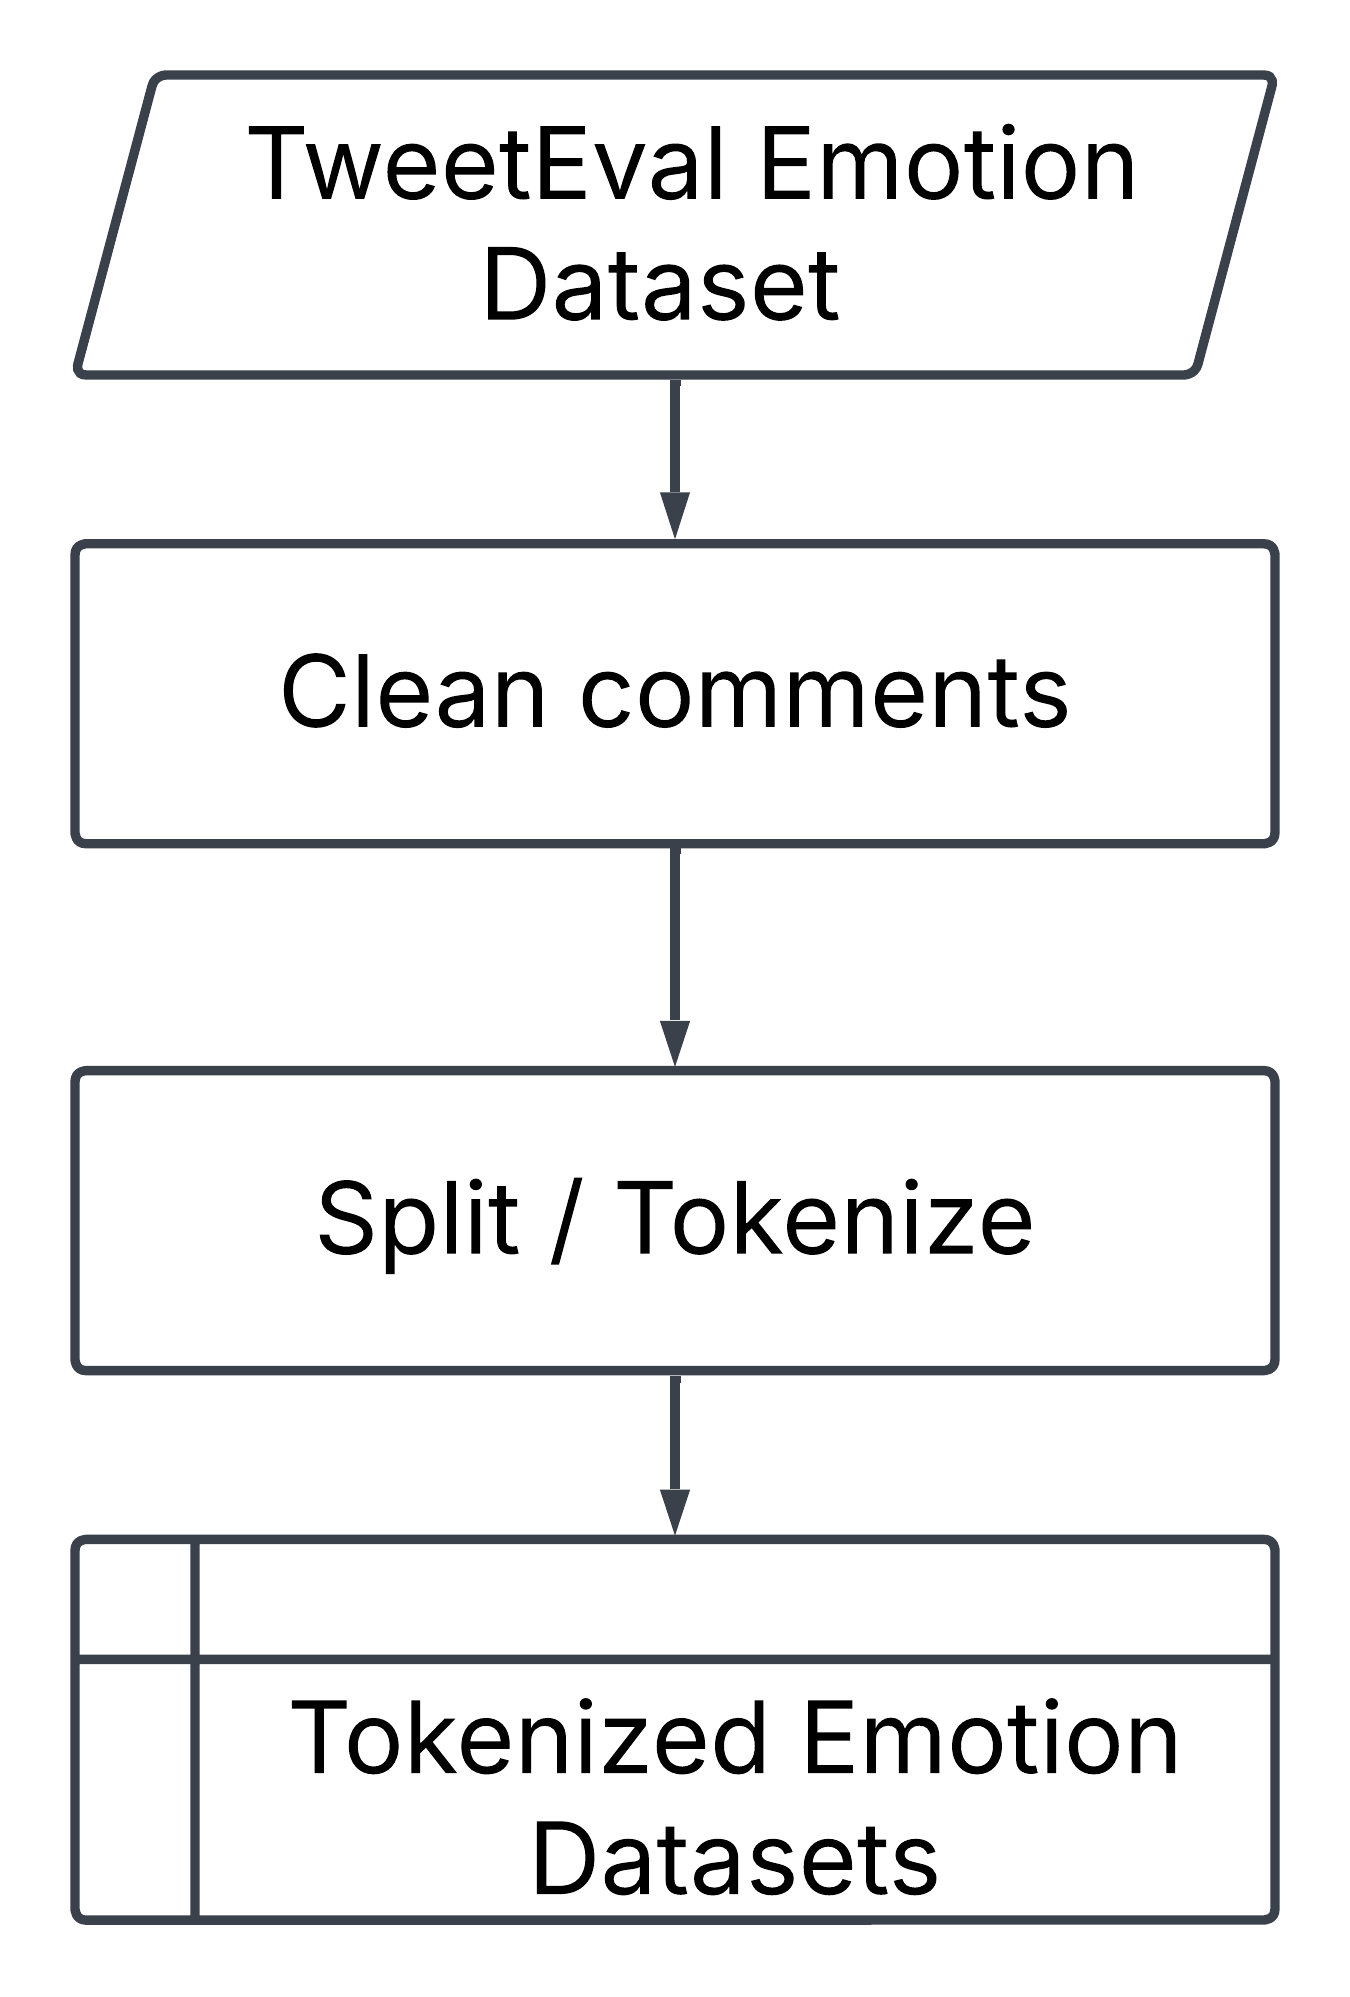
\includegraphics[width=0.3\textwidth]{img/emotion_flowchart.png}
    \caption{Data preparation process for TweetEval-Emotions dataset}
    \label{fig:tweeteval_flowchart}
\end{figure}

In order to preprocess the TweetEval 'emotion' data (train, validation, and test splits combined), "@user" instances were eliminated, and HTML entities (such as \textit{\&amp};) were resolved to "and". Four different emotion-specific data splits were created by extracting the comments associated with "anger" (label 0), "joy" (label 2), "sadness" (label 3), and "optimism" (label 1) from the original emotion labels. The subscales of the PANAS-X inventory that were used for evaluation served as a guide for this selection, which focused on items associated with these fundamental affective states. Figure \ref{fig:tweeteval_emotion_dist} (based on TweetEval Emotion Label Distribution.png) displays the distribution of comments across these chosen emotion labels in the original TweetEval-Emotion dataset. Since the main objective was to capture the linguistic expression of each distinct emotion as represented in the dataset, these emotion splits were not balanced by downsampling, in contrast to the PANDORA splits.

\begin{figure}[H]
    \centering
    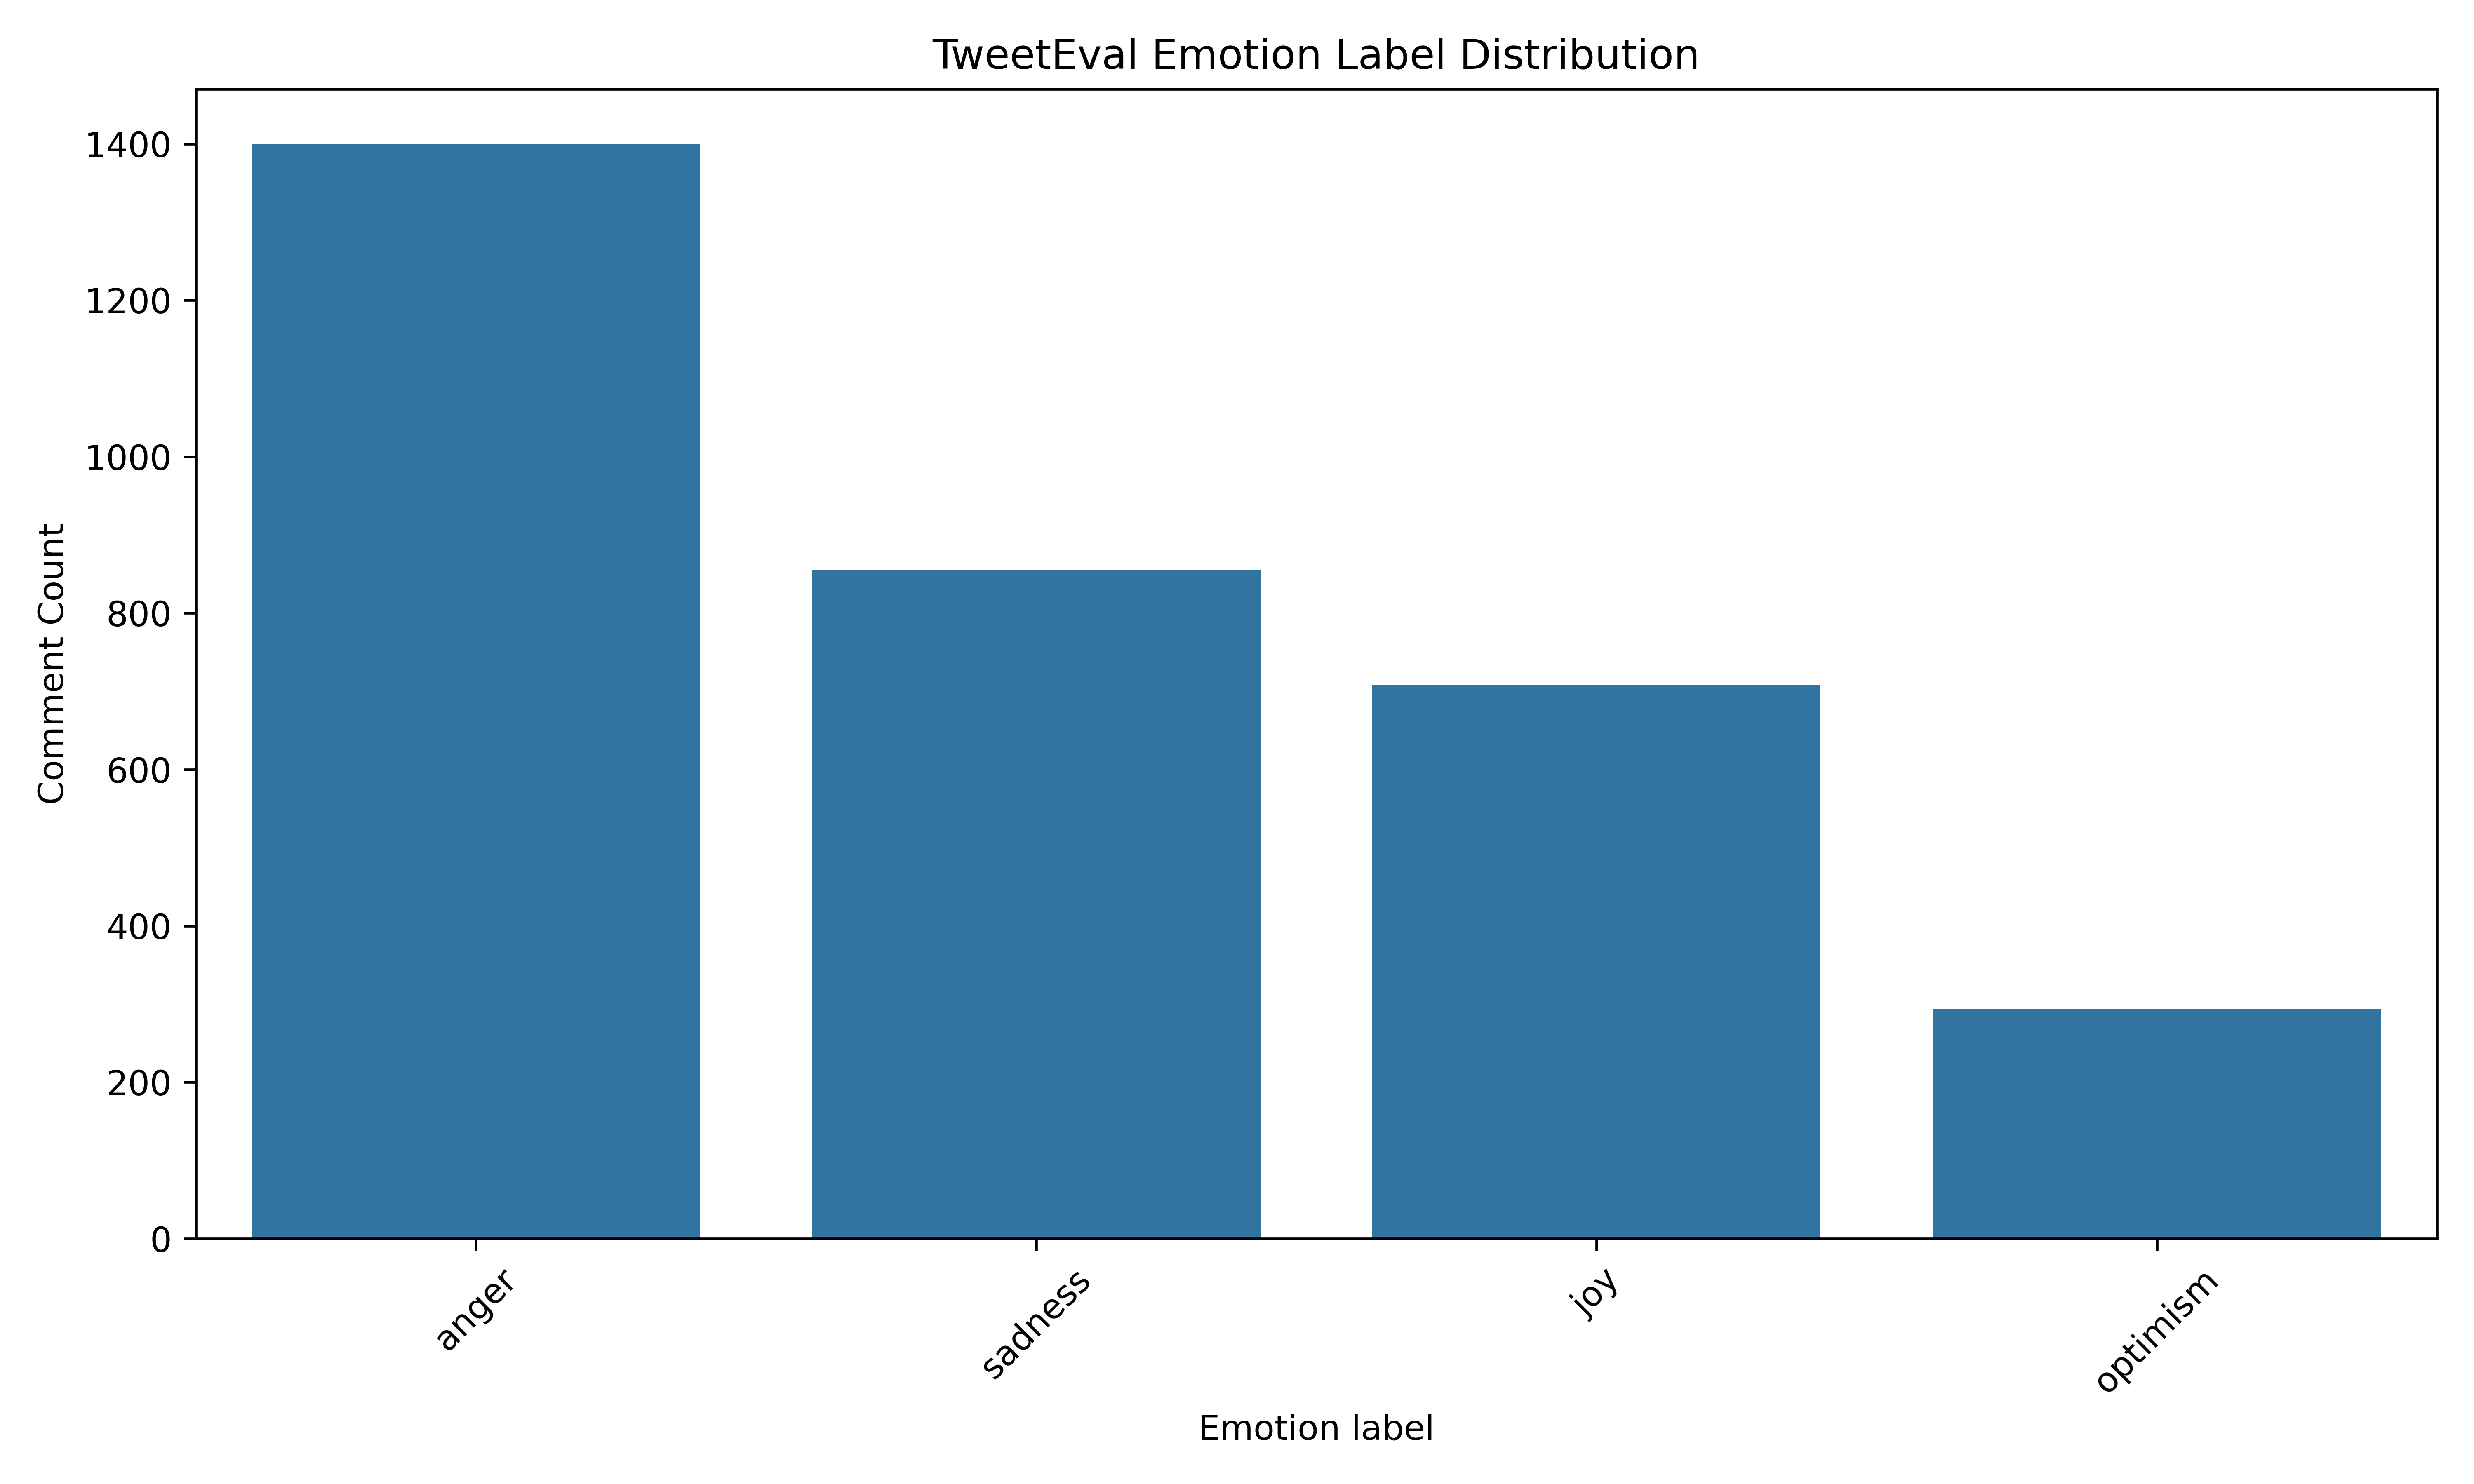
\includegraphics[width=0.8\textwidth]{img/data_eda/9_emotion_barplot.png}
    \caption{Data preparation process for TweetEval-Emotions dataset}
    \label{fig:tweeteval_emotion_dist}
\end{figure}

\subsection{Model Selection \& Fine-tuning Strategies}

\subsubsection{Autoregressive LMs}
GPT-2 (more especially, the 117M parameter version, which becomes 124M with embeddings) is the main language model utilized for all experiments in this thesis. This decision was influenced by multiple factors. First off, GPT-2 is easier to experiment with within the usual academic research constraints due to its smaller size when compared to modern multi-billion parameter models. This allows for more fine-tuning runs and evaluations. Second, the findings are applicable to the larger class of generative language models because its autoregressive Transformer architecture is typical of many contemporary LLMs. Thirdly, previous research has thoroughly examined GPT-2, including studies of its emergent properties and fine-tuning behavior, which offers a rich context for comparing and interpreting findings \cite{caron_manipulating_2023,jiang_evaluating_2023}. Lastly, the experimental pipeline can be quickly prototyped and implemented thanks to its compatibility with well-known libraries like PEFT and Hugging Face Transformers.

\subsubsection{LoRA (PEFT) Configurations \& Scaling}
The GPT-2 model was adjusted to the personality and emotion-specific data splits using two different fine-tuning techniques. The first approach, which acts as a baseline, entails completely adjusting every model parameter for every data split. This strategy exemplifies the conventional approach to task adaptation.
\\
Low-Rank Adaptation (LoRA), a well-known PEFT technique, is employed in the second strategy \cite{hu_lora_2021}. LoRA works by injecting trainable low-rank decomposition matrices into designated Transformer architecture layers and freezing the pre-trained model weights. Compared to full fine-tuning, this offers computational and storage efficiency by drastically reducing the number of trainable parameters \cite{houlsby_parameter-efficient_2019,lialin_scaling_2023}. The Hugging Face PEFT library was used to integrate the LoRA adapters.
\\
Unless otherwise noted, baseline and LoRA experiments were conducted using a common set of fine-tuning hyperparameters to guarantee experiment comparability. For a Causal Language Modeling (CLM) goal, the models were adjusted. Before actual training started, the training script adjusted the initial learning rate, which was set at 1×10−5. An effective batch size of 256 was achieved by using a batch size of 16 and setting gradient accumulation steps to 16. Every model underwent three epochs of training. To potentially stabilize training and enhance generalization, stochastic weighted averaging (SWA) was used. This can also lessen the need for intricate learning rate schedulers \cite{izmailov_averaging_2019}.
\\
For all experiments employing LoRA, a consistent configuration for the LoRA adapters was maintained. This configuration, as implemented via the PEFTManager class, includes:
\begin{itemize}
    \item \textbf{LoRA Rank (r)}: 8. This parameter specifies the rank of the decomposition matrices (A and B), directly influencing the number of trainable parameters in the adapter. A rank of 8 offers a balance between parameter efficiency and adaptive capacity.
    \item \textbf{LoRA Alpha ($\alpha$)}: 16. This scaling factor adjusts the magnitude of the LoRA update. It is often set relative to the rank; here, $\alpha = 2r$.
\item \textbf{LoRA Dropout}: 0.1. A dropout rate of 10\% applied to the LoRA layers during training to mitigate overfitting.
    \item \textbf{Target Modules}: "all-linear". LoRA adapters were applied to all linear layers within the GPT-2 model architecture. This comprehensive application aims to allow adaptation across various model components.
    \item \textbf{Task Type}: "CAUSAL\_LM". This specifies the task for which LoRA is configured, aligning with the fine-tuning objective.
    \item \textbf{Fan-in/Fan-out}: Enabled. This setting ensures correct scaling of weights for certain architectures, though its impact on GPT-2 with "all-linear" targeting might be minimal.
    \item \textbf{Initialization of LoRA Weights}: True (default). LoRA weights (matrices A and B) were initialized using the default method provided by the PEFT library, typically involving Gaussian initialization for A and zeros for B, ensuring that the LoRA path initially has no effect on the model's output \cite{hu_lora_2021}.
\end{itemize}
During the evaluation phase for LoRA-adapted models, the impact of the LoRA adapters was systematically varied by applying a range of scaling factors to the LoRA weights. The scaling factors tested were:
\begin{center}
\begin{minipage}{0.9\linewidth}
\centering
\texttt{-25, -20, -15, -12.5, -10, -7.5, -5, -2.5, -1, -0.5, -0.1, 0, 0.1, 0.5, 1, 2.5, 5, 7.5, 10, 12.5, 15, 20, 25}
\end{minipage}
\end{center}
\\
This makes it possible to investigate the effects of increasing or decreasing the LoRA influence on the model's expression of personality or emotion traits (Hypothesis H2). Figure \ref{fig:experimental_pipeline} shows the overall fine-tuning and evaluation pipeline (based on Experimental\_Pipeline\_Diagram.png).

\subsubsection{Task Arithmetic Vector Algebra}
To examine the effects of combining learned trait-specific adaptations, task arithmetic experiments were created (Hypothesis H3). This entails applying arithmetic operations to the "task vectors" that are obtained from the refined models \cite{ilharco_editing_2023}. This thesis investigates a particular type of task arithmetic by combining LoRA adapters that have been fine-tuned on one type of data (such as a TweetEval-Emotion split) with a baseline model that has been fine-tuned on another type of data (such as a PANDORA personality split), or vice versa.
\\
The procedure involves:
\begin{enumerate}
    \item Loading a fully fine-tuned baseline model (e.g., GPT-2 fine-tuned on agreeableness-top-5).
\item Setting up this baseline model with a LoRA configuration (as previously mentioned, adding new, untrained LoRA matrices A and B and freezing its initial weights).
\item loading the weights of the LoRA adapters (matrices A and B) that were trained on a different data split (for example, the GPT-2 LoRA adapters that were optimized on the anger emotion split). Step 1 involves loading these LoRA weights into the baseline model's LoRA layers.
\end{enumerate}
\\
This effectively overlays a model that has already been specialized for one task or trait with the LoRA adaptation that was learned for that task or trait. The influence of the LoRA adapter is then adjusted using the same range of scaling factors as in the standard LoRA experiments, and the combined model is subsequently assessed using the psychometric inventories. This makes it possible to examine the effects of increasing or decreasing (through negative scaling) the "emotion task vector" (represented by the LoRA weights) on the base model's "personality profile" and vice versa.

\subsection{Evaluation Instruments \& Prompting Protocol}
Standardized psychometric inventories are used to evaluate personality and emotion traits in the refined LLMs. To administer these inventories to the models and measure their responses, a unique prompting and scoring pipeline was created.

\subsubsection{BFI-10 \& IPIP-120}
For assessing the Big Five OCEAN personality traits, two instruments are used:
\begin{enumerate}
\item \textbf{BFI-10 (Big Five Inventory-10)}: The purpose of this short 10-item test is to evaluate the five major areas of personality \cite{rammstedt_big_2014}. Two items, one positively keyed and one negatively keyed, are used to measure each of the following traits: neuroticism, agreeableness, extraversion, conscientiousness, and openness. Although it offers a less detailed measure than longer inventories, its conciseness makes it appropriate for quick evaluation.
\item \textbf{IPIP-120 (item version of the International Personality Item Pool 120)}: The five broad domains and thirty specific facets of the Five-Factor Model are measured by this more extensive public-domain inventory, which has four items per facet and six facets per domain \cite{johnson_measuring_2014,maples_test_2014}. According to Johnson (2014), the IPIP-NEO-120 seeks to replicate the proprietary NEO PI-R's constructs. A more thorough, facet-level examination of personality is made possible by its inclusion.
\end{enumerate}

\subsubsection{PANAS-X}
The Positive and Negative Affect Schedule - Expanded Form (PANAS-X) is used to measure emotional states \cite{david_watson_panas-x_1994}. In addition to more specialized emotions, the PANAS-X evaluates two general higher-order dimensions: Positive Affect (PA) and Negative Affect (NA). A subset of PANAS-X items was chosen for this thesis in order to correspond with the emotion categories found in the TweetEval-Emotion dataset. In particular, words like "determined," "confident," and "strong" were used to conceptualize the emotions of anger, sadness, joy, and optimism. In order to assess the model's current "feeling" state in response to the item, the PANAS-X usually asks respondents to rate the degree to which they have experienced these feelings over a predetermined period of time.

\subsubsection{Custom Likert-scale Scoring Pipeline}
A custom pipeline was developed to administer the inventory items to the LLMs and score their responses. This protocol is designed to elicit responses on a 5-point Likert scale.
\begin{enumerate}
\item \textbf{Quick Construction}: A prompt is created for every item in the inventory. A general question stem (e.g., "How well does the following statement describe you?"), the specific item formatted into a statement (e.g., "STATEMENT: I see myself as someone who is reserved."), and an optional list of the Likert scale anchors (e.g., "Disagree strongly", "Disagree a little", etc.) are all included in this prompt. For every item, two variations are tested: one in which the Likert anchors are explicitly included in the prompt ("include options"), and another in which they are not ("exclude options"). "YOUR RESPONSE: " marks the end of the prompt.
\item \textbf{Generation and Assessment of Responses}: There is no request for the LLM to produce free-form text. Rather, the anchor text is added to the prompt's "YOUR RESPONSE:" section for each of the five Likert anchors. Given the previous prompt context, the model then determines the average negative log-likelihood (average cross-entropy loss) for producing the tokens of that particular anchor. For a particular item, this procedure is repeated for each of the five anchors.
\item \textbf{Probability Conversion}: By applying a softmax function to the negative losses (softmax(−Lanchor)), the average losses for the five anchors are transformed into a probability distribution. The model's preference for each response option is indicated by the probability score that is produced for each of the five Likert scale points. For every item, the sum of these probabilities equals 1.
    \item \textbf{Extraction of Likert Scores}: From this probability distribution, two types of Likert scores are extracted for each item:
\begin{enumerate}
\item \textbf{max}: The Likert scale point (1 to 5) that received the highest probability.
        \item \textbf{weighted}: A continuous score calculated as the weighted sum of the Likert scale points, where each point is weighted by its probability \[\text{weighted\_likert} = \sum_{i=1}^{5} i \, P(\text{anchor}_{i})\].
\end{enumerate}
\end{enumerate}

\subsubsection{Post-Hoc Inventory Scoring and Debiasing}
After obtaining the raw Likert scores for each item from the EvalManager, a subsequent script processes these scores:
\begin{enumerate}
\item \textbf{Reverse Coding} Negatively keyed items are reverse-coded, that is, \(x \mapsto 6 - x\) on a 5-point scale, for inventories such as BFI-10 and IPIP-120. This guarantees that higher scores always correspond to a higher trait level.

\item \textbf{Trait and Facet Score Calculation}:
\begin{itemize}
\item Each of the five OCEAN traits' scores on the BFI-10 are determined by averaging the Likert scores of the two items that correspond to that trait, which may be reverse-coded.
\item The average of the (possibly reverse-coded) Likert scores of the four items that make up each of the 30 facets of IPIP-120 is used to determine scores for each facet. The scores of their six component facets are then averaged to determine the scores for the five broad OCEAN traits.
\item The Likert scores of the items chosen to represent the affective states of anger, sadness, joy, and optimism are averaged for the adapted PANAS-X.
\end{itemize}

\item \textbf{Debiasing Scores in the Pacific Ocean}: The OCEAN trait scores from models tuned on PANDORA data undergo a debiasing step in light of the observed intercorrelations between OCEAN traits in the PANDORA dataset (Figure~\ref{fig:ocean_trait_correlation_pandora}) and the mean OCEAN profiles of the PANDORA splits (Figure~\ref{fig:pandora_splits_ocean_heatmap}).

By taking into consideration the influence of other traits present in the training split, this step seeks to isolate the effect of the target trait. The debiasing process involves fitting a linear regression model in which the ground truth mean scores of all five OCEAN traits for that split predict the model's assessed score for a target trait \(j\), represented by \(Y_j\):
\[
    Y_{\text{adj},j} = Y_{j} - \sum_{k \neq j} \beta_{j,k} X_{k},
\]
where:
\begin{itemize}
        \item \(Y_{j}\) is the model's assessed score on trait \(j\),
        \item \(X_{k}\) is the ground truth mean score of trait \(k\) in the split,
        \item \(\beta_{j,k}\) are the regression coefficients from the linear model.
\end{itemize}

    The resulting \(Y_{\text{adj},j}\) is the residualized (debiased) score, representing the unique contribution of trait \(j\) after accounting for co-occurring traits in the data.
\end{enumerate}

\subsection{Experimental Factors \& Robustness Checks}
To guarantee the validity and robustness of the results, a number of factors are taken into account. In order to fine-tune and account for initialization variability, experiments are carried out using multiple random seeds. It is possible to verify the consistency of personality assessments across various instruments by using two distinct personality inventories (BFI-10 and IPIP-120). A robustness check is built into the evaluation prompting protocol itself, which compares the outcomes of including and excluding Likert options from the prompt. The goal of creating balanced data splits for PANDORA is to account for the effects of dataset size. Another step in identifying real trait effects is the debiasing process for PANDORA scores. Although it is outside the purview of this thesis to fully examine all prompt sensitivities, these steps help to establish a more rigorous methodological approach.


%%%%%%%%%%%%%%%%%%%%% Chapter 6 %%%%%%%%%%%%%%%%%%%%%%
\chapter{Findings}
\thispagestyle{empty}

\subsection{Personality-related Experiments}
\subsubsection{Baseline vs. LoRA Effects Across Inventories}
The purpose of the first set of tests was to determine how full fine-tuning affected the GPT-2 model's perceived personality traits as determined by the BFI-10 and IPIP-120 inventories. This study supports Hypothesis H1, according to which a model would display linguistic patterns and produce responses that are consistent with an amplified expression of a particular personality trait if it were fine-tuned using text data from people who exhibited extreme levels of that trait. The pre-trained GPT-2 model, before any particular personality-driven fine-tuning, serves as the baseline for comparison in these experiments. Following fine-tuning on PANDORA data splits representing the top and bottom 5\%, 10\%, and 15\% of authors for each trait, the results are displayed in figures like Figure \ref{fig:w_i_H1_BFI10_Agreeableness_top}.

\begin{figure}[H]
    \centering
    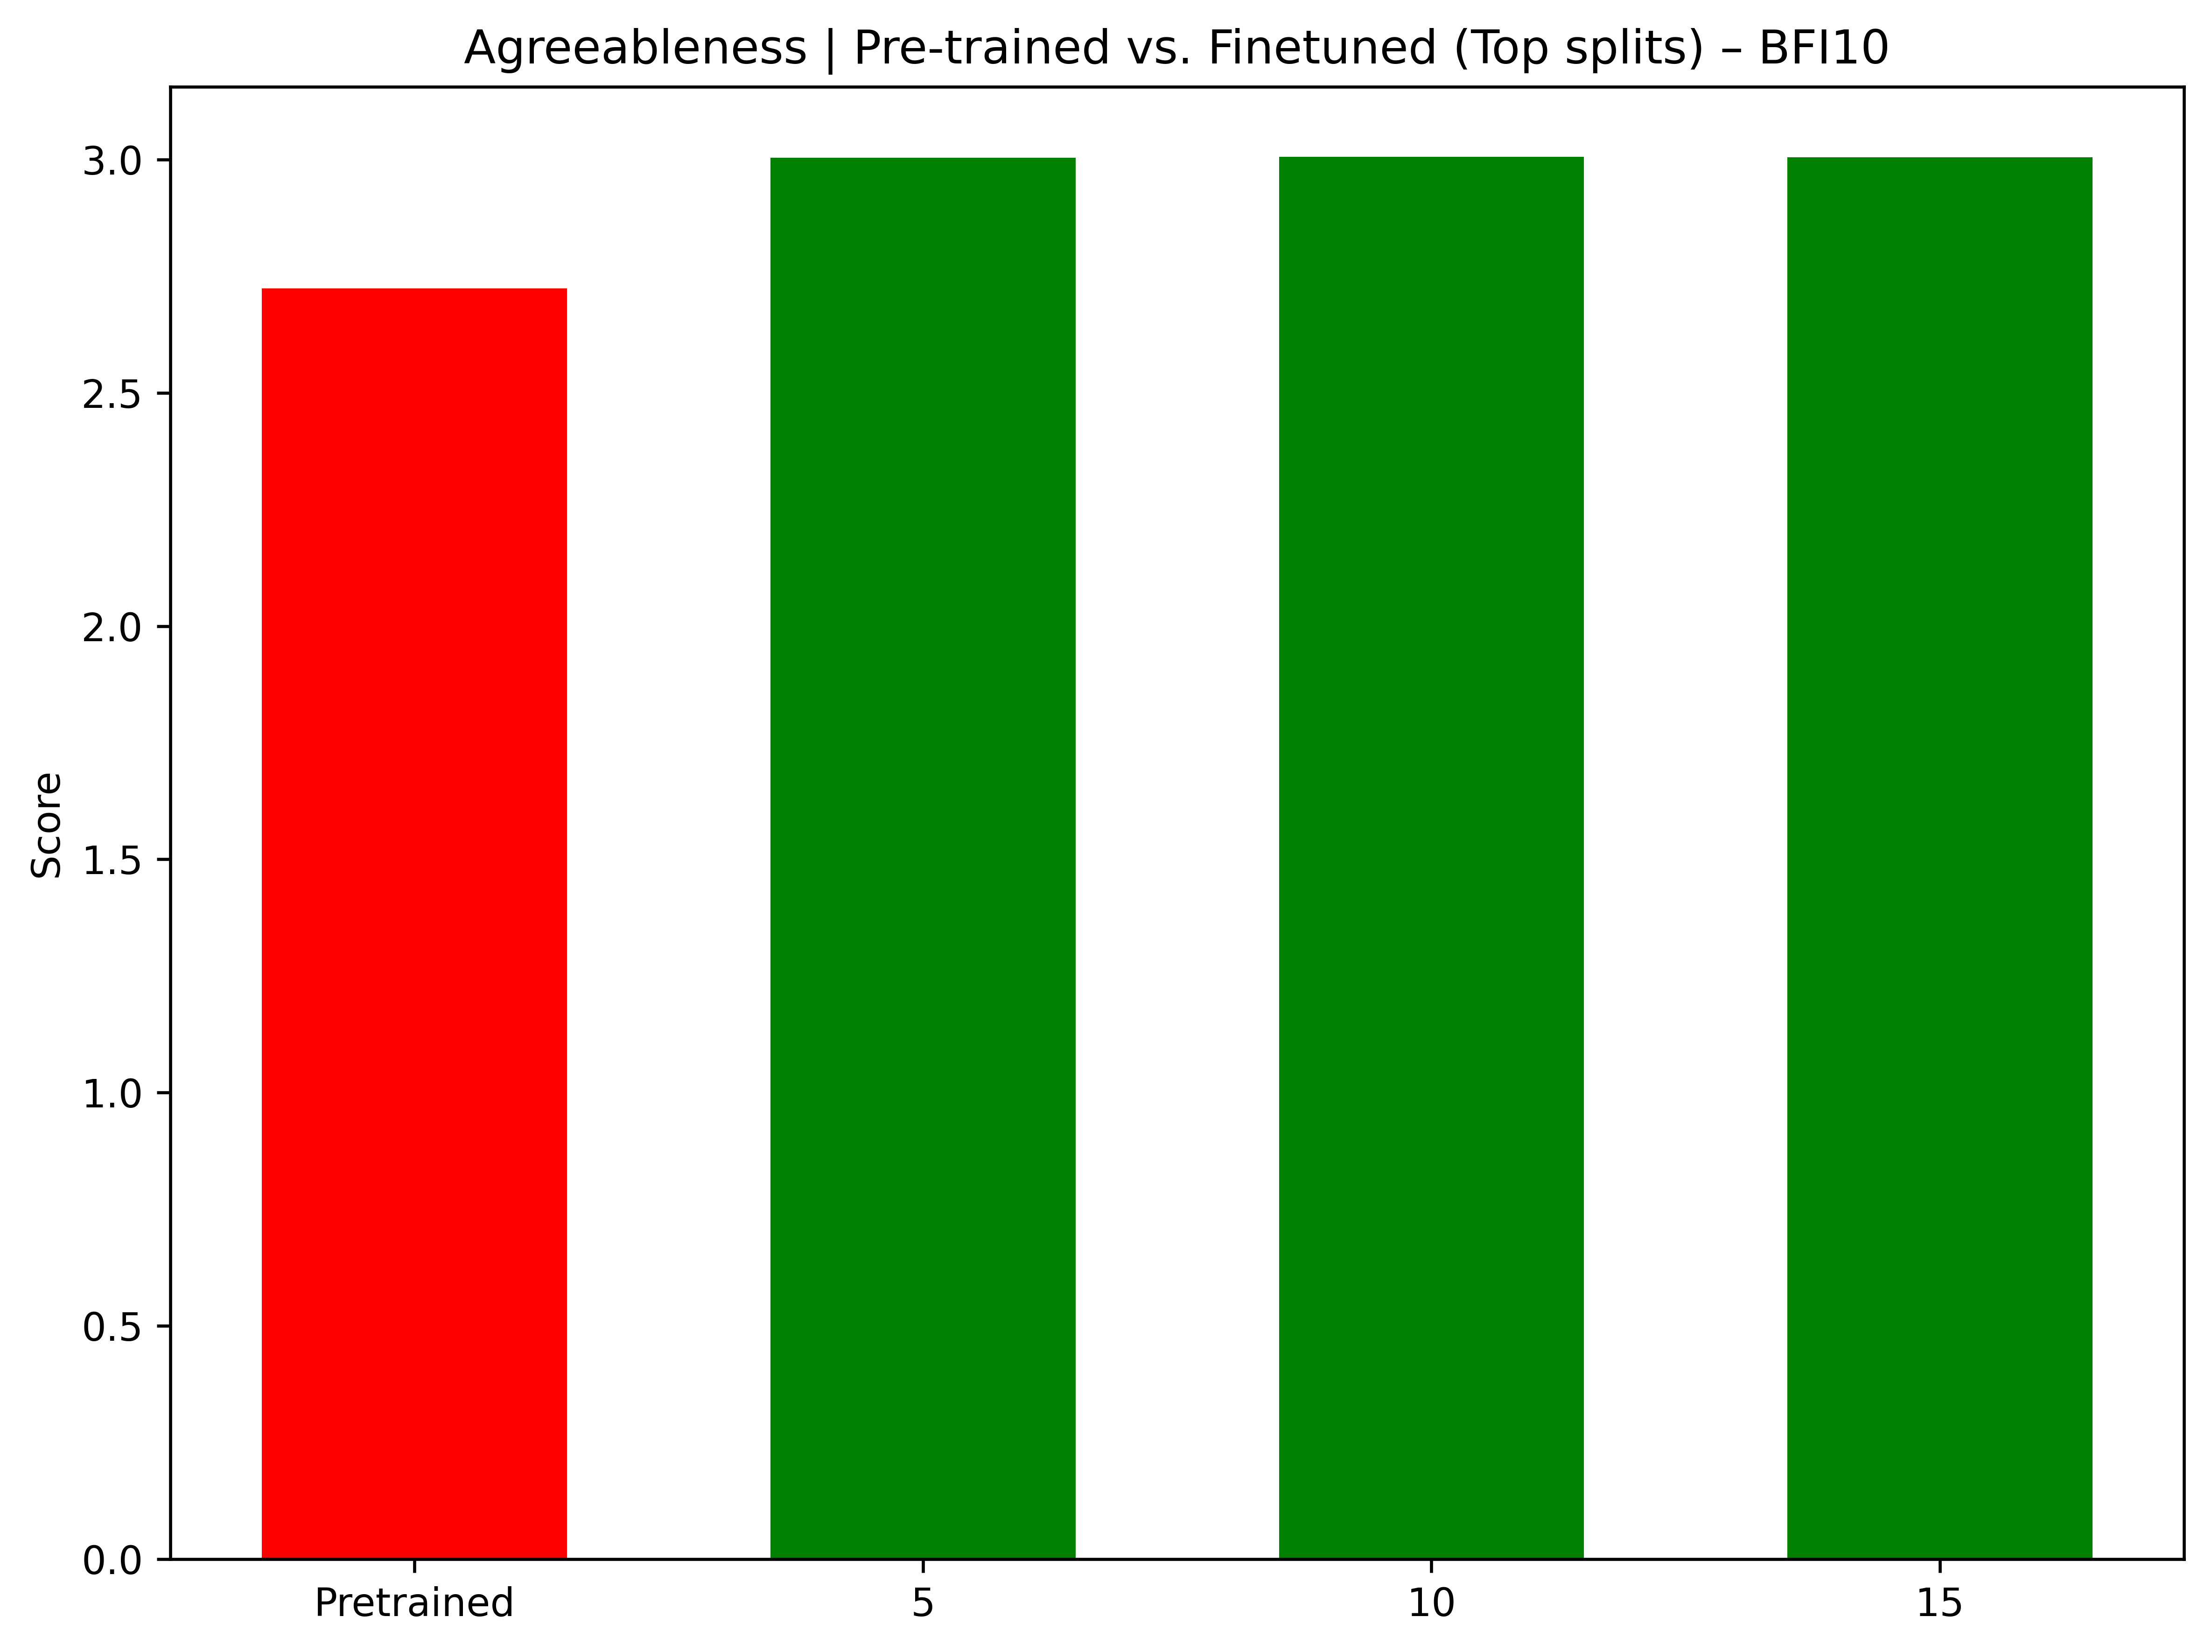
\includegraphics[width=0.8\textwidth]{img/results/w_i_H1_BFI10_Agreeableness_top.png}
    \caption{Conscientiousness scores | Pre-trained vs. Finetuned on top Pandora splits | BFI-10}
    \label{fig:w_i_H1_BFI10_Agreeableness_top}
\end{figure}
\\
The fine-tuning process on PANDORA data splits generally caused shifts in the target personality traits when evaluating with the BFI-10 inventory using weighted Likert scoring and prompts including response options, though the consistency and magnitude varied. For example, the Agreeableness score increased slightly from about 2.85 (pre-trained) to about 2.95-3.00 across the 5\%, 10\%, and 15\% fine-tuned models when the "Agreeableness-top-5\%" split (Figure \ref{fig:w_i_H1_BFI10_Agreeableness_top}) was fine-tuned. On the other hand, compared to the pre-trained model, fine-tuning on "Agreeableness-bottom-5\%" (Figure \ref{fig:w_i_H1_BFI10_Agreeableness_bottom}) resulted in a slight drop in Agreeableness scores, with scores ranging between 2.80 and 2.85.
\\
Although the effect sizes were not always significant, the refined models (green bars) continuously displayed scores that were marginally different from the pre-trained model (red bar), usually in the predicted direction. It is generally expected that LLMs will learn to imitate patterns in their training data \cite{jiang_evaluating_2023, pan_llms_2023, safdari_personality_2023}.

\begin{figure}[H]
    \centering
    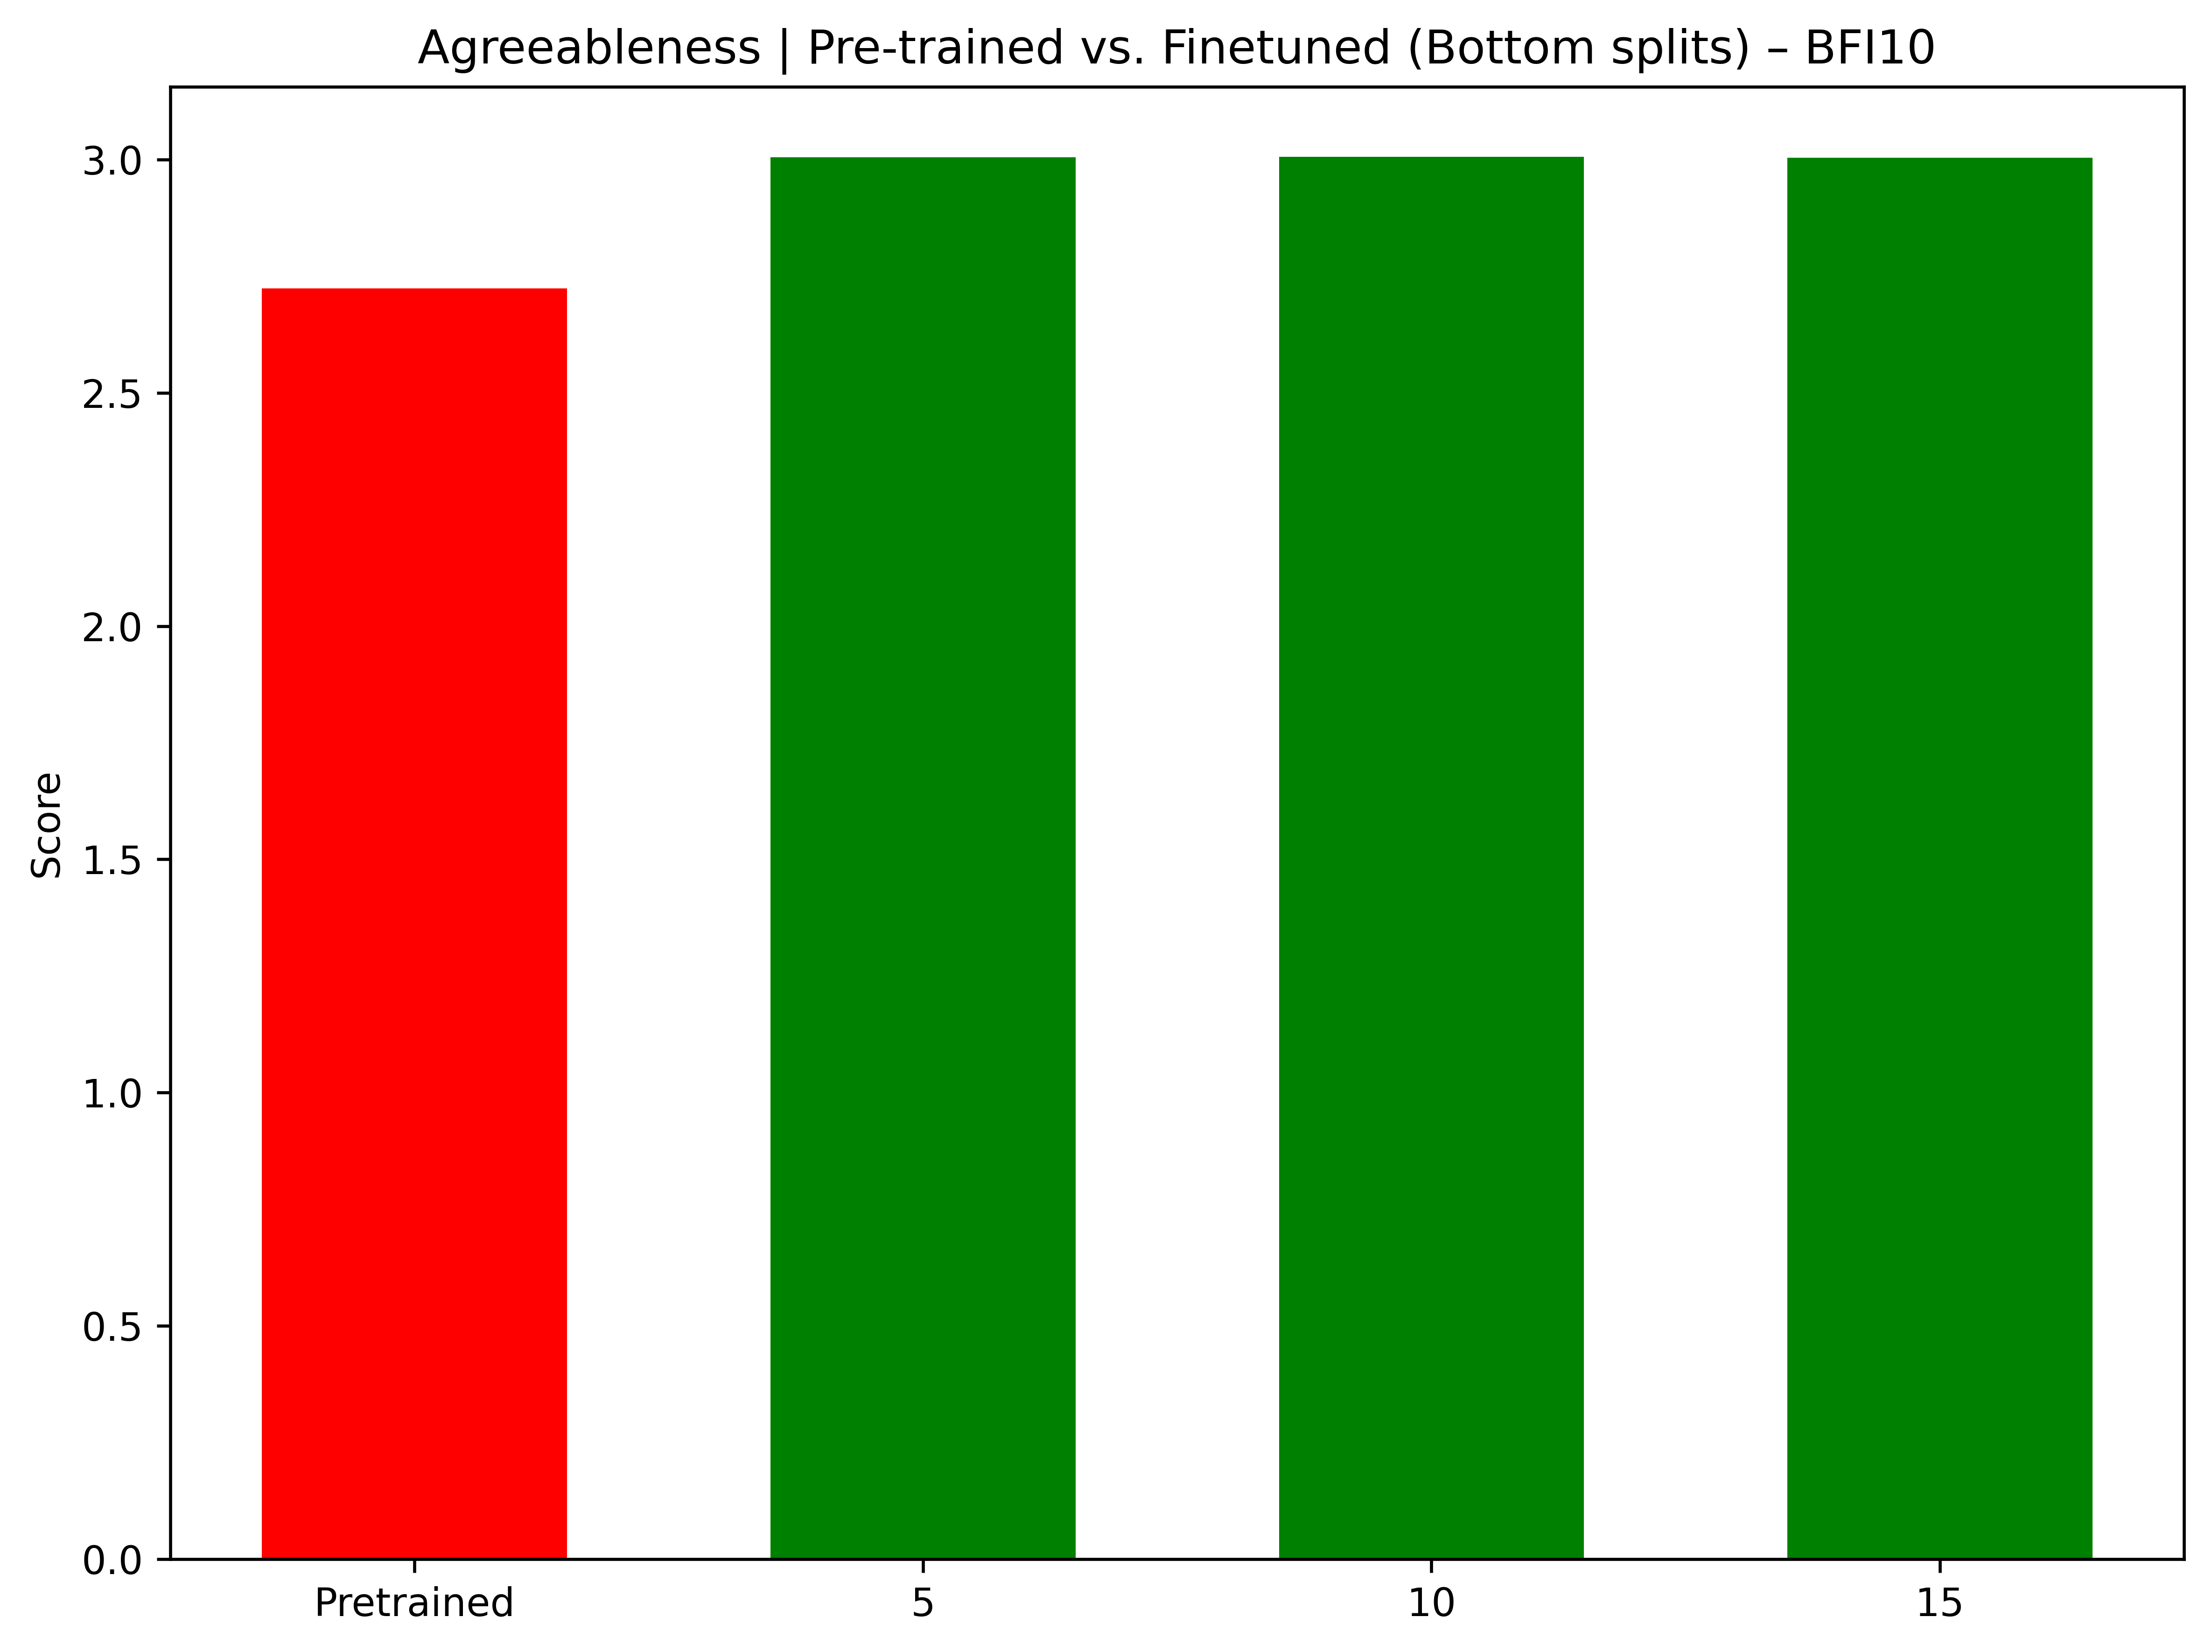
\includegraphics[width=0.8\textwidth]{img/results/w_i_H1_BFI10_Agreeableness_bottom.png}
    \caption{Conscientiousness scores | Pre-trained vs. Finetuned on bottom Pandora splits | BFI-10}
    \label{fig:w_i_H1_BFI10_Agreeableness_bottom}
\end{figure}

\\
Similar patterns were found in the IPIP-120 inventory, which offers a more detailed evaluation. For instance, fine-tuning the "Agreeableness-top-15\%" split (Figure \ref{fig:w_i_H1_IPIP120_Agreeableness_top}) produced an Agreeableness score of about 2.98, which was marginally higher than the score of about 2.92 obtained from the pre-trained model. Adjusting "Agreeableness-bottom-15\%" (Figure \ref{fig:w_i_H1_IPIP120_Agreeableness_bottom}) produced a score of about 2.90, indicating a slight change. When using the IPIP-120 to evaluate the other OCEAN traits, similar patterns of slight, directionally consistent changes were seen (Figures \ref{fig:w_i_H1_IPIP120_Conscientiousness_top} through \ref{fig:w_i_H1_IPIP120_Openness_bottom}). Although the magnitude of change indicates that complete fine-tuning on these PANDORA splits results in relatively subtle changes in the model's overall personality profile as measured by these inventories, the consistency of these findings across various instruments (BFI-10 and IPIP-120) lends some support to H1. For full fine-tuning, the size of the PANDORA split (5\%, 10\%, or 15\%) did not seem to significantly change the results; for a given trait and condition, all three green bars usually displayed scores that were comparable.

\begin{figure}[H]
    \centering
    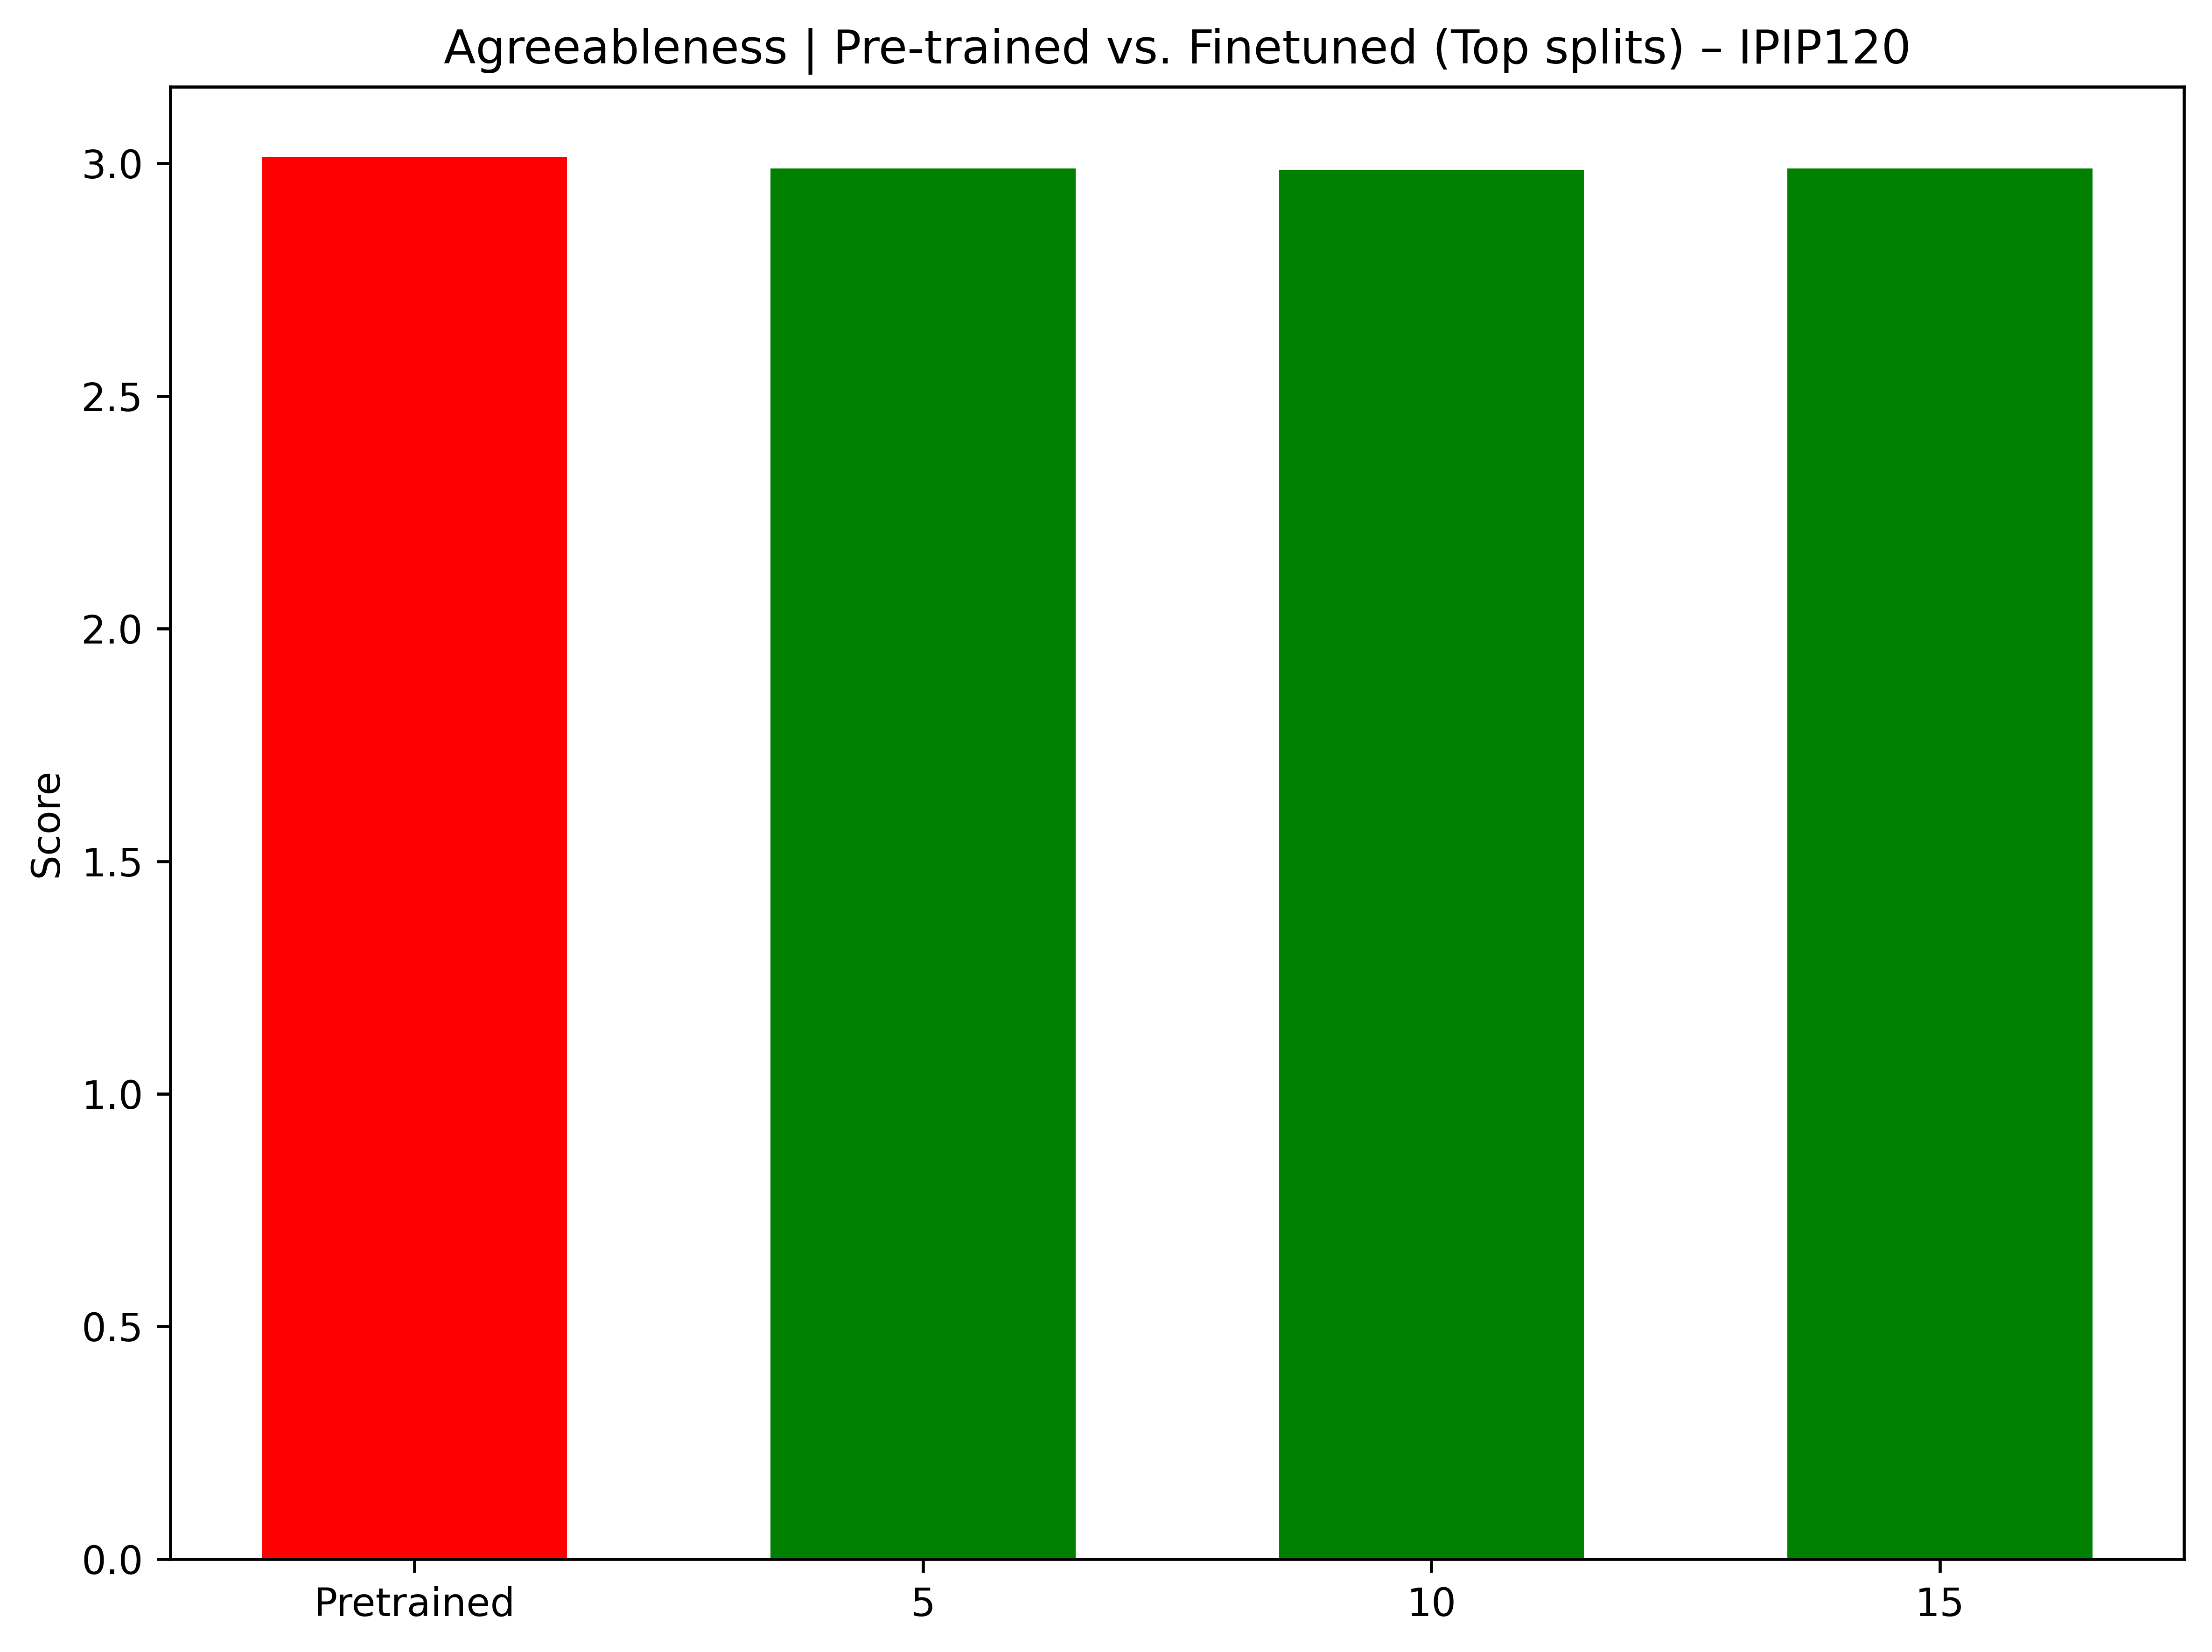
\includegraphics[width=0.8\textwidth]{img/results/w_i_H1_IPIP120_Agreeableness_top.png}
    \caption{Agreeableness scores | Pre-trained vs. Finetuned on top Pandora splits | IPIP-120}
    \label{fig:w_i_H1_IPIP120_Agreeableness_top}
\end{figure}

\begin{figure}[H]
    \centering
    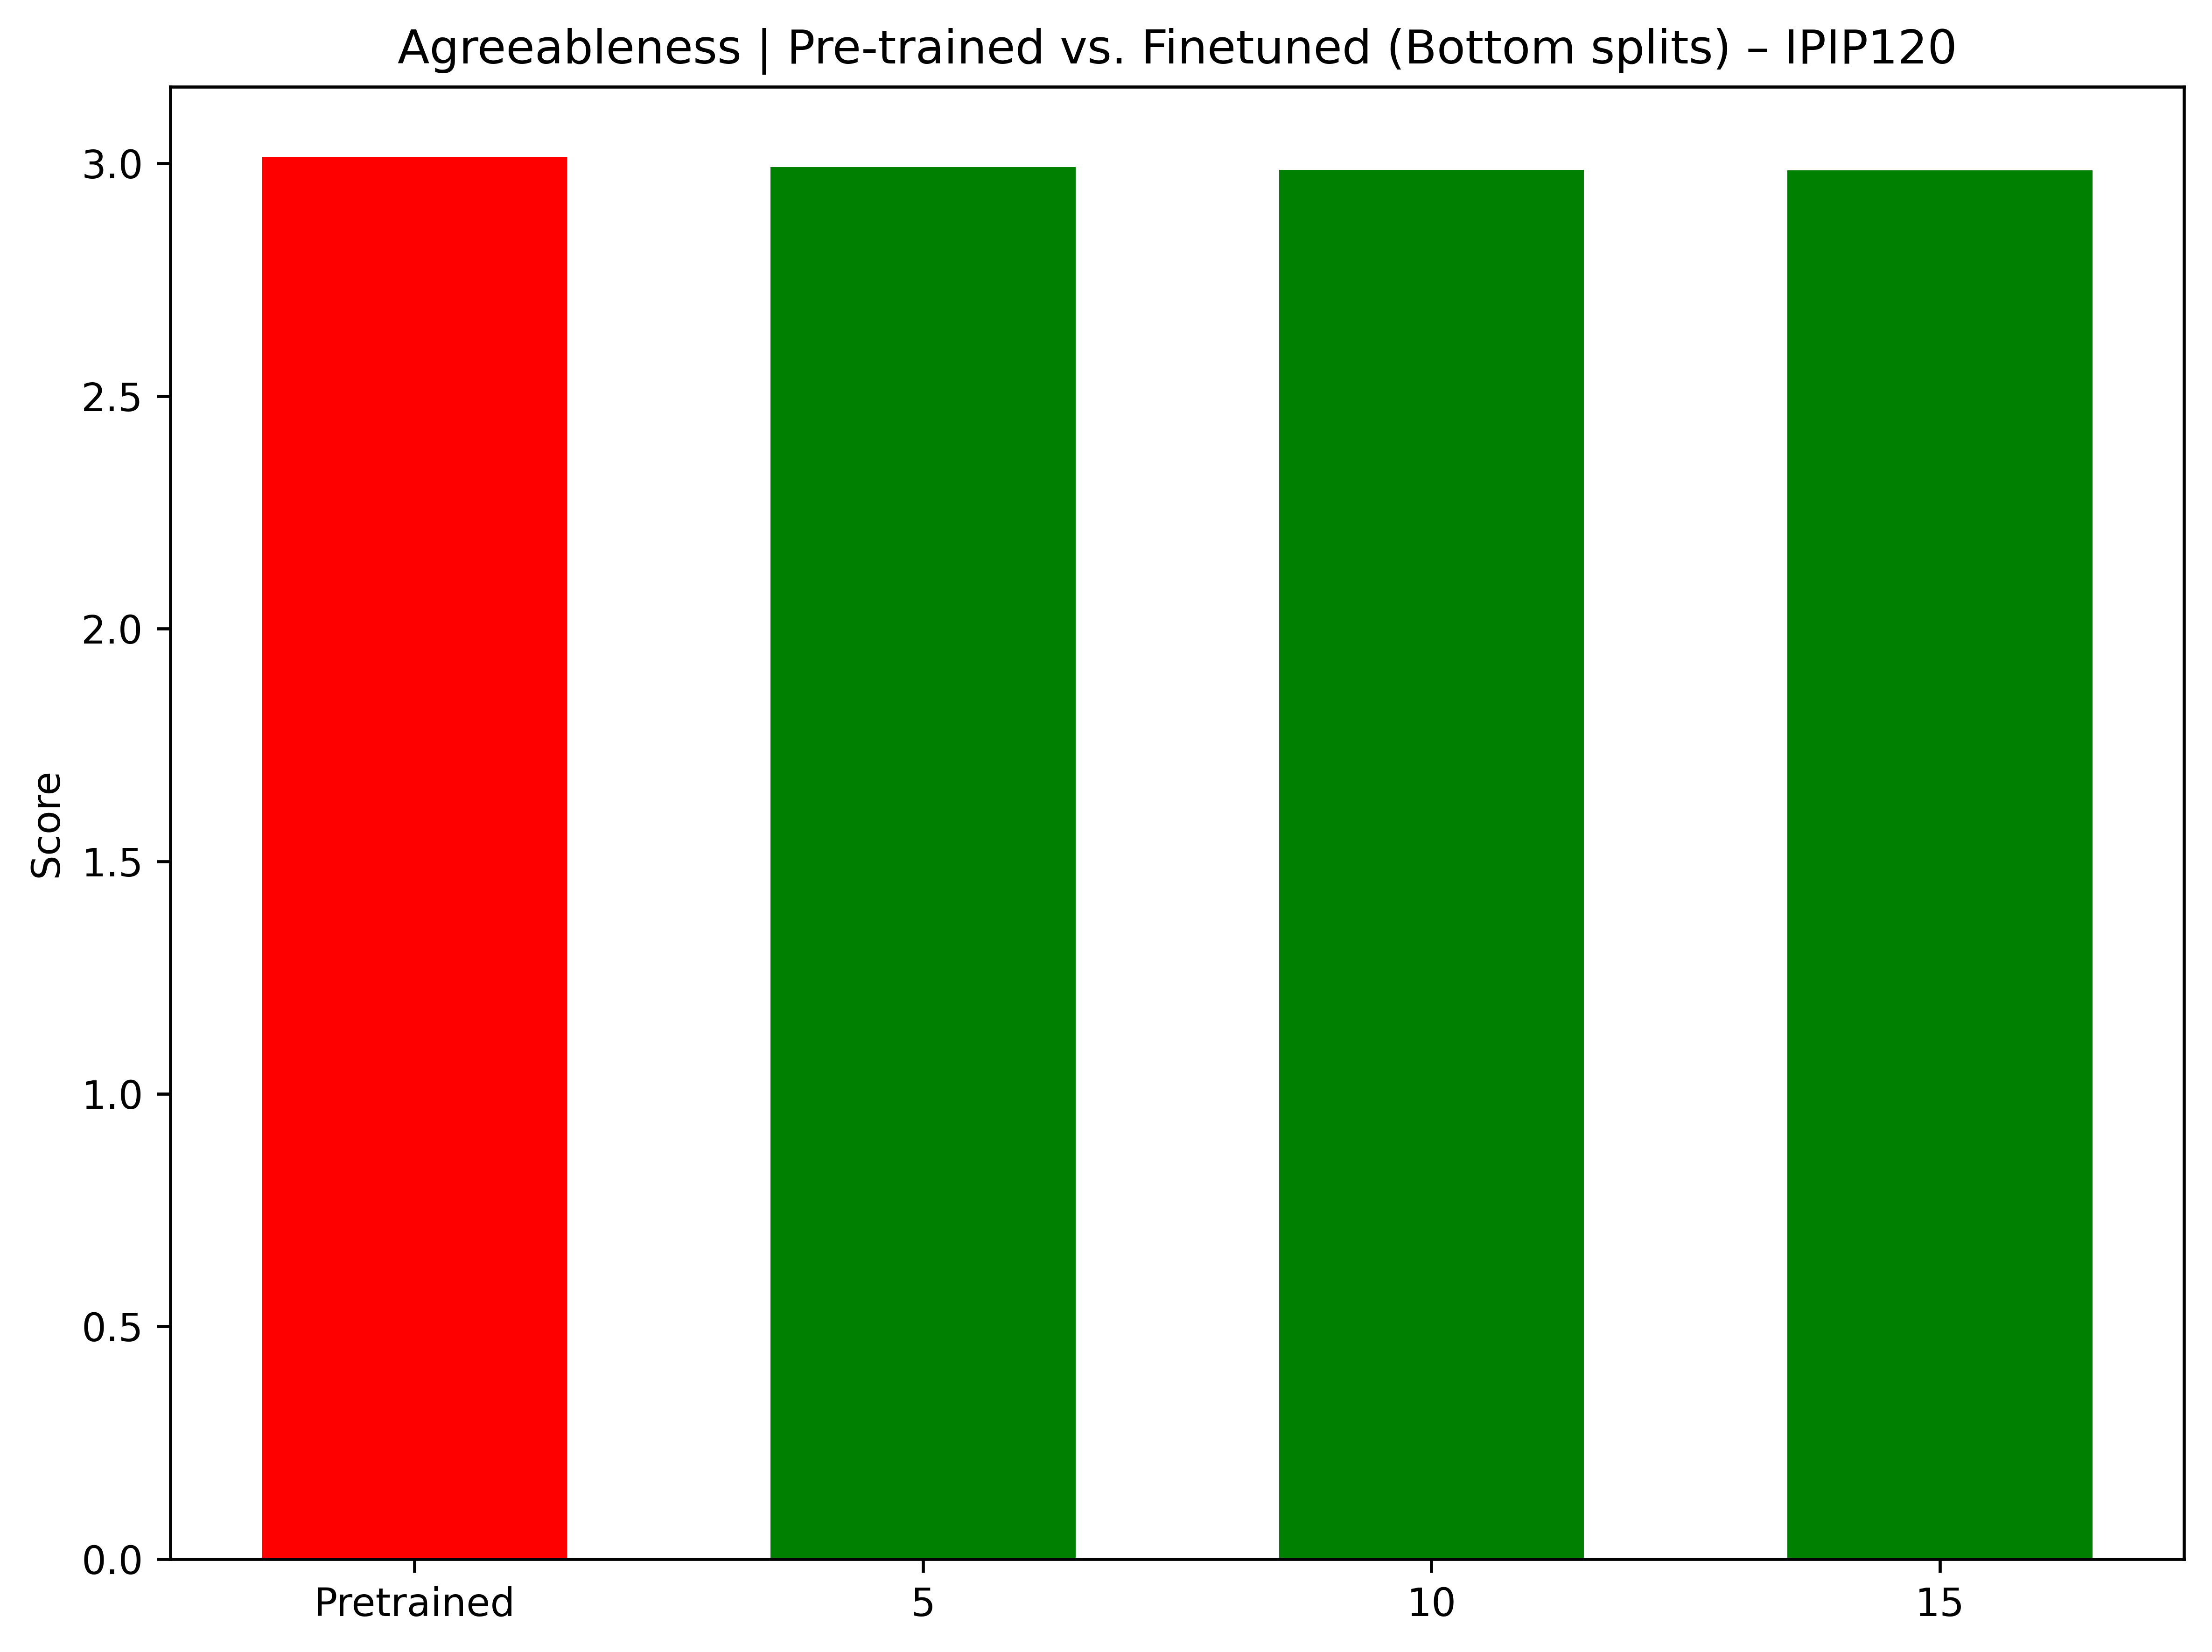
\includegraphics[width=0.8\textwidth]{img/results/w_i_H1_IPIP120_Agreeableness_bottom.png}
    \caption{Agreeableness scores | Pre-trained vs. Finetuned on bottom Pandora splits | IPIP-120}
    \label{fig:w_i_H1_IPIP120_Agreeableness_bottom}
\end{figure}

\subsubsection{LoRA-scale Response Curves}
Models fine-tuned with LoRA on the PANDORA data splits were assessed across a range of LoRA scaling factors from -25 to +25 in order to test Hypothesis H2, which postulated that increasing the LoRA scaling factor would systematically intensify the expression of the targeted trait. The results show the response curves for each OCEAN trait and are shown in figures like Figure \ref{fig:w_i_H2_BFI10_Agreeableness_top} (BFI-10) and Figure \ref{fig:w_i_H2_IPIP120_Conscientiousness_bottom} (IPIP-120).
\\
\begin{figure}[H]
    \centering
    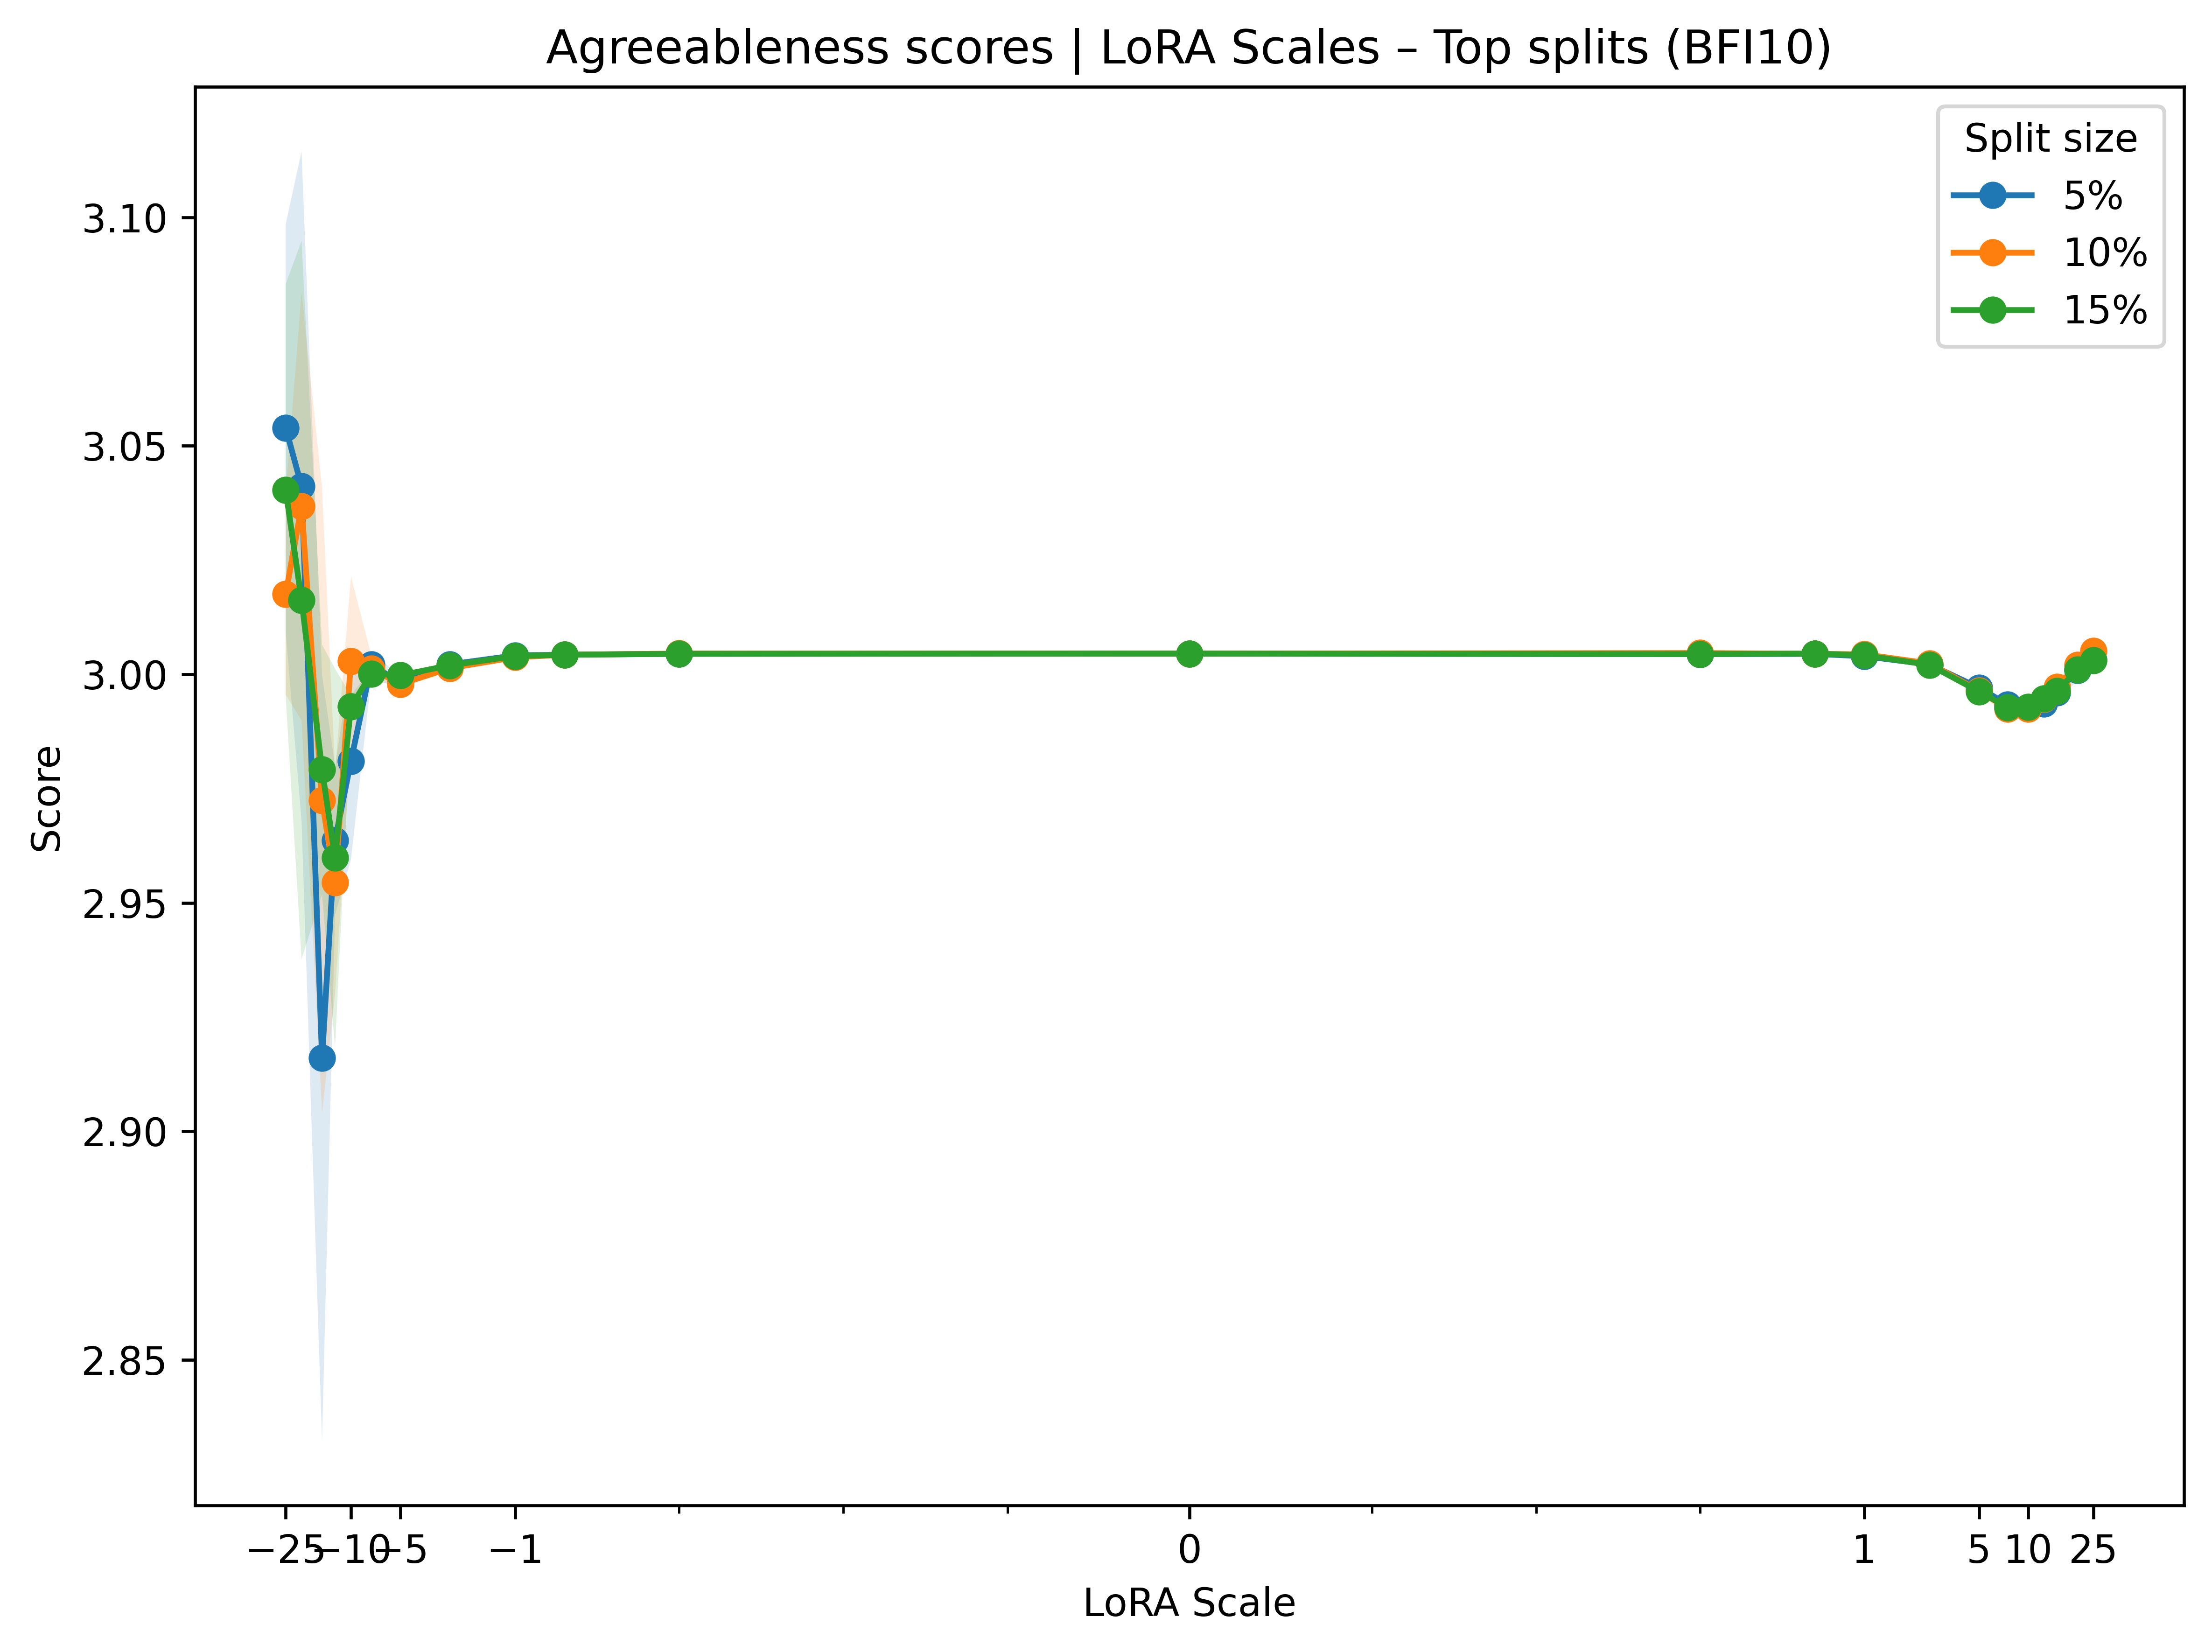
\includegraphics[width=0.8\textwidth]{img/results/w_i_H2_BFI10_Agreeableness_top.png}
    \caption{Agreeableness scores | LoRA Scales - Top splits | BFI-10}
    \label{fig:w_i_H2_BFI10_Agreeableness_top}
\end{figure}

\begin{figure}[H]
    \centering
    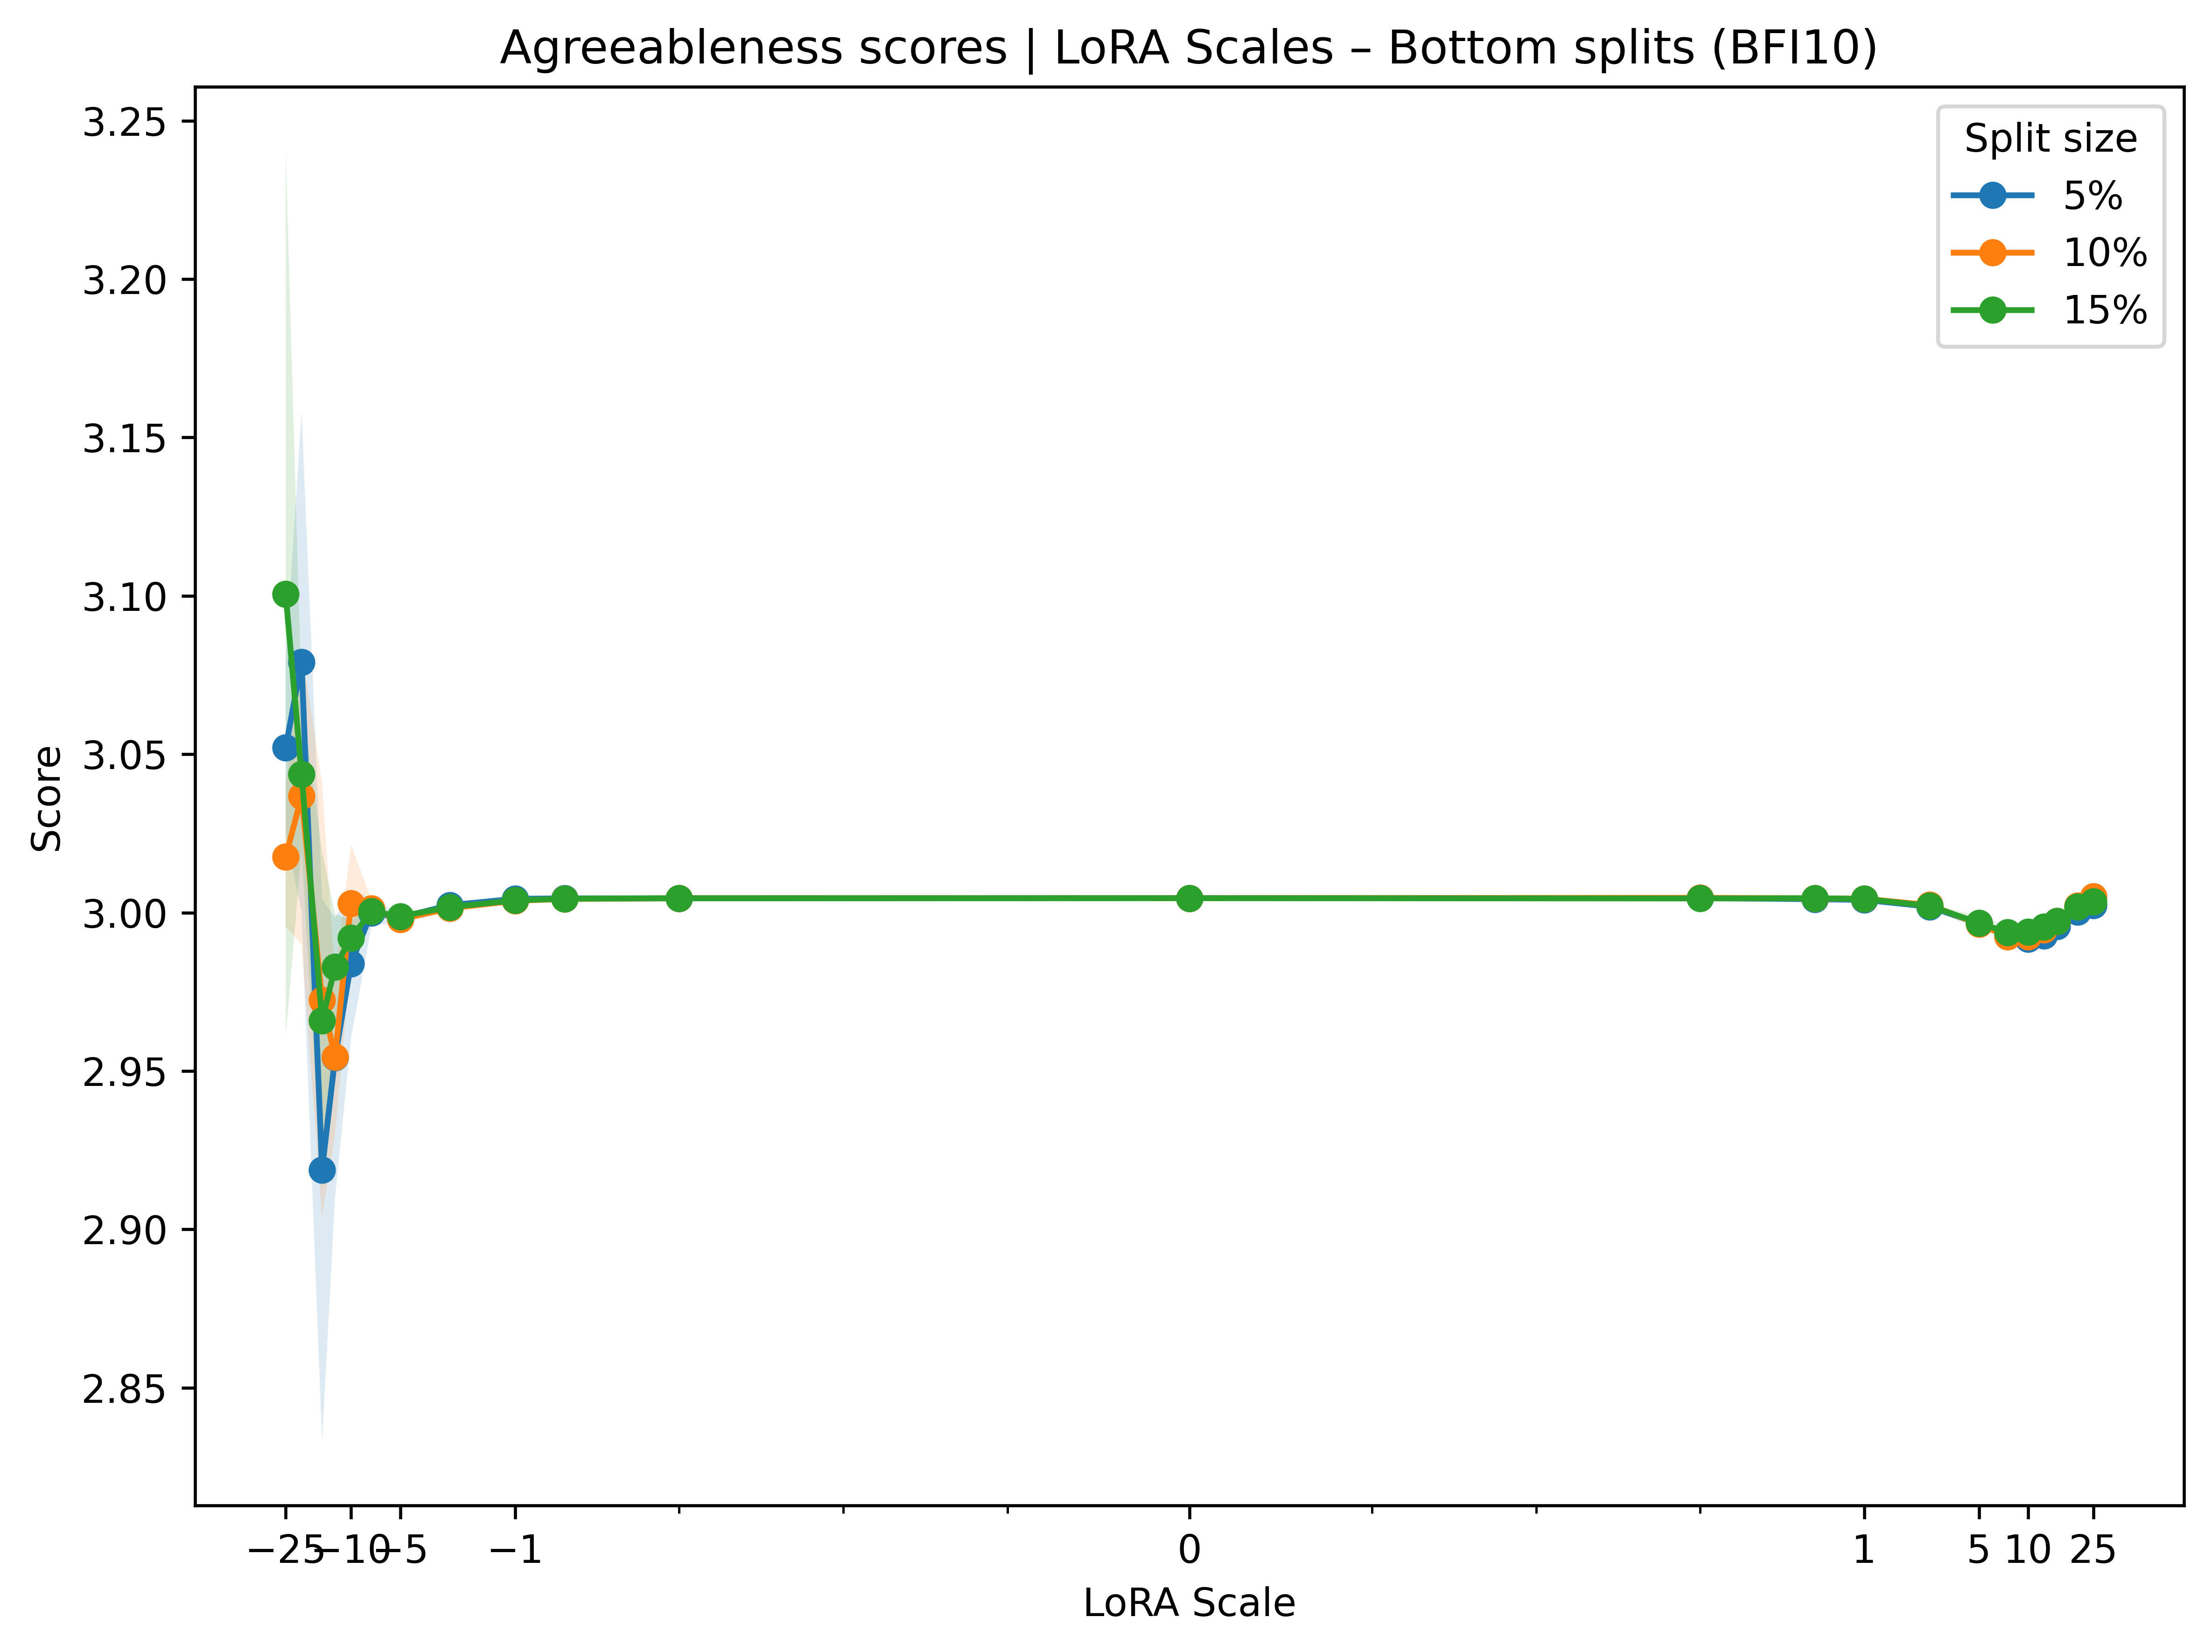
\includegraphics[width=0.8\textwidth]{img/results/w_i_H2_BFI10_Agreeableness_bottom.png}
    \caption{Agreeableness scores | LoRA Scales - Bottom splits | BFI-10}
    \label{fig:w_i_H2_BFI10_Agreeableness_bottom}
\end{figure}

The LoRA scaling factor showed a noticeable, albeit complicated, impact on trait scores for personality traits measured with the BFI-10. Compared to a LoRA scale of 0 (which represents the base LoRA-adapted model without additional scaling), positive LoRA scaling factors typically maintained or slightly amplified the target trait score for models fine-tuned on "top" PANDORA splits (e.g., high Agreeableness, Figure \ref{fig:w_i_H2_BFI10_Agreeableness_top}). However, the target trait score tended to sharply decline, occasionally falling below the score recorded at scale 0, while extreme negative scales (e.g., -10 to -25) tended to cause a plateau or even a slight decrease. Agreeableness scores for the 15\% split (green line) in Figure \ref{fig:w_i_H2_BFI10_Agreeableness_top}, for example, drop considerably towards 2.90 at highly negative scales but stay comparatively stable around 3.00 for positive LoRA scales. When fine-tuned on "top" splits, similar U-shaped or saturating patterns were seen for other traits such as Conscientiousness (Figure \ref{fig:w_i_H2_BFI10_Conscientiousness_top}), Extraversion (Figure \ref{fig:w_i_H2_BFI10_Extraversion_top}), and Openness (Figure \ref{fig:w_i_H2_BFI10_Openness_top}). Positive scaling on a "top" (high Neuroticism) split tended to maintain or slightly increase the Neuroticism score, whereas negative scaling decreased it for the negatively valenced Neuroticism (Figure \ref{fig:w_i_H2_BFI10_Neuroticism_top}). Although the effects were not always perfectly symmetrical or linear, the response curves for models that were fine-tuned on "bottom" splits (e.g., Figure \ref{fig:w_i_H2_BFI10_Agreeableness_bottom}) frequently mirrored these patterns, with positive LoRA scales tending to further suppress the trait and negative scales occasionally leading to an increase. Although there were some differences in the absolute score levels and the magnitude of change at extreme scales, the curve shapes for the various PANDORA split sizes (5\%, 10\%, and 15\%) were generally similar. These results provide partial support for H2, showing that LoRA scaling can influence trait expression, but that the relationship is not always linear and may show saturation or reversal at extreme scaling values. This behavior is consistent with the knowledge that LoRA alters the parameters of the current model within specific bounds \cite{hu_lora_2021, lialin_scaling_2023}.



Similar intricate LoRA scaling dynamics were found in the more thorough IPIP-120 evaluation. Positive LoRA scales typically maintained or marginally raised the target trait score for models adjusted on "top" PANDORA splits (e.g., Figure \ref{fig:w_i_H2_IPIP120_Agreeableness_top}), whereas extreme negative scales frequently caused a noticeable decline. Agreeableness scores for the 15\% split, for instance, show a peak around a LoRA scale of -1 in Figure \ref{fig:w_i_H2_IPIP120_Agreeableness_top}. From there, they gradually decline with increasingly negative scales and stay relatively stable for positive scales. Positive LoRA scales tended to further reduce the target trait score for models fine-tuned on "bottom" splits (e.g., Figure \ref{fig:w_i_H2_IPIP120_Conscientiousness_bottom}), whereas negative scales frequently caused an increase, sometimes dramatically at extreme negative values (e.g., -10 to -25), before possibly declining again. Extreme negative scaling may be pushing the model into an opposing trait space or creating instability, as evidenced by the "rebound" effect at highly negative scales, where the trait score may rise above the scale 0 level. These non-linear responses to LoRA scaling were also seen in the patterns for Neuroticism (Figures \ref{fig:w_i_H2_IPIP120_Neuroticism_top}, \ref{fig:w_i_H2_IPIP120_Neuroticism_bottom}), Extraversion (Figures \ref{fig:w_i_H2_IPIP120_Extraversion_top}, \ref{fig:w_i_H2_IPIP120_Extraversion_bottom}), and Openness (Figures \ref{fig:w_i_H2_IPIP120_Openness_top}, \ref{fig:w_i_H2_IPIP120_Openness_bottom}). Although the precise inflection points and magnitudes varied, the general shape of the curves was consistent across the various PANDORA split sizes (5\%, 10\%, and 15\%). These results show that LoRA can modulate trait intensity, which further supports H2. However, they also show non-linear and sometimes counterintuitive effects at extreme scaling factors, which may be due to the complex interaction between the learned representations of the base model and the LoRA adapter \cite{zhao_lora_2024, biderman_lora_2024}.

\subsection{Emotion-related Experiments}
Experiments were carried out to determine whether adjusting GPT-2 on the TweetEval-Emotion data splits (Anger, Joy, Optimism, and Sadness) would result in changes to its PANAS-X emotion scores in accordance with H1. The findings are displayed in figures like Figure \ref{fig:w_i_H1_Emotion_anger} (fine-tuned on Anger) and Figure \ref{fig:w_i_H1_Emotion_joy} (fine-tuned on Joy), which use weighted Likert scoring and prompts with response options. The model's assessed Anger score (Figure \ref{fig:w_i_H1_Emotion_anger}, first green bar) rose from a pre-trained level of roughly 1.25 to roughly 1.65 after it was adjusted on the "Anger" split. It's interesting to note that while optimism stayed mostly unchanged, adjusting anger also caused sadness and joy to slightly increase (from ~1.25 to ~1.60 and ~1.25, respectively). This implies that the model learns a more broadly elevated emotional responsiveness, or that the linguistic expressions of anger in the training data may share characteristics with those of sadness and joy.
\\
After fine-tuning on the "Joy" split (Figure \ref{fig:w_i_H1_Emotion_joy}), the Joy score rose from a pre-trained level of about 1.30 to about 1.80. The evaluated Anger (~1.65 from ~1.30), Sadness (~1.75 from ~1.30), and Optimism (~1.70 from ~1.30) scores all rose when Joy was fine-tuned. Fine-tuning on "Optimism" (Figure \ref{fig:w_i_H1_Emotion_optimism}) and "Sadness" (Figure \ref{fig:w_i_H1_Emotion_sadness}) revealed a similar pattern of the target emotion rising in tandem with increases in other emotions. Since fine-tuning on particular emotion data does increase the target emotion, these results are consistent with H1. The co-amplification of other emotions, however, raises the possibility that either the model is not learning very different emotional expressions or that the PANAS-X items for various emotions capture overlapping linguistic cues in the model's output. This is consistent with studies that demonstrate that while LLMs are capable of modeling emotions, they might not fully understand their subtleties or clear boundaries like humans do \cite{chang_modeling_2024, liu_emollms_2024}.
\\
Models LoRA optimized on the TweetEval-Emotion splits were assessed across the LoRA scaling factors in order to examine H2 in relation to emotions. The LoRA scale was plotted against the Anger, Sadness, Joy, and Optimism PANAS-X scores. When the LoRA scale was increased, the assessed Anger score (blue line) increased dramatically from about 1.0 at scale 0 to over 2.75 at scale +25 for a model that was fine-tuned on the "Anger" split (Figure \ref{fig:w_i_H2_Emotion_anger}). Though not as much as anger, the scores for sadness, joy, and optimism also rose with positive scaling. In general, all emotion scores were suppressed by negative LoRA scaling.
The model that was adjusted for "Joy" showed a similar pattern (Figure \ref{fig:w_i_H2_Emotion_joy}). With positive LoRA scaling, the Joy score (green line) increased sharply, rising from roughly 1.0 at scale 0 to almost 2.4 at scale +25. With positive scaling, the scores for anger, sadness, and optimism also showed an upward trend. Similar behaviors were shown by the models that were fine-tuned on "Optimism" (Figure \ref{fig:w_i_H2_Emotion_optimism}) and "Sadness" (Figure \ref{fig:w_i_H2_Emotion_sadness}). The target emotion score responded most strongly to positive LoRA scaling, and other emotion scores also tended to rise, albeit frequently less sharply. These findings provide strong support for H2 for emotions, showing that the target emotional expression's intensity can be efficiently controlled by the LoRA scaling factor. It is possible that the LoRA adaptation is learning a general "emotionality" vector that, when scaled, amplifies multiple affective dimensions with a stronger effect on the specifically trained emotion, as evidenced by the concurrent increase in other emotion scores. This might be a reflection of how emotional language is interconnected or how the model represents emotional states \cite{mozikov_good_2024, zhao_both_2024}.

\subsection{Task Arithmetic Experiments}
In order to test H3, the task arithmetic experiments loaded a GPT-2 model that had been fully fine-tuned on a particular PANDORA personality split (for example, "agreeableness-top-5\%) and then applied LoRA adapters that had been separately trained on one of the TweetEval-Emotion splits (for example, "anger"). The combined model's OCEAN personality scores were then evaluated using the emotion adapter's range of LoRA scaling factors.
When a base model optimized for high Agreeableness is combined with LoRA adapters for Anger, the BFI-10 OCEAN scores are displayed in Figure \ref{fig:w_i_h3.1_BFI10_agreeableness-top-5_anger}. There is a general trend for the Agreeableness score (red line) to slightly decline as the LoRA scale for anger rises from negative to positive values, especially at higher positive LoRA scales (e.g., from ~3.00 at scale 0 to ~2.95 at scale +25). Positive Anger LoRA scaling tends to increase neuroticism (purple line) (from ~2.98 to ~3.03). Openness (blue line) stays largely constant, but extraversion (green line) and conscientiousness (orange line) exhibit less frequent or noticeable shifts. According to psychological understanding of how anger may manifest in relation to these traits, this suggests that superimposing a "anger" adaptation can indeed modulate the base personality profile, possibly by increasing neuroticism and decreasing agreeableness \cite{oshio_resilience_2018}.
\\
The Agreeableness score tends to stay constant or slightly increase with positive LoRA scaling when the same high-Agreeableness base model is combined with LoRA adapters for Joy (Figure \ref{fig:w_i_h3.1_BFI10_agreeableness-top-5_joy}). Positive Joy scaling results in a slight decrease in neuroticism. Analyses of the combinations with Sadness (Figure \ref{fig:w_i_h3.1_BFI10_agreeableness-top-5_sadness}) and Optimism (Figure \ref{fig:w_i_h3.1_BFI10_agreeableness-top-5_optimism}) revealed different modulations of the base OCEAN profile. For instance, on positive scales, Sadness LoRA adapters tended to increase neuroticism while decreasing agreeableness and extraversion. These results provide support for H3, showing that the model's personality profile can be altered in ways that are generally consistent with the nature of the combined traits and emotions by using an arithmetic-like composition of trait/emotion vectors (through the addition of a LoRA adapter). These more subtle behavioral traits seem to be covered by the task arithmetic principle, which has been shown to apply to task-specific skills \cite{ilharco_editing_2023, chronopoulou_language_2023}.
\\
\begin{figure}[H]
    \centering
    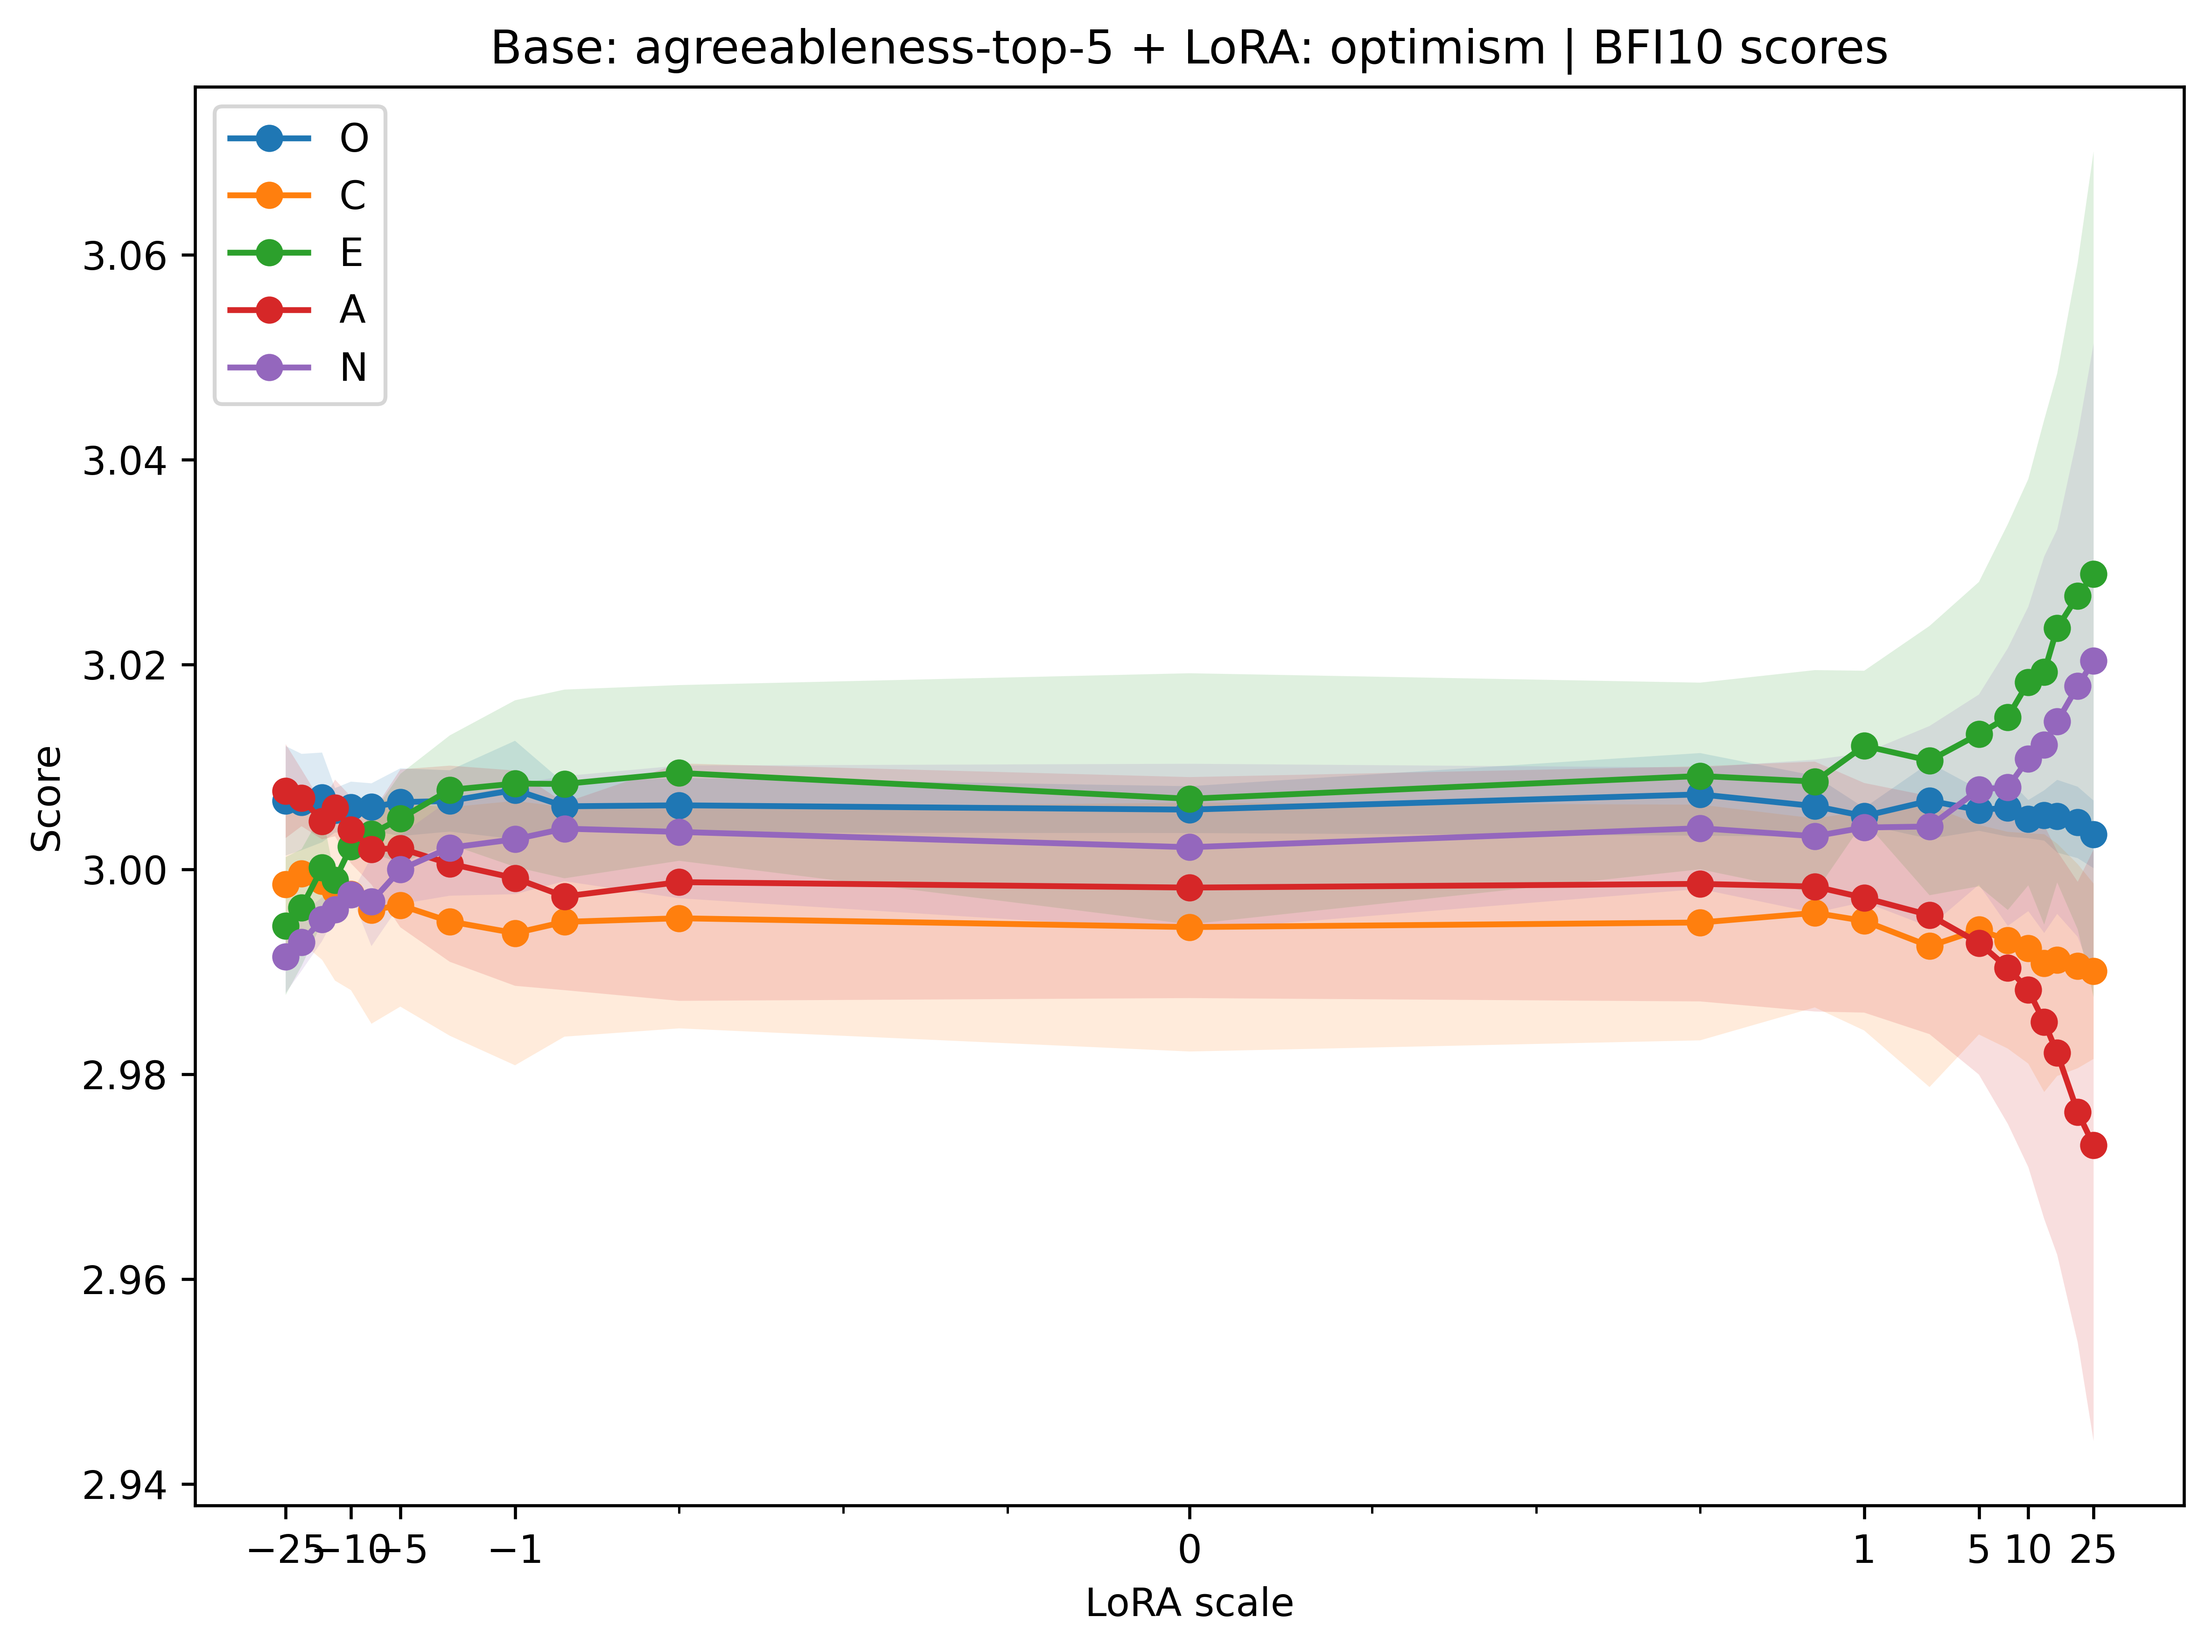
\includegraphics[width=0.8\textwidth]{img/results/w_i_h3.1_BFI10_agreeableness_optimism.png}
    \caption{Agreeableness-top-5 + LoRA optimism | BFI-10 scores}
    \label{fig:w_i_h3.1_BFI10_agreeableness-top-5_optimism}
\end{figure}

In an additional set of tests, LoRA adapters trained on PANDORA personality splits were paired with base models that had been completely optimized on particular TweetEval-Emotion splits. Figure \ref{fig:w_i_h3.1_PANASX_anger_agreeableness-top-5}, for example, displays the PANAS-X emotion scores when a base model optimized for Anger is coupled with LoRA adapters for high Agreeableness. The measured anger score (blue line) clearly and significantly decreases as the LoRA scale for agreeableness rises positively (from ~2.25 at scale 0 to ~1.0 at scale +25). While joy (green line) and optimism (red line) either slightly increase or stay the same, sadness (orange line) likewise declines. This implies that in an anger-specialized model, using a high-Agreeableness adaptation can successfully reduce the expression of negative emotions like sadness and anger.
\\
The effect on Anger is less noticeable, but still a slight decrease at positive scales, when the Anger base model is combined with LoRA for high Conscientiousness (Figure \ref{fig:w_i_h3.1_PANASX_anger_conscientiousness-top-5}). Anger and sadness are moderately reduced when combined with high Extraversion LoRA (Figure \ref{fig:w_i_h3.1_PANASX_anger_extraversion-top-5}), while joy and optimism are slightly increased. While high Openness LoRA (Figure \ref{fig:w_i_h3.1_PANASX_anger_openness-top-5}) has a less obvious effect, it may marginally increase positive emotions at higher scales. In contrast, high Neuroticism LoRA (Figure \ref{fig:w_i_h3.1_PANASX_anger_neuroticism-top-5}) tends to maintain or slightly increase Anger and Sadness scores. These findings support H3 even more by showing that personality-specific LoRA adapters can alter an emotion-fine-tuned base model's emotional expression profile. Human psychological knowledge of these constructs is intuitively consistent with the observed interactions, such as high agreeableness lowering anger \cite{feng_five-factor_2024, david_watson_panas-x_1994}.
\\
A more subtle aspect of task arithmetic is examined by the H3.2 plots (e.g., Figure \ref{fig:w_i_h3.2_BFI10_agreeableness-bottom_anger_agreeableness}), which examine how the size of the PANDORA data split used to train the base personality model affects the result when combined with an emotion-LoRA adapter. These plots monitor a single target personality trait of the combined model, such as agreeableness. For instance, the Agreeableness score is observed when LoRA adapters for "anger" are combined with a base model that has been fine-tuned on "agreeableness-bottom" (using 5\%, 10\%, or 15\% PANDORA splits). The plots typically demonstrate the significant influence of the emotion adapter's LoRA scaling, frequently producing a V- or U-shaped curve for the target personality trait. Although the various lines (which represent the 5\%, 10\%, or 15\% base model training split) frequently exhibit comparable patterns, they may vary in terms of the precise score levels or the strength of the LoRA scaling effect. In Figure \ref{fig:w_i_h3.2_BFI10_agreeableness-bottom_anger_agreeableness}, for example, adding "anger" LoRA at positive scales tends to further reduce the base model's already low Agreeableness, whereas adding "anger" LoRA at extreme negative scales can paradoxically increase Agreeableness. Instead of radically altering the form of the response to the emotion LoRA, the size of the base model's PANDORA split seems to control the strength of these effects. Other combinations, like a "conscientiousness-top" base model with different emotion LoRAs, show similar complex interactions (e.g., Figure \ref{fig:w_i_h3.2_BFI10_conscientiousness-top_joy_conscientiousness}). According to these findings, task arithmetic works well, but there are non-trivial interactions between the superimposed LoRA adaptation and the base model's properties, including the data it was trained on.

\subsection{Robustness Analyses}

\subsubsection{Different Splits \& Questionnaires}
The BFI-10 and the IPIP-120 are two distinct personality inventories that are used to evaluate the consistency of personality measures. In general, the IPIP-120 results mirrored the directional effects of LoRA scaling (H2) and fine-tuning (H1) seen with the BFI-10, though the precise magnitudes and curve shapes occasionally varied. For instance, if improving on a "high Extraversion" PANDORA split resulted in a higher Extraversion score on the BFI-10, the IPIP-120 Extraversion scale usually showed a comparable increase (see, for instance, Figure \ref{fig:w_i_H1_BFI10_Extraversion_top} with Figure \ref{fig:w_i_H1_IPIP120_Extraversion_top}). The observed personality shifts are given more credibility by this consistency across instruments, despite the fact that their item content and length vary, indicating that they are more than just the result of a single questionnaire. This supports research showing that, when properly designed, various FFM instruments tend to capture comparable underlying constructs \cite{maples_test_2014, johnson_measuring_2014}.
\\
PANDORA data splits representing the top/bottom 5\%, 10\%, and 15\% of authors for each OCEAN trait were fine-tuned for the experiments for H1 and H2. The size of the PANDORA split (5\%, 10\%, or 15\%) did not seem to have a significant impact on the final assessed personality scores for full fine-tuning (H1); the green bars in the H1 plots are typically of similar height for a given trait and condition (e.g., Figure \ref{fig:w_i_H1_BFI10_Agreeableness_top}). The response curves for the 5\%, 10\%, and 15\% splits generally followed similar overall patterns for LoRA fine-tuning and subsequent scaling (H2), although there were frequently variations in the absolute score levels or the sensitivity to extreme LoRA scaling factors (e.g., the shaded areas or the spread of the lines in Figures \ref{fig:w_i_H2_BFI10_Agreeableness_top} or \ref{fig:w_i_H2_IPIP120_Conscientiousness_bottom}). This implies that the amount of data used for the initial LoRA fine-tuning can alter the baseline trait expression and its responsiveness to scaling, even though the core effect of LoRA scaling remains constant. Although the visual results shown are before this debiasing, the debiasing step applied to PANDORA OCEAN scores, taking into account inter-trait correlations (Figure \ref{fig:ocean_trait_correlation_pandora}) and the mean profiles of the splits (Figure \ref{fig:pandora_splits_ocean_heatmap}), was meant to more clearly isolate the impact of the target trait.

\subsubsection{Prompt Sensitivity Analyses}
To assess sensitivity to minor variations in the evaluation prompting protocol, experiments were conducted by either including the explicit Likert scale response options (e.g., "Disagree strongly", "Disagree a little", etc.) in the prompt or excluding them. The "include options" variant with "weighted" scoring (w\_i\_... plots) is the basis for the results shown in the main findings sections (6.1, 6.2, 6.3). The general patterns and directional effects of fine-tuning and LoRA scaling are substantially the same for both prompting conditions when compared to the "exclude options" variant (w\_e\_... plots). Figure \ref{fig:w_i_H1_BFI10_Agreeableness_top} (include options) and Figure \ref{fig:w_e_H1_BFI10_Agreeableness_top} (exclude options), for instance, display comparable patterns of Agreeableness scores for pre-trained versus fine-tuned models. Similarly, whether or not options are explicitly listed does not affect the characteristic shapes of the LoRA scaling response curves, such as those for BFI-10 Agreeableness (see Figure \ref{fig:w_i_H2_BFI10_Agreeableness_top} versus Figure \ref{fig:w_e_H2_BFI10_Agreeableness_top}). This implies that the GPT-2 model's unique Likert-scale scoring pipeline, which assesses the model's probability of producing each anchor text, is comparatively resistant to this particular prompt variation. This is in contrast to some research that found that using direct self-assessment with multiple-choice questions (MCQs) increased sensitivity to prompt format \cite{gupta_self-assessment_2024, shu_you_2024}. Some of these sensitivities may be lessened by the current approach, which assesses the likelihoods of each option rather than asking the model to select one.
\\
Two Likert score types were extracted by the evaluation pipeline: "weighted" (a continuous score based on the probability distribution across all options) and "max" (the single Likert option with the highest probability). "Weighted" scores are used to report the key findings. In general, the directional effects and general patterns are comparable when comparing these with "max" scores (e.g., m\_i\_... plots vs. w\_i\_... plots). The BFI-10 Agreeableness H1 bar charts, for example (see Figure \ref{fig:w_i_H1_BFI10_Agreeableness_top} and Figure \ref{fig:m_i_H1_BFI10_Agreeableness_top}) demonstrate similar correlations between pre-trained and fine-tuned scores. Similar shapes can also be seen in the LoRA scaling curves (see Figure \ref{fig:w_i_H2_BFI10_Agreeableness_top} and Figure \ref{fig:m_i_H2_BFI10_Agreeableness_top}). In contrast to the discrete "max" scores, the continuous "weighted" scores typically yield smoother curves and might capture more subtle changes in the model's preferences. The observed effects are made more robust by the overall consistency of these scoring techniques. The distribution of selected Likert options using the "max" method is displayed in the Likert option frequency vs. inventories | Method = max\_prob plots (Figure \ref{fig:likert_option_frequency_vs_inventories_method_max_prob}), whereas the density of the continuous weighted scores is displayed in the Likert option frequency vs. inventories | Method = weighted\_prob plots (Figure \ref{fig:likert_option_frequency_vs_inventories_method_weighted_prob}). Both show that the weighted scores frequently form multi-modal distributions, indicating complex internal preferences, and that the model does not pick options uniformly.

\subsubsection{Distributional Effects Across Trait Percentiles}
Authors with extreme trait expressions (top/bottom k\%) can be used to create fine-tuning splits using the author-level OCEAN scores provided by the PANDORA dataset. The mean OCEAN profiles of authors within each of these balanced data splits are visualized in the heatmap shown in Figure \ref{fig:pandora_splits_ocean_heatmap}. This "ground truth" demonstrates that although authors with a split like "Openness-top-5\%" do, on average, have very high Openness scores, they also have particular profiles on other OCEAN traits (e.g., moderately high Extraversion, average Conscientiousness). One important factor is the natural co-occurrence of traits in the training data. The goal of the fine-tuning procedure (H1) is to change the model's evaluated score on the desired characteristic (for example, Openness for the "Openness-top-5\%" split). In order to isolate the effect of the primary trait that the fine-tuning split is targeting, the debiasing step outlined in the methodology (Section 5.4.4) is intended to statistically account for these co-occurring traits in the input data when interpreting the model's output scores. Beyond the visual examination of raw score plots, a thorough results analysis would be necessary to determine whether this debiasing was successful in exposing more distinct trait-specific changes.
\\
The distribution of the LLM's responses across the Likert scale options for the PANAS-X, BFI-10, and IPIP-120 inventories, aggregated across all experimental conditions, is depicted in the plots in Figure \ref{fig:likert_option_frequency_vs_inventories_method_max_prob} (for "max" scoring) and Figure \ref{fig:likert_option_frequency_vs_inventories_method_weighted_prob} (for "weighted" scoring). It is clear that option 3 ("Neither agree nor disagree" or equivalent neutral midpoint) is commonly selected for the "max" scoring in all inventories, especially for BFI-10 and IPIP-120. Less often, the extreme ends, options 1 and 5, are selected. This implies that if the underlying preference shift is not sufficiently strong to make an extreme option the single most likely option, the model may have a tendency to skew toward neutral responses when applying the "max" probability criterion. This could reduce the observed effects of fine-tuning or scaling. The continuous and frequently multi-modal "weighted" score distributions (Figure \ref{fig:likert_option_frequency_vs_inventories_method_weighted_prob}) show that the model gives several response options non-negligible probabilities. Because weighted scoring takes into account data from the full probability distribution rather than just the mode, it is a useful tool for capturing these subtle preferences. With fine-tuning or LoRA scaling, the distributions' shapes (such as skewness and modality) may systematically change, reflecting changes in the model's underlying response tendencies that go beyond simple mean score changes.

\subsection{Summary Of Key Empirical Findings}
Several important conclusions about the evaluation and modification of personality and emotion traits in the GPT-2 language model were drawn from the empirical research done for this thesis.
\\
First, with regard to Hypothesis H1, complete fine-tuning on TweetEval-Emotion data splits and PANDORA personality data splits typically led to quantifiable changes in the model's evaluated OCEAN and PANAS-X scores, respectively. Although the size of these changes was frequently small, these shifts were generally in the predicted direction (for example, fine-tuning on high-Agreeableness data led to higher assessed Agreeableness). The target emotion increased when emotion-specific data was fine-tuned, but other emotions were often co-amplified as well, indicating overlapping linguistic cues or a learned general emotional responsivity.
\\
Second, addressing Hypothesis H2, models fine-tuned with LoRA showed a clear, albeit complex and non-linear, ability to modulate the intensity of expressed emotion and personality traits when different LoRA scaling factors were applied. In contrast to negative scaling, which either suppressed the target trait or emotion or, in certain situations at extremely negative values, produced a rebound effect, positive LoRA scaling typically increased the target trait or emotion. Although its effects are not always directly proportional and may show saturation, this demonstrates that LoRA scaling can function as a control mechanism.
Third, the task arithmetic experiments (Hypothesis H3) demonstrated that such compositions can indeed change the overall personality and emotional profile of the model. These experiments combined a fully optimized base model with LoRA adapters trained on a different trait/emotion. These changes generally followed the pattern of the combined traits and emotions (for example, adding "high Agreeableness" LoRA to a "Anger" base model tended to reduce assessed anger). This lends credence to the notion that learned behavioral traits can be somewhat arithmetically combined.
\\
Lastly, robustness analyses showed that, when employing the custom likelihood-based scoring pipeline, the observed effects were comparatively robust to slight changes in the evaluation prompting protocol (inclusion/exclusion of Likert options) and were generally consistent across various personality inventories (BFI-10 and IPIP-120). Similar directional results were also obtained by selecting the Likert scoring method (weighted average vs. maximum probability), with weighted scores providing more continuous, nuanced measurements. In order to better isolate particular trait effects in subsequent analyses, a debiasing technique was suggested, acknowledging the inherent co-occurrence of traits in the PANDORA training data.


%%%%%%%%%%%%%%%%%%%%% Chapter 7 %%%%%%%%%%%%%%%%%%%%%%
\chapter{Discussion}
\thispagestyle{empty}

\subsection{Interpretation Of Findings}
\subsubsection{Confirmation of LLM Malleability to Trait-Specific Data}
The general principle that LLMs learn to mimic patterns present in their training data is confirmed by the findings pertaining to H1, where complete fine-tuning on personality and emotion-specific data splits resulted in corresponding shifts in assessed traits \cite{jiang_evaluating_2023, pan_llms_2023, safdari_personality_2023}. Though sometimes with small effect sizes, the GPT-2 model was able to incorporate unique linguistic signals from the PANDORA dataset, which included author-level personality scores, and the TweetEval-Emotion dataset, which included emotion labels. It's particularly intriguing to note that improving scores for one emotion (like joy) also raised scores for other emotions (like anger and sadness). This could suggest that the model learns a more generalized "emotional intensity" or "expressiveness" instead of highly differentiated emotional states, or that the linguistic markers for these emotions in the training data are not completely distinct. This is consistent with the complexity of human emotion, where different emotions may share expressive or physiological elements \cite{paul_towards_2020, nummenmaa_bodily_2014}, and computational results that suggest LLMs may have trouble recognizing the subtle differences between discrete emotions without highly specialized training or architectural changes \cite{chang_modeling_2024, liu_emollms_2024}.

\subsubsection{LoRA Scaling as a Nuanced Control Mechanism}
The findings for H2 show that LoRA scaling factors provide a practical, albeit non-linear, way to regulate the degree of expressed emotion and personality traits. One potent feature of PEFT methods is the ability to change the level of trait expression by varying a single scaling parameter \cite{hu_lora_2021}. The observed saturation effects or even reversals at extreme scaling values (such as very large positive or negative scales) imply that the LoRA adaptation works within the constraints of the low-rank update learned and the representational space of the base model. Excessive scaling could cause instability or activate unintended correlated features, as well as out-of-distribution behavior for the adapter's influence. This subtle control is in line with LoRA's method of adding a low-rank perturbation to frozen weights; the magnitude of this perturbation is directly modulated by the scaling factor \cite{biderman_lora_2024, zhao_lora_2024}. Extreme scaling in either direction may disrupt the coherent expression of a trait, possibly by moving the model into an unfamiliar part of its activation space or by overemphasizing certain aspects at the expense of others, as suggested by the U-shaped curves that are occasionally seen, especially for personality traits.

\subsubsection{Task Arithmetic for Composing Behavioral Traits}
Behavioral traits acquired through fine-tuning can be composed or modified by combining models or their adapters, as demonstrated by the task arithmetic experiments (H3). The resulting personality profile changed in ways that were frequently intuitively consistent with the psychological interaction of those constructs when LoRA adapters trained for a particular emotion were added to a base model that had been fine-tuned for a particular personality trait (e.g., Agreeableness LoRA reducing expressed Anger). As suggested by previous work on task arithmetic for more explicit tasks \cite{ilharco_editing_2023, chronopoulou_language_2023}, this supports the notion that learned representations for various behavioral characteristics might occupy somewhat distinct or directionally identifiable regions in the model's weight space, allowing for meaningful arithmetic combinations. The interpretability and controllability provided by this combined approach are further highlighted by the fact that these effects were detectable by varying the LoRA scaling factor of the "added" trait. The intricacy seen in the H3.2 plots, where the interaction was impacted by the size of the base model's training data, implies that the "strength" or "clarity" of the learned trait of the base model also affects how it interacts with superimposed adaptations.

\subsubsection{Robustness of Assessment and Implications of Scoring Choices}
The general findings are supported by the robustness analyses. The observed effects appear to be independent of a single instrument, as evidenced by the consistency between personality assessments on the BFI-10 and IPIP-120. The custom likelihood-based scoring pipeline's relative insensitivity to the explicit inclusion/exclusion of Likert options in the prompt is a good thing because it shows that it is somewhat resilient to small prompt variations, which is a known problem in LLM evaluation \cite{gupta_self-assessment_2024, shu_you_2024}. Although weighted probability scoring provides a more continuous and potentially sensitive measure, the similarity in directional findings between "max" and "weighted" probability scoring indicates that both capture the underlying preference shifts. The importance of the scoring method is highlighted by the distributional plots of Likert responses (Figures \ref{fig:likert_option_frequency_vs_inventories_method_max_prob} and \ref{fig:likert_option_frequency_vs_inventories_method_weighted_prob}), which show a tendency towards neutral responses (option 3) with "max" scoring and more dispersed, multi-modal distributions with "weighted" scoring. The probabilistic nature of LLM outputs seems to be better captured by the "weighted" approach, which also prevents information loss from merely taking the argmax.

\subsection{Comparison With Prior Work}
\subsubsection{Alignment with Existing Computational Literature}
The results of this thesis support and expand on a number of themes in the growing body of research on emotion and personality in LLMs. Numerous studies have found that LLMs can display quantifiable personality-like traits when evaluated using human psychometric tools \cite{caron_manipulating_2023,safdari_personality_2023,sorokovikova_llms_2024,jiang_personallm_2024}. Similar to this, researchers like Liu et al. (2024) and Chang (2024) have shown that LLMs can produce text that expresses particular emotions or sentiments, and that these can be influenced by training or prompting. By methodically applying these assessment paradigms following focused fine-tuning on data chosen for extreme trait/emotion expression, this thesis makes a contribution.

\subsubsection{Controllability via Fine-tuning and Prompting}
The effective, if occasionally modest, induction of target personality and emotion traits through full fine-tuning (H1) is consistent with research by Pan \& Zeng (2023) and Jiang et al. (2023), which demonstrated that training data can influence LLM personality. Though accomplished here through PEFT parameter scaling, the efficacy of LoRA scaling (H2) in modulating trait intensity provides a more granular control mechanism than simple fine-tuning, similar to the dynamic personality customization investigated through activation engineering by Allbert et al. (2025) or the intensity-level shaping via linguistic qualifiers by Safdari et al. (2023). Without highly specialized training or architectures, LLMs may learn broader affective patterns rather than highly discrete states, as evidenced by the co-amplification of multiple emotions seen during emotion fine-tuning \cite{chang_modeling_2024}.

\subsubsection{Task Arithmetic for Behavioral Traits}
The concepts presented by Ilharco et al. (2023) and Chronopoulou et al. (2023) are extended from task-specific skills to the more complex areas of personality and emotion in the task arithmetic experiments (H3). This thesis shows that a similar compositional logic can be applied to behavioral traits, whereas their work concentrated on combining task vectors from PEFT modules or full models for functional tasks (such as translation or QA). Even for these intricate psychological constructs, the idea of modular, somewhat linearly combinable learned representations is supported by the ability to "add" an emotional LoRA adapter to a personality-fine-tuned model and see predictable changes in its overall profile.

\subsubsection{Robustness and Methodological Considerations}
This thesis is relevant to the issues raised by Gupta et al. (2024), Shu et al. (2024), and Sühr et al. (2023) regarding the validity and reliability of applying human psychometric tests to LLMs. The sensitivity of LLMs to prompt format and option order, as well as their inability to replicate human factor structures, are highlighted in these studies. Such sensitivities were partially mitigated by the custom evaluation pipeline used in this thesis, which computes likelihoods for all response options instead of asking the model for a single choice. This method may be less vulnerable to some of the problems that plague direct MCQ-style self-assessment, as evidenced by the observed relative robustness to the inclusion/exclusion of Likert options in the prompt (Section 6.4.2). Nonetheless, the more general questions of whether LLMs have "personality" in a manner comparable to that of humans and whether these tests assess the same constructs in LLMs are still relevant and are recognized as limitations of the present research. As a cross-validation step, two distinct personality inventories (the BFI-10 and IPIP-120) are used, which is in line with recommendations for multi-method evaluation.

\subsubsection{PEFT for Behavioral Control}
The use of LoRA to scale and fine-tune personality/emotion traits is consistent with the larger PEFT literature, which places a strong emphasis on modularity and parameter efficiency \cite{houlsby_parameter-efficient_2019, lialin_scaling_2023, hu_lora_2021, mao_survey_2025, poth_adapters_2023}. In particular, this thesis makes use of LoRA as a tool for controlled modulation of behavioral traits in addition to efficiency. Understanding how PEFT parameters can be used to fine-tune the intensity of expressed traits—a more complex application than simple task adaptation—is made easier by the findings on LoRA scaling. The usefulness of PEFT for focused behavioral changes is further demonstrated by Zhao et al.'s (2024) work on MoEI, which employs modular LoRA to improve emotional intelligence while maintaining general intelligence.

\subsection{Limitations}

\subsubsection{Model Scope and Generalizability}
This study's exclusive focus on the GPT-2 (124M parameter) model is one of its main limitations. Though its architecture and scale are significantly smaller than those of modern state-of-the-art LLMs, GPT-2 offers a useful and controllable platform for experimentation. Because multi-billion or trillion parameter models have different emergent capabilities and sensitivities, findings about the size of fine-tuning effects, responsiveness to LoRA scaling, and the subtleties of task arithmetic might not directly transfer to these models \cite{chang_language_2023, safdari_personality_2023, bodroza_personality_2024}. To evaluate the wider applicability of the observed phenomena, future research should duplicate these experiments on larger and more varied LLM architectures.

\subsubsection{Dataset Characteristics and Biases}
Despite being useful resources for text with personality and emotion annotations, the PANDORA and TweetEval-Emotion datasets have inherent traits and possible biases of their own. According to \cite{gjaurkovic_pandora_2021}, PANDORA depends on Reddit comments, which might not accurately reflect language usage or personality expression in all contexts or demographics. Because the OCEAN scores are author-level, a single author's comments may cover a wide range of subjects and emotional states, which could dilute the trait-specific signal in the fine-tuning data. Fine-tuning on one extreme trait invariably entails exposure to co-occurring levels of other traits due to the intercorrelations between OCEAN traits in PANDORA (Figure \ref{fig:ocean_trait_correlation_pandora}), which makes it more difficult to isolate single-trait effects. Although a debiasing technique was suggested, its complete effect on the visual results that were displayed was not explained. The generalizability of emotion expression learned from this data may be limited by TweetEval-Emotion's short, informal text and particular platform conventions, as it is sourced from Twitter \cite{rosenthal_semeval-2018_2018}.

\subsubsection{Nature of "Personality" and "Emotion" in LLMs}
Like a lot of recent research, this thesis struggles with the conceptual problem of identifying and quantifying "personality" and "emotion" in non-human, non-conscious entities such as LLMs. The study clearly restricts its focus to discernible trends in language output. Even with modified prompting, there is a chance that human psychometric inventories will be interpreted anthropomorphically \cite{suhr_challenging_2023, gupta_self-assessment_2024}. It is not implied by the observed changes in trait scores that LLMs "feel" emotions or "possess" personality in the traditional sense. They show shifts in the statistical probability of producing text that aligns with specific psychological constructs as defined by humans. This essential difference needs to be consistently highlighted.

\subsubsection{Evaluation Methodology Constraints}
Even though the custom Likert-scale scoring pipeline is made to address some prompt sensitivity issues, it still depends on the LLM's capacity to give predefined response anchors meaningful likelihoods. Methodological choices that could affect outcomes include the conversion of losses to probabilities and the selection of anchors. Additionally, only answers to structured questionnaire items are included in the evaluation. A more ecologically valid test of these traits would be to evaluate the expression of induced personality or emotion in more open-ended, generative tasks or interactive dialogues. Some recent works have explored this direction, but it is not the main focus here \cite{jiang_personallm_2024, zhang_sentient_2025}. Although prompt variations and instrument differences were addressed by the robustness checks, they did not account for all possible sources of instability noted in the literature, including temporal drift or more thorough paraphrasing of items \cite{shu_you_2024, bodroza_personality_2024}.

\subsubsection{Scope of PEFT and Task Arithmetic Exploration}
Only a fixed rank (r=8) and a particular set of target modules ("all-linear") were used in the LoRA investigation. According to the literature, rank, alpha, learning rate, and the selection of adapted layers can all have an impact on LoRA's performance and features \cite{biderman_lora_2024, hayou_lora_2024, hu_llm-adapters_2023}. A more thorough investigation of these LoRA hyperparameters may provide new information about how scalable trait expression is. In a similar vein, the task arithmetic experiments investigated a particular way to integrate LoRA adapters with a completely optimized model. More complicated compositions or other arithmetic operations (such as subtraction of full fine-tuned model deltas or direct weight averaging) were not examined.


\subsection{Future Research Directions}

\subsubsection{Expanding Model and Architectural Diversity}
The experimental framework of this thesis should be expanded in future studies to include a greater variety of LLM architectures and sizes, including the most recent state-of-the-art models (e.g., Llama series, Mistral, GPT-3.5/4 if accessible). To determine whether the observed phenomena are model-specific or generalizable, it would be helpful to compare how various models react to task arithmetic, LoRA scaling, and personality/emotion fine-tuning. Another important direction is to look into how architectural differences (e.g., encoder-decoder vs. decoder-only, Mixture-of-Experts) affect how these traits are represented and controlled.

\subsubsection{Refining Datasets and Fine-tuning Strategies}


\subsubsection{Advancing LLM-Specific Assessment Methodologies}
The limitations of directly applying human psychometric tests to LLMs necessitate the ongoing development and validation of assessment instruments tailored to LLMs. This entails improving external evaluation techniques with AI raters \cite{zheng_lmlpa_2024}, creating benchmarks that examine behavioral consistency in a variety of contexts instead of depending solely on self-report style questions \cite{lee_llms_2024}, and investigating ways to examine internal model activations for personality and emotion correlates \cite{allbert_identifying_2025}. Without assuming human structures, examining the factor structure of LLM responses to various item pools may uncover "AInality" aspects specific to these systems.

\subsubsection{Deeper Exploration of LoRA and PEFT Mechanisms}
To fully comprehend how LoRA and other PEFT techniques affect intricate behavioral characteristics like personality and emotion, more investigation is required. This entails investigating how various LoRA configurations (rank, alpha, and target modules) impact trait expression, how LoRA adaptations interact with the knowledge of the base model, and whether LoRA can be combined with other PEFT methods (such as prompt tuning and adapters) for more precise control. Another promising direction is to examine the effects of recent developments in LoRA optimization (e.g., LoRA+, LoRA-GA, LoRA-RITE) on the learning and stability of personality/emotion traits \cite{hayou_lora_2024, wang_lora-ga_2024, yen_lora_2024}.

\subsubsection{Expanding Task Arithmetic Applications}
Task arithmetic's application to emotion and personality is still in its infancy. More intricate mathematical operations, like weighted averaging of several trait vectors, or methods for identifying and eliminating particular undesirable trait tendencies could be investigated in future research. More ethical approaches to model editing beyond basic addition and subtraction may result from a better understanding of the geometric characteristics of the "trait space" inside LLM parameters and how task vectors move through it. As examined by Chronopoulou et al. (2023) for cross-lingual tasks, the relationship between task arithmetic and PEFT modules merits more research in order to manipulate psychological traits.

\subsubsection{Robustness, Generalizability, and Ethical Implications}
One of the most important challenges is making sure that induced personality and emotion traits are robust and generalizable across various contexts, prompts, and interaction styles. More thorough robustness checks, such as evaluations of temporal stability and assessments in dynamic, interactive environments, should be incorporated into future research. Development of responsible AI guidelines and safeguards is necessary due to the ethical implications of creating LLMs with controllable personalities and emotional expressions, which include the potential for misuse, deception, and bias amplification \cite{safdari_personality_2023, chang_modeling_2024}.


%%%%%%%%%%%%%%%%%%%%% Chapter 8 %%%%%%%%%%%%%%%%%%%%%%
\chapter{Conclusion}
\thispagestyle{empty}

\subsection{Recap Of Objectives}
In this thesis, the GPT-2 architecture was the primary focus of a methodical investigation into the evaluation and modification of perceived personality and emotion-like traits in large language models. The first of the four main goals was to ascertain whether adjusting LLMs on text data that represented the extremes of particular personality (Big Five) and emotion (PANAS-X) dimensions caused measurable and commensurate changes in their evaluated trait scores. Second, to investigate the controllability of trait manifestation by analyzing the impact of different LoRA scaling factors on the intensity of these expressed traits. Thirdly, to investigate the usefulness of Task Arithmetic operations in altering the overall behavioral profile of an LLM by combining a refined base model with LoRA adapters trained on various data. Finally, by comparing the consistency of various psychometric tools and examining sensitivity to slight changes in the evaluation prompting protocol, the study sought to determine how robust these observed changes were.

\subsection{Main Contributions}

\subsubsection{Summary of Key Findings and Contributions}
The research's empirical results add to our understanding of how psychological constructs appear in and can affect LLMs. Although the effects were occasionally subtle and, in the case of emotions, may involve co-amplification of related affective states, the fine-tuning experiments (H1) demonstrated that focused training on personality- and emotion-specific data can cause quantifiable shifts in the LLM's assessed traits, generally in the direction that was hypothesized. This demonstrates the LLM's ability to pick up on and replicate patterns from its training dataset.
\\
Adjusting the influence of the LoRA adapter can modulate the intensity of expressed personality and emotion traits, according to the LoRA scaling investigation (H2). Although the relationship between scaling factor and trait intensity was found to be complex and non-linear, frequently exhibiting saturation or rebound effects at extreme scales, this offers a parameter-efficient mechanism for nuanced control over behavioral characteristics.
\\
Combining LoRA adapters trained for one behavioral characteristic with a base model optimized for another can result in predictable changes to the model's overall emotional profile or personality, as shown by the task arithmetic experiments (H3). This implies a degree of modularity in the representation or learning of these more abstract behavioral traits, supporting the applicability of arithmetic composition principles to these traits.
In terms of methodology, it seemed that using a custom Likert-scale scoring pipeline based on token likelihoods instead of directly generating choices would provide some resilience against small prompt variations (inclusion/exclusion of explicit options), which is a frequent problem in LLM evaluation. The observed effects were partially cross-instrument validated through the use of several psychometric inventories (BFI-10, IPIP-120, and PANAS-X).

\subsubsection{Broader Implications for LLM Research}
Beyond the particular theories, this thesis adds to the larger conversation about comprehending and influencing LLM behavior. It supports the idea that LLMs can be trained to display intricate, human-perceivable behavioral patterns even though they lack human-like consciousness or internal states. Pathways for developing more customized, manageable, and possibly more aligned AI systems are highlighted by the investigation of PEFT (LoRA) and Task Arithmetic in the context of personality and emotion. The difficulties faced also highlight the complexity of LLM behavior and the need for more research into the internal mechanisms underlying these emergent properties, especially the non-linear effects of LoRA scaling and the intricate interactions in task arithmetic. The results highlight how crucial it is to use thorough, psychometrically informed evaluation techniques when researching psychological concepts in computer systems.

\subsection{Closing Remarks}

\subsubsection{Future Outlook and Ethical Considerations}
The process of comprehending and influencing the emotional expressions and perceived personalities of large language models is still in its infancy. The viability of measuring and adjusting these attributes through task arithmetic, LoRA scaling, and targeted fine-tuning has been empirically demonstrated in this thesis. But moving forward calls for a sustained dedication to methodological rigor, a more thorough investigation of the underlying mechanisms in LLMs, and ongoing consideration of the ethical ramifications.
\\
The ability to guarantee that LLMs behave in a predictable, controllable, and morally consistent manner is crucial as they are incorporated into more and more facets of human life, such as personal assistants, educational resources, and creative collaborators. Research on LLM personality and emotion is essential to creating AI systems that are not only smart but also accountable, reliable, and helpful to society; it is not just an academic curiosity. In order to successfully navigate the future of human-AI interaction, it will be essential to pursue more sophisticated control mechanisms, reliable assessment frameworks, and a better understanding of how these intricate behavioral traits emerge from data and architecture. The ultimate objective is to use the power of these sophisticated computational systems in a way that is both creative and morally righteous, making sure that as they develop, they do so in ways that improve human well-being and abilities.




%%%%%%%%%%%%%%%%%%%%% Bibliography %%%%%%%%%%%%%%%%%%%%%%
\addcontentsline{toc}{chapter}{Bibliography}
\printbibliography

\chapter{Declaration}
I thus certify that I wrote this thesis on my own initiative, without the unapproved help of any outside parties. I certify that I haven't turned in this thesis or any of its components for credit elsewhere. Every source and reference, whether directly quoted or paraphrased, has been properly identified and referenced. The bibliography contains a complete list of all secondary literature, charts, diagrams, illustrations, and Internet sources. I agree that the thesis may be anonymously submitted and stored electronically for plagiarism detection. I understand that the thesis will not receive a grade if this signed declaration is not present.

\vspace{0.5in}
\noindent\begin{tabular}{ll}
	\makebox[2in]{\hrulefill} & \makebox[2in]{\hrulefill}\\
	Prayag Bhattarai & Place, Date\\
\end{tabular}


\appendix
\chapter{Additional Materials}

\section{Survey Instruments}
This section includes the full text of BFI-10, IPIP-120, and PANAS-X inventories used.
\subsubsection{BFI-10}
The BFI-10 inventory has the following items:
\begin{table}[]
\centering
\resizebox{\columnwidth}{!}{%
\begin{tabular}{|c|l|c|c|}
\hline
\textbf{\#} & \multicolumn{1}{c|}{\textbf{Items}}                                        & \textbf{Trait}    & \textbf{Polarity} \\ \hline
1  & I see myself as someone who is reserved.                     & Extraversion      & - \\ \hline
2  & I see myself as someone who is generally trusting.           & Agreeableness     & + \\ \hline
3  & I see myself as someone who tends to be lazy.                & Conscientiousness & - \\ \hline
4  & I see myself as someone who is relaxed, handles stress well. & Neuroticism       & - \\ \hline
5  & I see myself as someone who has few artistic interests.      & Openness          & - \\ \hline
6           & \cellcolor[HTML]{EDEDED}I see myself as someone who is outgoing, sociable. & Extraversion      & +                 \\ \hline
7  & I see myself as someone who tends to find fault with others. & Agreeableness     & - \\ \hline
8           & \cellcolor[HTML]{EDEDED}I see myself as someone who does a thorough job.   & Conscientiousness & +                 \\ \hline
9  & I see myself as someone who gets nervous easily.             & Neuroticism       & + \\ \hline
10 & I see myself as someone who has an active imagination.       & Openness          & + \\ \hline
\end{tabular}%
}
\caption{Big Five Inventory (BFI-10) items, corresponding traits and their polarities}
\label{tab:bfi-10-instrument}
\end{table}

\section{Supplementary Figures}
\begin{figure}[H]
    \centering
    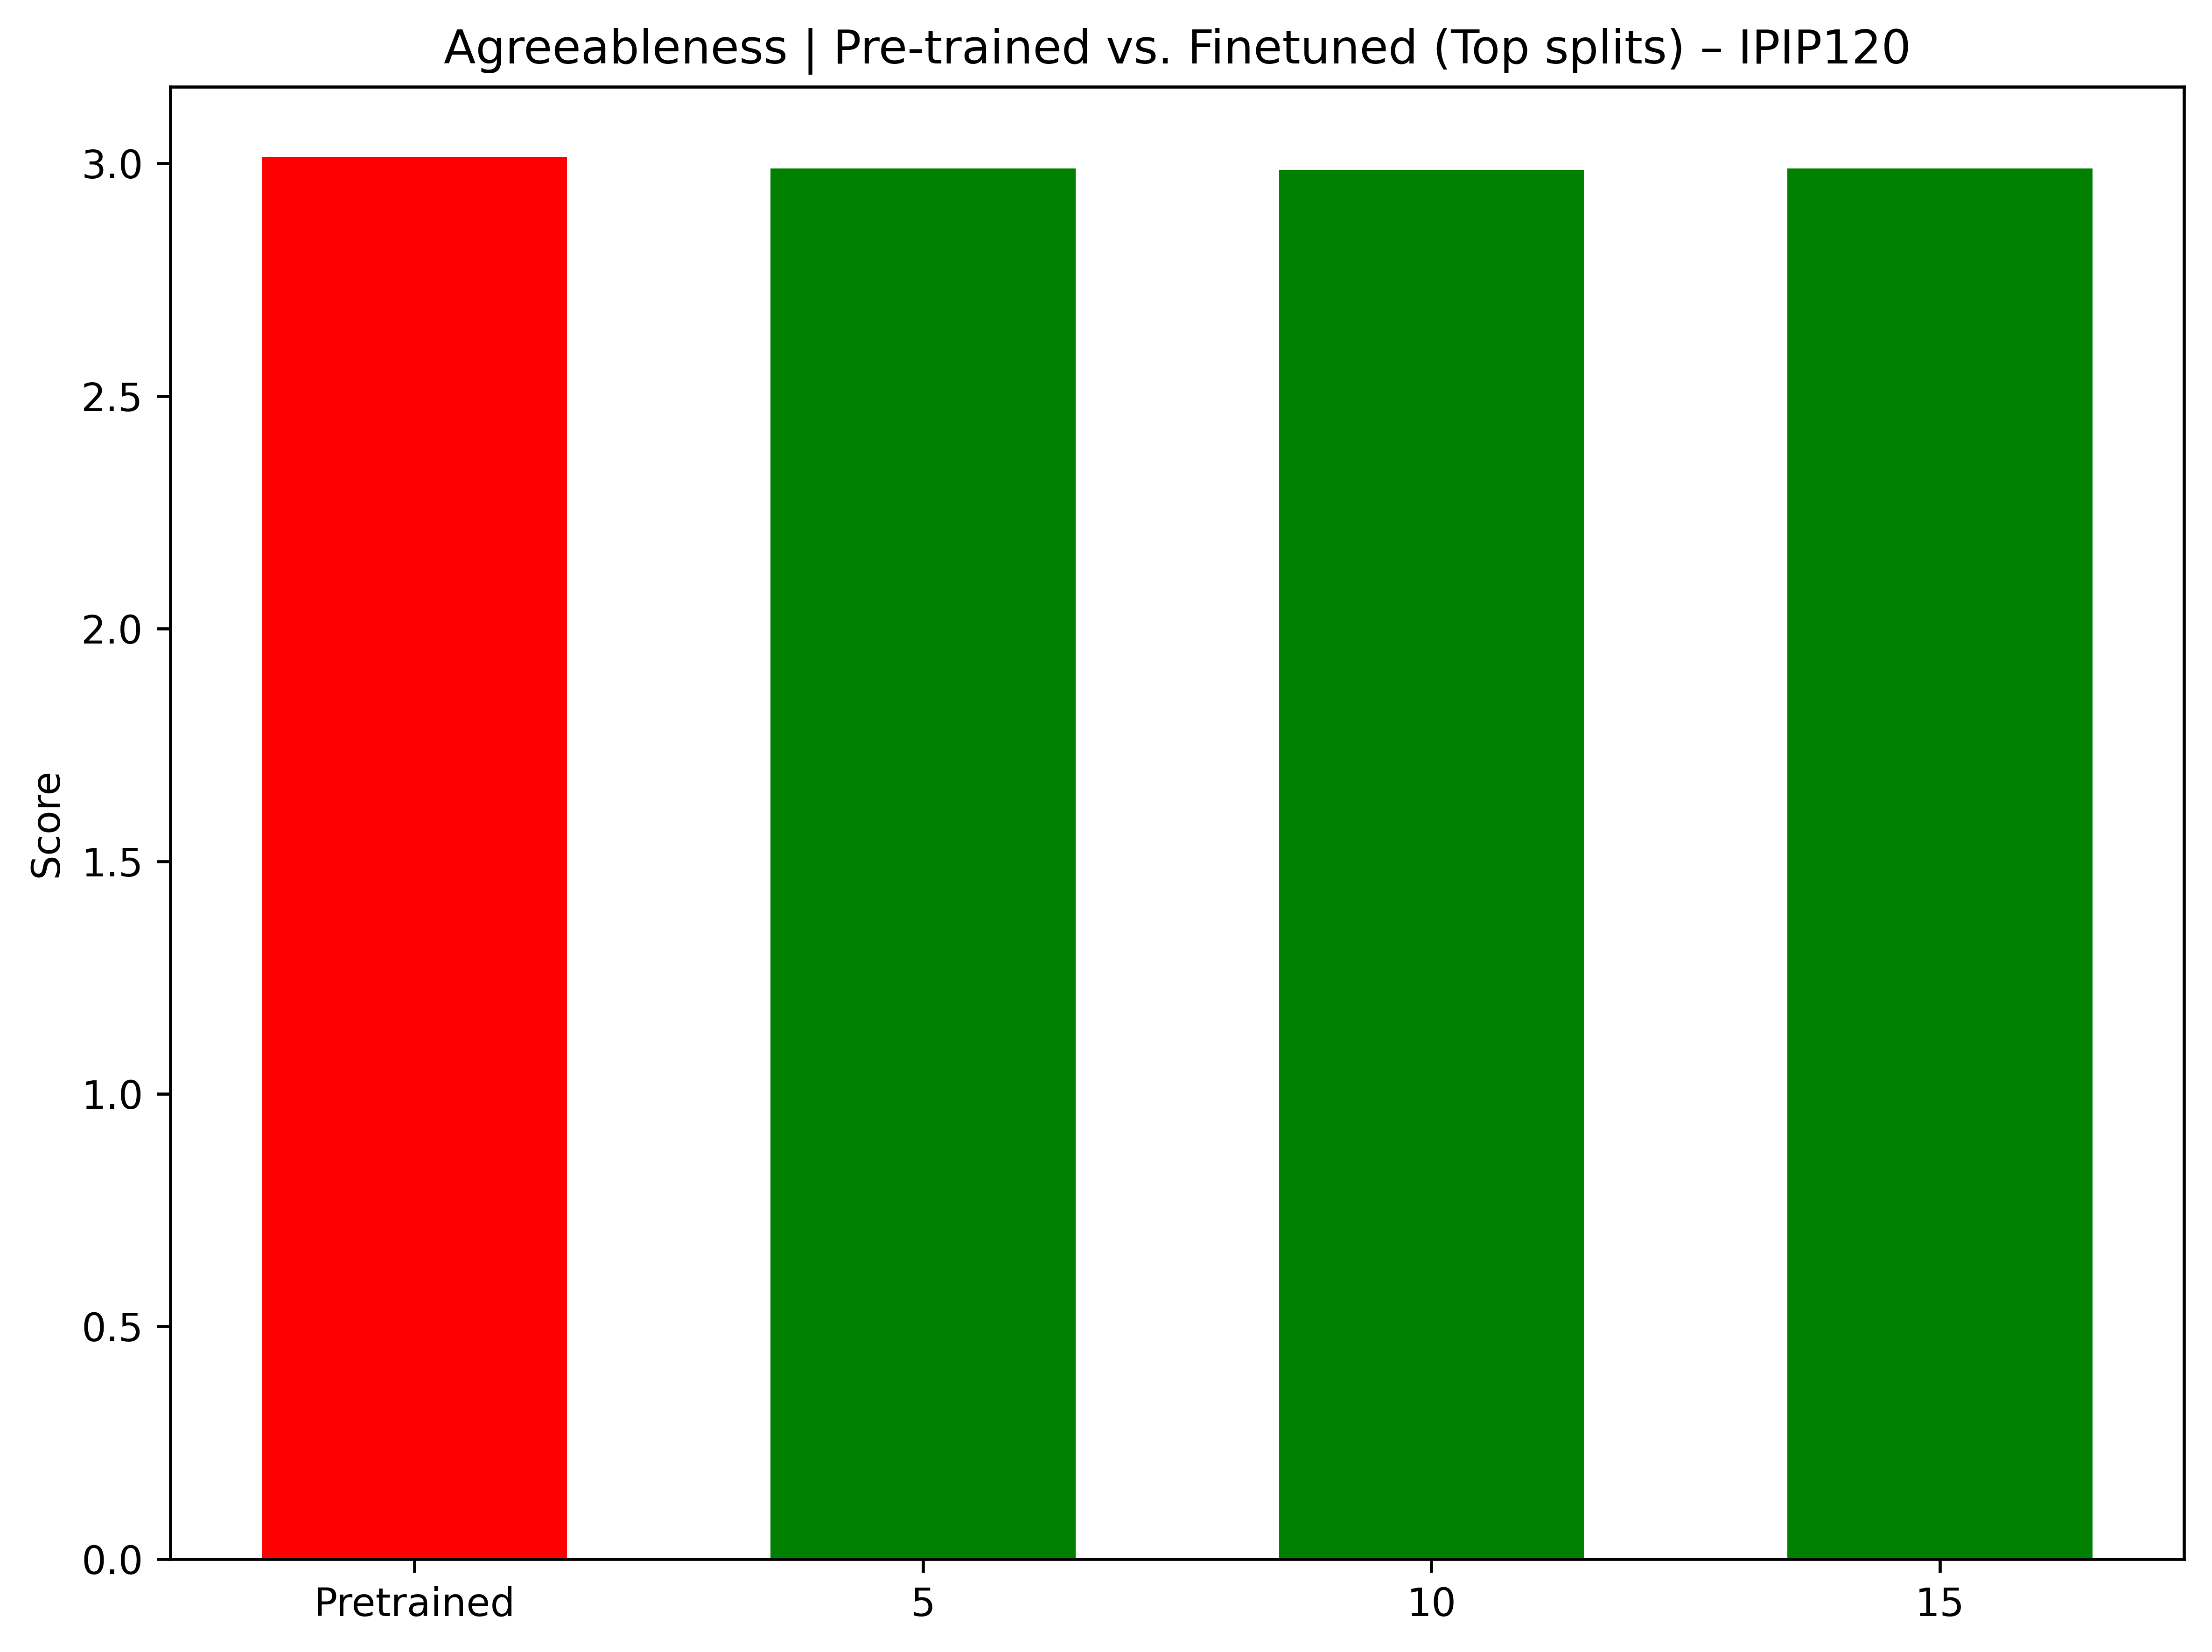
\includegraphics[width=0.8\textwidth]{img/results/w_i_H1_IPIP120_Agreeableness_top.png}
    \caption{Conscientiousness scores | Pre-trained vs. Finetuned on bottom Pandora splits | BFI-10}
    \label{fig:w_i_H1_BFI10_Agreeableness_bottom}
\end{figure}

\begin{figure}[H]
    \centering
    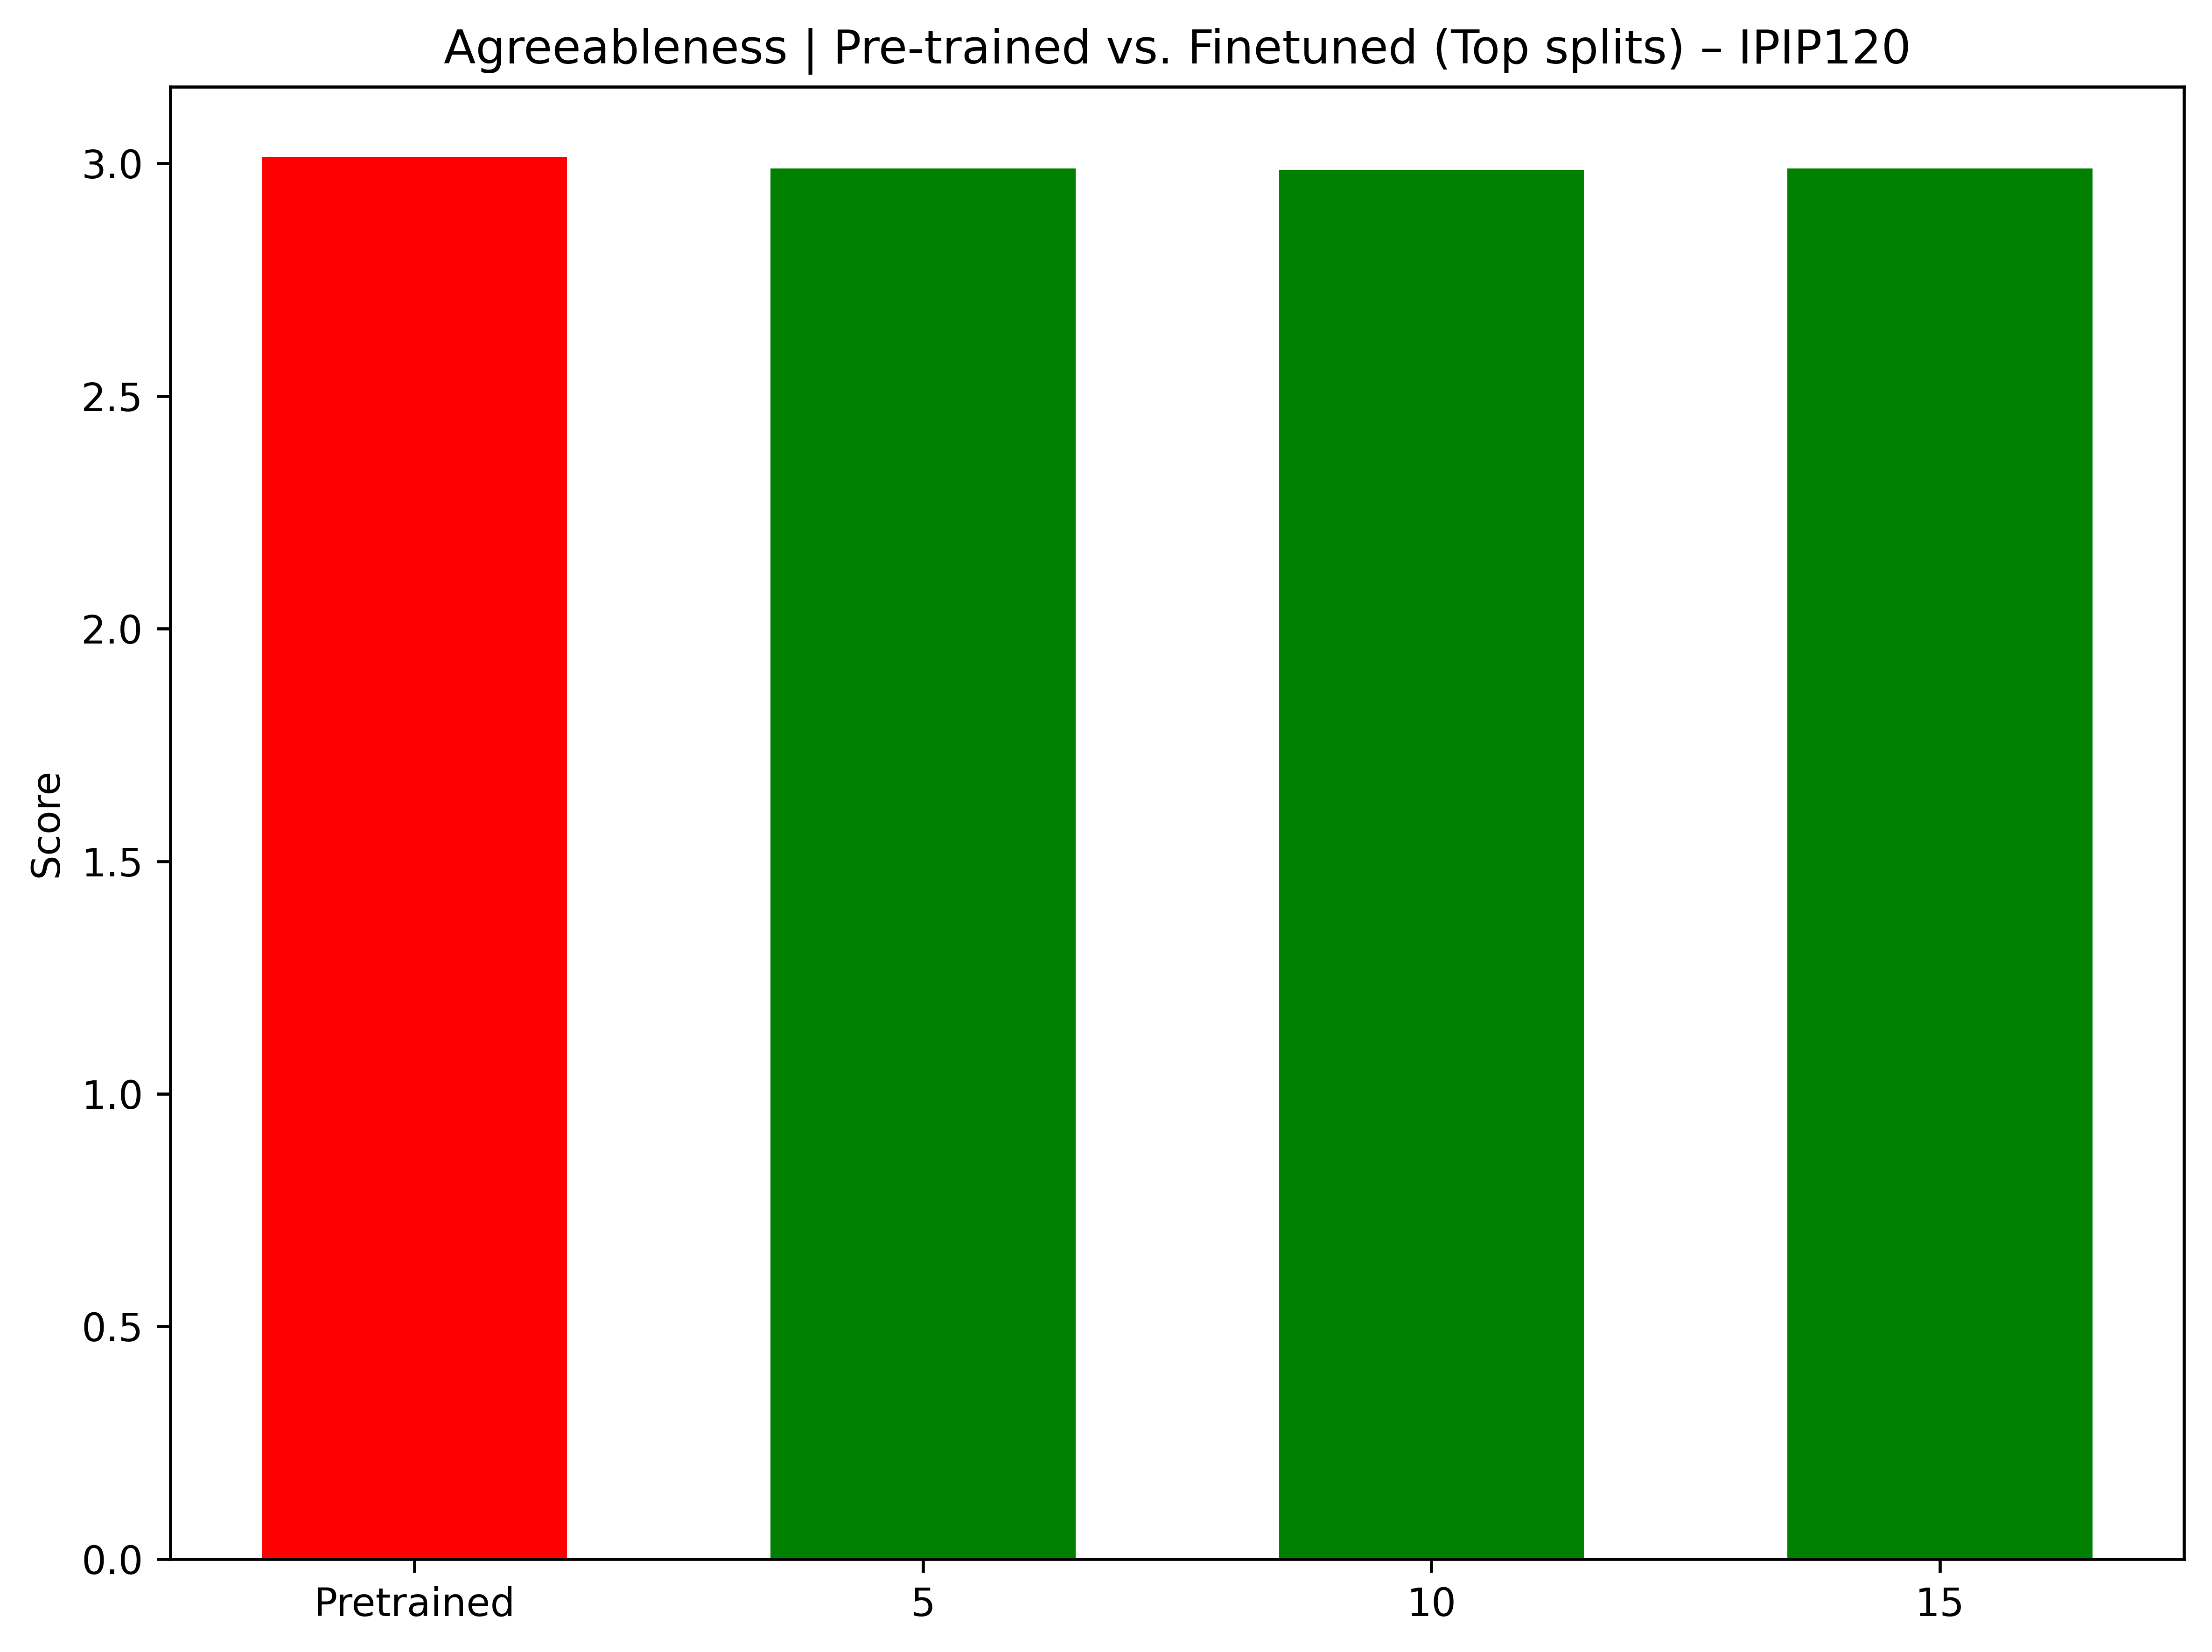
\includegraphics[width=0.8\textwidth]{img/results/w_i_H1_IPIP120_Agreeableness_top.png}
    \caption{Conscientiousness scores | Pre-trained vs. Finetuned on bottom Pandora splits | BFI-10}
    \label{fig:w_i_H1_BFI10_Agreeableness_bottom}
\end{figure}

\section{Additional Results}
\subsubsection{Post-finetuning experiment results across all PANDORA splits}
\begin{table}[]
\centering
\resizebox{\columnwidth}{!}{%
\begin{tabular}{cccccccc}
trait             & location & size & Openness           & Conscientiousness  & Extraversion        & Agreeableness       & Neuroticism        \\
openness          & top      & 5    & 97.89873417721519  & 44.55696202531646  & 50.22784810126582   & 47.721518987341774  & 49.734177215189874 \\
openness          & bot      & 5    & 6.556962025316456  & 40.40506329113924  & 18.367088607594937  & 33.75949367088607   & 50.21518987341772  \\
openness          & top      & 10   & 96.75796178343948  & 45.554140127388536 & 49.59872611464968   & 43.89171974522293   & 48.496815286624205 \\
openness          & bot      & 10   & 10.044585987261147 & 41.4140127388535   & 23.94267515923567   & 35.37579617834395   & 50.99363057324841  \\
openness          & top      & 15   & 95.41949152542372  & 42.12076271186441  & 48.70338983050848   & 44.019067796610166  & 47.19915254237288  \\
openness          & bot      & 15   & 13.474576271186441 & 42.851694915254235 & 24.79237288135593   & 37.91101694915254   & 48.75              \\
conscientiousness & top      & 5    & 60.55696202531646  & 95.54430379746836  & 40.50632911392405   & 36.860759493670884  & 30.518987341772153 \\
conscientiousness & bot      & 5    & 72.10126582278481  & 0.5189873417721519 & 35.45569620253165   & 33.9746835443038    & 61.721518987341774 \\
conscientiousness & top      & 10   & 61.37579617834395  & 92.52866242038216  & 41.394904458598724  & 37.955414012738856  & 32.19108280254777  \\
conscientiousness & bot      & 10   & 69.48407643312102  & 1.5987261146496816 & 36.40764331210191   & 35.24203821656051   & 62.738853503184714 \\
conscientiousness & top      & 15   & 62.440677966101696 & 89.86440677966101  & 43.5021186440678    & 40.88135593220339   & 35.105932203389834 \\
conscientiousness & bot & 15 & 68.20762711864407 & 3.0296610169491527 & 35.067796610169495 & 34.766949152542374 & 64.57627118644068 \\
extraversion      & top      & 5    & 78.18987341772151  & 38.9746835443038   & 96.10126582278481   & 43.31012658227848   & 34.5               \\
extraversion      & bot      & 5    & 55.037974683544306 & 36.35443037974684  & 0.43037974683544306 & 42.607594936708864  & 60.607594936708864 \\
extraversion      & top      & 10   & 73.37579617834395  & 41.98726114649681  & 92.92993630573248   & 39.646496815286625  & 34.7484076433121   \\
extraversion      & bot      & 10   & 53.75796178343949  & 33.859872611464965 & 1.197452229299363   & 41.46496815286624   & 60.05095541401274  \\
extraversion      & top      & 15   & 71.79661016949153  & 41.66525423728814  & 89.35593220338983   & 41.34957627118644   & 35.722457627118644 \\
extraversion      & bot      & 15   & 53.59322033898305  & 33.228813559322035 & 2.207627118644068   & 42.682203389830505  & 62.58474576271186  \\
agreeableness     & top      & 5    & 71.50632911392405  & 43.65822784810127  & 32.87341772151899   & 95.9873417721519    & 47.848101265822784 \\
agreeableness     & bot      & 5    & 64.4746835443038   & 47.462025316455694 & 39.95569620253165   & 0.24050632911392406 & 38.10126582278481  \\
agreeableness     & top      & 10   & 69.22292993630573  & 43.92356687898089  & 35.203821656050955  & 93.14012738853503   & 47.738853503184714 \\
agreeableness     & bot      & 10   & 65.86942675159236  & 43.09235668789809  & 37.04140127388535   & 1.2101910828025477  & 42.52229299363057  \\
agreeableness     & top      & 15   & 68.41525423728814  & 45.67796610169491  & 36.182203389830505  & 90.5635593220339    & 50.41101694915254  \\
agreeableness     & bot      & 15   & 63.00635593220339  & 42.78177966101695  & 38.57415254237288   & 2.6016949152542375  & 42.936440677966104 \\
neuroticism       & top      & 5    & 61.620253164556964 & 20.848101265822784 & 18.70886075949367   & 38.56962025316456   & 98.0126582278481   \\
neuroticism       & bot      & 5    & 69.78481012658227  & 50.88607594936709  & 50.79746835443038   & 35.25316455696203   & 0.9746835443037974 \\
neuroticism       & top      & 10   & 62.29936305732484  & 21.54140127388535  & 20.840764331210192  & 41.681528662420384  & 96.29299363057325  \\
neuroticism       & bot      & 10   & 67.35668789808918  & 50.203821656050955 & 48.560509554140125  & 32.94267515923567   & 2.535031847133758  \\
neuroticism       & top      & 15   & 62.54237288135593  & 23.89830508474576  & 24.377118644067796  & 40.66525423728814   & 94.53389830508475  \\
neuroticism       & bot      & 15   & 63.53813559322034  & 50.63135593220339  & 47.317796610169495  & 36.440677966101696  & 4.067796610169491 
\end{tabular}%
}
\caption{Post-finetuning experiment results across OCEAN labels for PANDORA splits}
\label{tab:post-ft-results}
\end{table}

\end{document}
